
 
\documentclass[sn-mathphys,Numbered]{sn-jnl}% Math and Physical Sciences Reference Style
%\documentclass[sn-mathphys,Numbered,draft]{sn-jnl}% Math and Physical Sciences Reference Style

%%\documentclass[sn-nature]{sn-jnl}% Style for submissions to Nature Portfolio journals
%%\documentclass[sn-basic]{sn-jnl}% Basic Springer Nature Reference Style/Chemistry Reference Style
%%\documentclass[sn-aps]{sn-jnl}% American Physical Society (APS) Reference Style
%%\documentclass[sn-vancouver,Numbered]{sn-jnl}% Vancouver Reference Style
%%\documentclass[sn-apa]{sn-jnl}% APA Reference Style 
%%\documentclass[sn-chicago]{sn-jnl}% Chicago-based Humanities Reference Style
%%\documentclass[default]{sn-jnl}% Default
%%\documentclass[default,iicol]{sn-jnl}% Default with double column layout

%%%% Standard Packages
%%<additional latex packages, if required can be included here>

\setlength{\parskip}{\baselineskip}

\usepackage{graphicx}%
\usepackage{amsmath,amssymb,amsfonts,bm}%
\usepackage{multirow}
\usepackage{amsthm}%
%\usepackage{subcaption}
\usepackage{mathrsfs}%
\usepackage[title]{appendix}%
\usepackage{xcolor}%
\usepackage{textcomp}%
\usepackage{manyfoot}%
\usepackage{booktabs}%
%\usepackage{algorithm}%
%\usepackage{algorithmicx}%
\usepackage{algpseudocode}%
\usepackage{listings}%
\usepackage{bigints}
\usepackage{outlines}
\usepackage{geometry}
\usepackage{subfigure}
\usepackage{siunitx}
\usepackage{float}

\geometry
{
a4paper,         % or letterpaper
textwidth=15cm,  % llncs has 12.2cm
textheight=24cm, % llncs has 19.3cm
% heightrounded,   % integer number of lines
% hratio=1:1,      % horizontally centered
% vratio=2:3,      % not vertically centered
}
\setlength{\tabcolsep}{0.5cm}
\usepackage[onehalfspacing]{setspace}
% \usepackage{lineno}
% \linenumbers
%%%%

\usepackage[utf8]{inputenc}
\usepackage{graphicx}
\usepackage[ruled,vlined]{algorithm2e}
\usepackage{amsmath}
%\usepackage{movie15} %to allow movie embedding
\usepackage[section]{placeins}
\usepackage{enumitem}
\usepackage{color,soul}
\usepackage{xfrac}

%% New math commands
\newcommand{\s}[1]{\overset{*}{#1}}
\newcommand{\RM}{\bm{\Lambda}}
\newcommand{\RMI}{\bm{\Lambda}_0}
\newcommand{\RMT}{\bm{\Lambda}_t}
\newcommand{\RV}{\bm{\psi}}
\newcommand{\magRV}{\psi}
\newcommand{\RMTS}{\s{\bm{\Lambda}}_t}
\newcommand{\bb}{\boldsymbol}

%% For contact
\newcommand{\rbar}{\bar{\bm{r}}}
\newcommand{\xibar}{\bar{\xi}}
%\newcommand{\magRV}{\bbit{\psi}}
\newcommand{\diag}{\rm diag}

\begin{document}

\title[Article Title]{Assessing the potential of Jacobian-free Newton-Krylov methods for cell-centred finite volume solid mechanics}

\author*[1,2,3]{\fnm{Philip} \sur{Cardiff}}\email{philip.cardiff@ucd.ie}
\author[4]{\fnm{Ivan} \sur{Batisti\'{c}}}
\author[4]{\fnm{\v{Z}eljko} \sur{Tukovi\'{c}}}

\affil*[1]{\orgdiv{School of Mechanical and Materials Engineering}, \orgname{University College Dublin}, \orgaddress{\country{Ireland}}}
\affil[2]{\orgdiv{UCD Centre for Mechanics}, \orgname{University College Dublin}, \orgaddress{\country{Ireland}}}
\affil[3]{\orgdiv{SFI I-Form Centre}, \orgname{University College Dublin}, \orgaddress{\country{Ireland}}}
\affil[4]{\orgdiv{Faculty of Mechanical Engineering and Naval Architecture}, \orgname{University of Zagreb}, \orgaddress{\country{Croatia}}}



\abstract
{
In this study, we explore the efficacy of Jacobian-free Newton-Krylov methods within the context of finite-volume solid mechanics.
Traditional Newton-based approaches to solving nonlinear systems typically require explicit formation and storage of the Jacobian matrix, which can be computationally expensive and memory-intensive.
The Jacobian-free Newton-Krylov method circumvents this by employing Krylov subspace iterative solvers, such as GMRES, in conjunction with a Newton iteration scheme that approximates the action of the Jacobian through finite difference evaluations.
A further potential advantage of the Jacobian-free Newton-Krylov method is that it is readily applicable to existing segregated finite volume frameworks, where forming and storing the exact Jacobian would require major code refactoring.
%This approach promises significant computational savings, especially for large-scale, complex simulations prevalent in solid mechanics.
This article research systematically evaluates the performance of Jacobian-free Newton-Krylov methods by benchmarking them against conventional segregated methods on a suite of benchmark cases of varying geometric dimension, geometric nonlinearity, dynamic response, and material behaviour.
Key metrics such as computational cost, memory and robustness are analysed.
Additionally, we investigate the impact of various solution algorithm choices, such as preconditioning strategy, on the efficiency of the Jacobian-free Newton-Krylov method.
Our findings indicate that Jacobian-free Newton-Krylov methods can achieve \hl{comparable/superior/XXX convergence behaviour} relative to traditional segregated methods, particularly in cases where YYYY.
\hl{Summarise key findings: time, memory, important choices, JFNK vs SEG vs FE, ...}
The results suggest that Jacobian-free Newton-Krylov methods are promising for advancing finite-volume solid mechanics simulations and are particularly attractive for existing segregated frameworks where minimal code changes would be required to exploit openly available Jacobian-free Newton-Krylov implementations.
The described implementations are made publicly available in the solids4foam toolbox for OpenFOAM, allowing the community to examine, extend and compare the procedures with the our codes.
%offering a viable pathway for enhancing computational efficiency and scalability.
%EMPHASISE: easy to extend segregated frameworks, on contrast to exact Jacobian methoods.
%This study provides critical insights and practical guidelines for implementing JFNK methods in engineering and scientific applications.
%Key FV points:
%- many FV codes were developed around a segregated solution procedure, which requires significant effort to extend to a full Newton method, e.g. in terms of Jacobian assembly, storage, and linear system solution.
%- this paper examines Jacobian-free Newton-Krylov as a straight-forward extension of the segregated approach, without the need for a full Jacobian based method.
%- compact approximate Jacobian for preconditioner (more compact than FE approach)
%- implemented in OpenFOAM, and code and cases are made publicly available.
}



\keywords{Jacobian-free Newton-Krylov, Finite volume method, GMRES, OpenFOAM}

\maketitle


%%%%%%%%%%%%%%%%%%%%%%%%%%%%%%%%%%%%%%%%%%%%%%%%%%%%%%%%%%%%%%%%%%
\section{Introduction}\label{sec:intro}
%%%%%%%%%%%%%%%%%%%%%%%%%%%%%%%%%%%%%%%%%%%%%%%%%%%%%%%%%%%%%%%%%%
%Paper outline:
%
%Intro
%- FV is of interest for CSM
%- Most methods use segregated algorithms, stemming from CFD algorithms
%- Extension to block-coupled Newton methods is not easy, in terms of derivation, and code refactoring (matrix storage, extended stencil, linear solver, etc.).
%- JFNK promises the performance of Newton methods, but without the need to form the full Jacobian. Define JFNK method. Hence, an existing segregated code can easily be adapted to use JFNK without major refactoring, albeit this process is made easier by the availability of open-source JFNK implementations.
%- this paper examines JFNK for linear and nonlinear FV CSM procedures, where the compact stencil approximate Jacobian is used for preconditioning.
Finite volume formulations for solid mechanics are heavily influenced by their fluid mechanics counterparts, favouring segregated implicit and fully explicit methods.
Segregated approaches, where the governing momentum equation is temporarily decomposed into scalar component equations, offer memory efficiency and simplicity of implementation, but the outer coupling Picard iterations often suffer from slow convergence.
Explicit formulations are straightforward to implement and offer superior robustness but are only efficient for high-speed dynamics, where the physics requires small time increments.
In contrast, the finite element community commonly employs Newton-Raphson-type solution algorithms, which necessitate repeated assembly of the Jacobian matrix and solution of the resulting block-coupled non-diagonally dominant linear system.
A disadvantage of traditional Newton-based approaches is that they typically require explicit formation and storage of the Jacobian matrix, which can be computationally expensive and memory-intensive.
A further disadvantage from a finite volume perspective is that extending existing code frameworks from segregated algorithms to a coupled Newton-Raphson-type approach is challenging in terms of the required assembly, storage, and solution of the resulting block-coupled system.
In addition, the derivation of the true Jacobian matrix is non-trivial.
Consequently, similar block-coupled solution finite volume methods are rare in the literature \citep{Das2011, Cardiff2016, Castrillo2024}.
The motivation of the current work is to seek (or exceed) the robustness and efficiency of block-coupled Newton-Raphons approaches in a way that can be easily incorporated into existing segregated solution frameworks.
To this end, the current article examines the efficacy of \emph{Jacobian-free} Newton-Krylov methods, where the quadratic convergence of Newton methods can potentially be achieved without deriving, assembling and storing the exact Jacobian.

Jacobian-free Newton-Krylov methods circumvent the need for the Jacobian matrix by combining the Newton-Raphson method with Krylov subspace iterative linear solvers, such as GMRES, and noticing that such Krylov solvers do not explicitly require the Jacobian matrix.
Instead, only the action of the Jacobian matrix on a solution-type vector is required.
The key step in Jacobian-free Newton-Krylov methods is the approximation of products between the Jacobian matrix and a vector using the finite difference method; that is
\begin{eqnarray}
	\bb{J} \bb{v} \approx \frac{\bb{F}(\bb{x} + \epsilon \bb{v}) - \bb{F}(\bb{x})}{\epsilon}
\end{eqnarray}
where $\mathbf{J}$ is the Jacobian matrix, $\mathbf{x}$ is the current solution vector (e.g. nodal displacements), $\mathbf{v}$ is a vector (e.g., from a Krylov subspace), and $\epsilon$ is a small scalar perturbation.
%Determining the appropriate value for $\epsilon$ requires balancing the truncation error of the finite difference approximation and round-off (numerical precision) error.
With an appropriate choice of $\epsilon$ (balancing truncation and round-off errors), the characteristic quadratic convergence of Newton methods can be achieved without the Jacobian, hence the modifier \emph{Jacobian-free}.
This approach promises significant memory savings over Jacobian-based methods, especially for large-scale, but also potentially for execution time, with appropriate choice of solution components.

A crucial aspect of ensuring the efficiency and robustness of the Jacobian-free Newton-Krylov method is the choice of a suitable preconditioner for the Krylov iterations.
This preconditioner is often derived from the exact Jacobian matrix in traditional Newton methods.
However, the Jacobian-free approach does not allow direct access to the full Jacobian matrix, necessitating an alternative strategy to approximate its action.
To this end, and to extend existing segregated frameworks, we propose using a compact-stencil approximate Jacobian as the preconditioner. This approximate Jacobian corresponds to the matrix typically employed in segregated approaches; similar approaches are successful in fluid mechanics applications \citep{Nishikawa2020, nonNewtonianJFNKPaper}; however, it is unclear if such an approach is suitable for solid mechanics - a question which we hope to answer in this work.
By leveraging this compact-stencil approximate Jacobian, we aim to effectively precondition the Krylov iterations, enhancing convergence while maintaining the memory and computational savings that define the Jacobian-free and segregated methods.
Similarly, if such an approach is efficient, it would naturally fit into existing segregated frameworks, as existing matrix storage and assembly can be reused.

The remainder of the paper is structured as follows:
Section 2 summarises a typical solid mechanics mathematical model and its cell-centred finite volume discretisation.
Section 3 presents the solution algorithms, starting with the classic segregated solution algorithm, followed by the proposed Jacobian-free Newton-Krylov solution algorithm.
The performance of the proposed Jacobian-free Newton-Krylov approach is compared with the segregated approach on several varying benchmark cases in Section 4, where the effect of several factors are examined, including problem dimension, mesh, material model, nonlinear geometry, choice of preconditioner, and other solution parameter.
Finally, the article ends with a summary of the main conclusions of the work.


%%%%%%%%%%%%%%%%%%%%%%%%%%%%%%%%%%%%%%%%%%%%%%%%%%%%%%%%%%%%%%%%%%
\section{Mathematical Model and Numerical Methods}\label{sec:math_model}
%%%%%%%%%%%%%%%%%%%%%%%%%%%%%%%%%%%%%%%%%%%%%%%%%%%%%%%%%%%%%%%%%%

%
%Math model and numerical methods
%- General governing equation -> unknown D; limit ourselves to compressibility

\subsection{Governing Equations} \label{sec:governing_eqn}

In this work, we restrict our interest to Lagrangian formulations of the conservation of linear momentum.
Assuming small strains, the linear geometry formulation is expressed in strong integral form as:
\begin{eqnarray} \label{eqn:momentum_lingeom}
    \int_{\Omega} \rho \frac{\partial^2 \bb{u} }{\partial t^2} \, d\Omega
    =
    \oint_{\Gamma} \bb{n} \cdot \bb{\sigma}_s \,  d\Gamma
    + \int_{\Omega}  \bb{f}_b \, d\Omega
\end{eqnarray}
where $\Omega$ is the volume of an arbitrary body bounded by a surface $\Gamma$ with outwards pointing normal $\bb{n}$.
The density is $\rho$, $\bb{u}$ is the displacement vector, $\bb{\sigma}_s$ is the engineering (small strain) stress tensor, and $\bb{f}_b$ is a body force per unit volume, e.g., $\rho \bb{g}$, where $\bb{g}$ is gravity.

More generally,  linear momentum conservation can be expressed in a nonlinear geometry form, which is suitable for finite strains.
Two equivalent nonlinear geometry forms are common: the \emph{total} Lagrangian form:
\begin{eqnarray} \label{eqn:momentum_TL}
    \int_{\Omega_o} \rho_o \frac{\partial^2 \bb{u} }{\partial t^2} d\Omega_o
    =
    \oint_{\Gamma_o} \left( J \bb{F}^{-T} \cdot \bb{n}_o \right) \cdot \bb{\sigma} \ d\Gamma_o
    + \int_{\Omega_o}  \bb{f}_b \, d\Omega_o
\end{eqnarray}
and the \emph{updated} Lagrangian form:
\begin{eqnarray} \label{eqn:momentum_UL}
    \int_{\Omega_u} \frac{\partial }{\partial t} \left( \rho_u \frac{\partial \bb{u} }{\partial t} \right) d\Omega_u
    = \oint_{\Gamma_u}(j\bb{f}^{-T}\cdot{\bb{n}_u)\cdot \bb{\sigma}}\ d\Gamma_u
    + \int_{\Omega_u}  \bb{f}_b \, d\Omega_u
\end{eqnarray}
where subscript $o$ indicates quantities in the initial reference configuration, and subscript $u$ indicates quantities in the updated configuration.
The true (Cauchy) stress tensor is indicated by $\bb{\sigma}$.

The deformation gradient is defined as $\bb{F} = \textbf{I} + (\bb{\nabla} \bb{u})^T$ and its determinant as $J = \text{det}(\bb{F})$.
Similarly, the \emph{relative} deformation gradient is given in terms of the displacement \emph{increment} as $\bb{f}=\textbf{I} + \left[\bb{\nabla}(\Delta \bb{u}) \right]^T$ and its determinant as $j = \text{det}(\bb{f})$.
The displacement increment is the change in displacement between the current time step and the previous time step when the time interval is discretised into a finite number of steps.

%The two forms are connected through Nanson’s formula \cite{bathe_finite_1996}, which relate the deformed area vector $\bb{\Gamma}$ with the initial area vector $\bb{\Gamma}_{o}$:
%\begin{equation}
%    \bb{\Gamma} = J\bb{F}^{-T}\cdot\bb{\Gamma}_o
%\end{equation}


%Although the total Lagrangian approach is a viable option for wire drawing, the current work adopts the updated Lagrangian approach as developing Eulerian-type upstream and downstream conditions (Section \ref{sec:euler_BCs}) is conceptually easier in an updated Lagrangian formulation.

The definition of the engineering stress ($\bb{\sigma}_s$) and true stress ($\bb{\sigma}$) in Equations \ref{eqn:momentum_lingeom}, \ref{eqn:momentum_TL} and \ref{eqn:momentum_UL} is given by a chosen mechanical law, e.g. linear elasticity.
Several mechanical laws are considered in this work, as briefly described in Section \ref{sec:test_cases}.



%%--------------------------------------------------------------------------------------------------------------------%%
\subsection{Newton-Type Solution Methods}
%%--------------------------------------------------------------------------------------------------------------------%%
To facilitate the comparison between classic segregated solution algorithms and the proposed Jacobian-free Newton-Krylov algorithm, the governing linear momentum conservation (Equations \ref{eqn:momentum_lingeom}, \ref{eqn:momentum_TL} and \ref{eqn:momentum_UL}) is expressed in the general form:
\begin{eqnarray} \label{eqn:residual}
	\mathcal{R}(\bb{u}) = \bb{0}
\end{eqnarray}
where $\mathcal{R}$ represents the \emph{residual} (imbalance) of the equation, which is a function of the primary unknown field.
For example, in the linear geometry case, the residual is given as
\begin{eqnarray}
    \bb{R}(\bb{u})
    \;=\;
    \oint_{\Gamma} \bb{n} \cdot \bb{\sigma}_s(\bb{u}) \,  d\Gamma
    + \int_{\Omega}  \rho \bb{g} \, d\Omega
    -  \int_{\Omega} \rho \frac{\partial^2 \bb{u} }{\partial t^2} \, d\Omega
    \;=\; \bb{0}
\end{eqnarray}
where the dependence of the stress tensor on the solution vector is made explicitly clear: $\bb{\sigma}_s(\bb{u})$.



In Newton-type methods, a Taylor expansion about a current point $\bb{u}_k$ can be used to solve Equation \ref{eqn:residual} \cite{Knoll2004}:
\begin{eqnarray}
	\bb{R}(\bb{u}_{k+1}) = \bb{R}(\bb{u}_{k}) \;+\;  \bb{R}'(\bb{u}_{k}) (\bb{u}_{k+1} - \bb{u}_{k}) \;+\; \text{H.O.T.} = \bb{0}
\end{eqnarray}
Neglecting the higher-order terms ($\text{H.O.T.}$) yields the strict Newton method in terms of an iteration over a sequence of linear systems: 
\begin{eqnarray} \label{eq:NewtonRaphson}
	\bb{J}(\bb{u}_k) \delta \bb{u} &=& -\bb{R}(\bb{u}_n), \notag \\
	\bb{u}_{k+1} &=& \bb{u}_k + s \, \delta \bb{u}, \notag \\
	\quad
	k &=& 0,1,...
%    \label{eq:NewtonRaphsonA}
%    \overbrace{\left[ \frac{\partial \mathcal{R}(\bb{u})}{\partial \bb{u}} \right]_n}^{\mathcal{J}} \Delta \bb{u} = -\mathcal{R}(\bb{u})_n \\
%    \label{eq:NewtonRaphsonB}
%    \bb{u}_{n+1} = \bb{u}_{n} + \alpha \Delta \bb{u}
\end{eqnarray}
where $\bb{J} \equiv \bb{R}'$ is the Jacobian matrix.
Starting the Newton procedure requires the specification of $\bb{u}_0$.
%is iteratively solved by linearisation about the current value of the solution, leading to a linear system and iterative update of the solution vector:
%\begin{eqnarray}
%    \label{eq:NewtonRaphsonA}
%    \overbrace{\left[ \frac{\partial \mathcal{R}(\bb{u})}{\partial \bb{u}} \right]_n}^{\mathcal{J}} \Delta \bb{u} = -\mathcal{R}(\bb{u})_n \\
%    \label{eq:NewtonRaphsonB}
%    \bb{u}_{n+1} = \bb{u}_{n} + \alpha \Delta \bb{u}
%\end{eqnarray}
%where subscript $n$ indicates the outer (Newton) iteration index.
The scalar $s > 0$ can be chosen to improve convergence, for example, using a line search or under-relaxation procedure, and is equal to unity in the classic Newton-Raphson approach.
Iterations are performed over this system until the residual $\bb{R}(\bb{u}_n)$ and solution correction $\delta \bb{u}$ are sufficiently small, with appropriate normalisation.

%\hl{$\Delta u$: we are using in two ways: increment and correction. Fix this!}
%\hl{KnollKeyes give a nice concise description of Newton: check}

For problems with $N$ scalar equations and $N$ scalar unknowns, the residual $\bb{R}$ and solution $\bb{u}$ vectors have dimensions of $N \times 1$. %, while the Jacobian matrix has dimensions of $N \times N$.
%In contrast, for vector problems, like the solid mechanics problems considered in this work, the residual and solution vectors have dimensions of $N_d N \times 1$ and the Jacobian matrix has dimensions of $N_d N \times N_d N$, where $N_d$ is the geometric dimension of the problem, e.g. $N_d = 2$ for 2-D and $N_d = 3$ for 3-D.
The components of the $N \times N$ Jacobian are
\begin{eqnarray} \label{eq:J}
	{J}_{ij} = \frac{\partial {R}_i (\bb{u})}{\partial u_j}
\end{eqnarray}

In the current work, we are interested in vector problems, where the governing momentum equation is formulated in terms of the unknown displacement solution vector.
In this case, Equation \ref{eq:J} refers to the individual scalar components of the residual, solution, and Jacobian.
That is, for 3-D analyses, the residual takes the form
\begin{eqnarray}
	\bb{R}(\bb{u}) = \left\{ R_1^x, R_1^y, R_1^z, R_2^x, R_2^y, R_2^z, ..., R_n^z \right\}
\end{eqnarray}
and the solution takes the form
\begin{eqnarray}
	\bb{u} = \left\{ u_1^x, u_1^y, u_1^z, u_2^x, u_2^y, u_2^z, ..., u_n^z \right\}
\end{eqnarray}
In practice, it is often more practical and efficient to form and store the residual, solution and Jacobian in a \emph{blocked} manner, where the residual and solution can be considered as vectors of vectors.
Similarly, the Jacobian can be formed in terms of sub-matrix block coefficients.

In the strict Newton procedure, the residuals converge at a quadratic rate when the current solution is close to the true solution; that is, the iteration error decreases proportionally to the square of the error at the previous iteration.
Once the method gets sufficiently close to the true solution, the number of correct digits in the approximation roughly doubles with each iteration. 
However, quadratic convergence is only possible when using the exact Jacobian.
In contrast, a quasi-Newton method uses an approximation to the Jacobian, sacrificing strict quadratic convergence in an attempt to produce an overall more computationally efficient procedure.
From this perspective, the segregated solution algorithm commonly employed in finite volume solid mechanics can be viewed as a quasi-Newton method, where an approximate Jacobian replaces the exact Jacobian: 
\begin{eqnarray} \label{eq:Seg}
    \bb{\tilde{J}}(\bb{u}_k) \;\delta \bb{u} = -\bb{R}(\bb{u}_k)
\end{eqnarray}
In this case, the approximate Jacobian $\bb{\tilde{J}}$ comes from the compact stencil discretisation of a simple diffusion (Laplacian) term.
A benefit of this approach is that the inter-component coupling is removed from the Jacobian, allowing the solution of three smaller scalar systems rather than one larger vector system in 3-D (or two smaller systems in 2-D).

A fully explicit procedure can also be viewed from this perspective by selecting an approximate Jacobian which is diagonal $\bb{\tilde{D}}$, making solution of the linear system trivial:
\begin{eqnarray} \label{eq:exp}
    \bb{\tilde{D}}(\bb{u}_k) \;\delta \bb{u} = -\bb{R}(\bb{u}_k)
\end{eqnarray}


%%--------------------------------------------------------------------------------------------------------------------%%
\subsection{Cell-Centred Finite Volume Discretisation}
\label{sec:discretisation}
%%--------------------------------------------------------------------------------------------------------------------%%
In this work, a nominally second-order cell-centred finite volume discretisation is employed, as described previously, for example, \citep{Cardiff2017, batistic2022, tukovic2013, jasak2000}.
Consequently, only a summary of the discretisation is presented below.

The solution domain is discretised in both space and time.
The total simulation period is divided into a finite number of time increments, denoted as $\Delta t$, and the discretised governing momentum equation is solved iteratively in a time-marching fashion. The spatial domain is partitioned into a finite number of contiguous convex polyhedral cells.
%The proposed solution discretisation follows closely the approach of \citet{cardiff_lagrangian_2017}; consequently, only an overview of the final discretised form of equations and adopted solution algorithm are given below.

The conservation equation (Equations \ref{eqn:momentum_lingeom}, \ref{eqn:momentum_TL}, or \ref{eqn:momentum_UL}) is applied to each cell (control volume) in the computational mesh and discretised in terms of the displacement at the cell centre/centroid $\bb{u}_P$ and at the centres of the neighbouring cells $N_i$.

To complete the discretisation, the volume integrals and surface integrals in the governing equation must be approximated by algebraic equations.
Starting first with the volume integrals, assuming a linear variation of the integrand, the mid-point rule approximates the integral in terms of the cell centre value.
Consequently, the inertia term (e.g. left-hand side term of Equation \ref{eqn:momentum_lingeom}) becomes
\begin{eqnarray} \label{eq:inertia}
	\int_{\mathrm{\Omega}} \rho \frac{\partial \bb{u} }{\partial t}  d\mathrm{\Omega}
	\;&\approx&\;
	\rho_P \left(\frac{\partial^2 \bb{u} }{\partial t^2}\right)_P  \Omega_P
\end{eqnarray}
and, similarly, the body force term (e.g. the second term on the right-hand side of Equation \ref{eqn:momentum_lingeom}) becomes:
\begin{eqnarray}
	\int_{\mathrm{\Omega}} \, \rho \, \bb{g} \,  d\mathrm{\Omega}
	\;&\approx&\;
	\rho_P \, \bb{g}\,  \Omega_P
\end{eqnarray}
where subscript $P$ indicates a quantity at the cell centre.
The discretisation of the acceleration in time in Equation \ref{eq:inertia} can be achieved using the finite difference method, e.g. first-order Euler, second-order backwards, second-order Newmark-beta.
\hl{Maybe we should give the temporal discretisation for completeness: i.e. 2nd order backwards}

The surface integral term (e.g. first term on the right-hand side of Equation \ref{eqn:momentum_lingeom}), corresponding to the divergence of stress, is discretised by assuming that the stress varies linearly across the face, allowing the mid-point rule to be used:
\begin{equation}
	\oint_{\Gamma} \bb{n} \cdot \bb{\sigma}  \; d\Gamma
	\approx 
	\sum_{f \in N_f} \bb{\Gamma}_{f} \cdot \bb{\sigma}_f
\end{equation}
where subscript $f$ indicates a quantity at the centre of a cell face, and $N_f$ represents the set of neighbouring cells which share a face with cell $P$.
The stress at a face, $\bb{\sigma}_f$, is calculated by linearly interpolating from the adjacent cell centres.
Stress is calculated at the cell centres as a function of the displacement gradient, $\left(\bb{\nabla}\bb{u}\right)_f$, and the cell-centre gradients are determined using a least squares method \cite{noauthor_openfoam_2015}.

The discretisation is complete but, in its current form, is known to suffer from zero-energy modes, i.e. checkerboarding oscillations.
Here, a Rhie-Chow-type stabilisation term \cite{Rhie1983} is added to the residual (Equation \ref{eqn:residual}) to quell such oscillations.
The Rhie-Chow stabilisation term, first used for finite volume solid mechanics by  \citet{Demirdzic1995}, consists of the numerical difference between a diffusion (Laplacian) term calculated using compact and larger computational stencils.
The term introduces numerical diffusion to the discretisation, which reduces at a third-order rate.
% based on the earlier approach of Rhie and Chow \citet{demirdzic_numerical_1995}.
%One issue encountered with the finite volume method is that the discretisation of the governing conservation of momentum equation ( can be unstable and is known to suffer from checker-boarding errors .
%In order to rectify these issues, the Rhie-Chow stabilisation term \cite{rhie_numerical_1983} as introduced into solid mechanics by  is added to the discretised divergence of the stress in equation \ref{eqn:MomentumImplicitExplicit}.
In the current approach, the Rhie-Chow stabilisation term $\mathcal{D}_{\text {Rhie-Chow }}$ for a cell $P$ takes the following form:
\begin{equation} \label{eq:RhieChow}
	\mathcal{D}_{\text {Rhie-Chow}}
	= \sum_{f \in N_f} \alpha \bar{K}_f
	\left[
	\left|\bb{\Delta}_f\right| \frac{ \bb{u}_{N_f} - \bb{u}_P}{\left|\bb{d}_f\right|}
	- \bb{\Delta}_f \cdot \left(\bb{\nabla} \bb{u} \right)_f
	\right]
	\left|\bb{\Gamma}_{f}\right| 
\end{equation}
%which comes from the difference between Equations \ref{eq:diffusion} and \ref{eq:diffusion_exp}.
where $\alpha > 0$ is a user-defined parameter for globally scaling the amount of stabilisation.
Parameter $\bar{K}_f$ is a stiffness-type parameter that gives the stabilisation an appropriate scale and dimension.
Here, $\bar{K}_f = \frac{4}{3}\mu + \kappa = 2\mu + \lambda$ following previous work \cite{Jasak2008, Cardiff, etc}, where $\mu$ is the shear modulus (first Lam\'{e} parameter), $\kappa$ is the bulk modulus, and $\lambda$ is the second Lam\'{e} parameter.
%where $N_f$ represents the set of faces $f$ in cell $P$, and neighbouring cell centre $N_f$ shares face $f$ with the cell $P$.
Vector $\bb{d}_{f}$ connects cell centre $P$ with the other cell sharing face $f$, and $\bb{n}_{f}$ is the outward-facing unit normal to the face $f$.
The vector $\bb{\Delta}_{f} = \frac{\bb{d}_{f}}{\bb{d}_{f} \cdot \bb{n}_{f}}$ is termed the \emph{over-relaxed orthogonal} vector \cite{Jasak1996} and increases in magnitude as the deviation between the $\bb{d}_{f}$ and $\bb{n}_{f}$ vectors increases.
In this way, the amount of stabilisation increases on distorted meshes.
\hl{Should we mention Nishikawa alpha scheme?} \hl{Very similar: but scales differently with mesh distortion}
%and non-orthogonal correction vector $\bb{k}_f=\bb{n}_f-\bb{\Delta}_f$, where $\bb{n}_f$ is the outward-facing unit normal to the face $f$.
%Vector $\bb{d}_f$ connects the centre of cell $P$ with the centre of cell $N_f$ in the updated configuration.
%The first term on the right-hand side is treated implicitly, while the second term - representing non-orthogonal corrections at the face - is treated in a deferred correction manner.

In Equation \ref{eq:RhieChow}, the first term within the brackets on the right-hand side represents a compact stencil (two-node) approximation of the face normal gradient, while the second term represents a larger stencil approximation.
These two terms cancel out in the limit of mesh refinement (or if the solution varies linearly); otherwise, they produce a stabilisation effect that tends to smooth the solution fields.
As the term reduces at a third-order rate, it does not affect the overall scheme's second-order accuracy.

All dependent variables must be specified at the initial time.
Boundary conditions must be applied to the faces that coincide with the boundary of the solution domain.
The discretised expressions on boundary faces are modified to account for either the known displacement components in Dirichlet conditions or the known traction for Neumann conditions.



\hl{Comment on traction boundaries} \hl{extrapolate to get value or use constitutive law}



%%%%%%%%%%%%%%%%%%%%%%%%%%%%%%%%%%%%%%%%%%%%%%%%%%%%%%%%%%%%%%%%%%
\section{Solution Algorithms}\label{sec:sol_alg}
%%%%%%%%%%%%%%%%%%%%%%%%%%%%%%%%%%%%%%%%%%%%%%%%%%%%%%%%%%%%%%%%%%

%- Seg approach summary
%- JFNK approach summary
%	- implementation via PETSc. Newton with line search, GMRes with MG preconditioner.

%%--------------------------------------------------------------------------------------------------------------------%%
\subsection{Segregated Solution Algorithm} 
\label{sec:seg_alg}
%%--------------------------------------------------------------------------------------------------------------------%%
The classic segregated solution algorithm can be viewed as a quasi-Newton method, where a compact-stencil approximation of a diffusion term is employed as the approximate Jacobian:
%The surface forces Laplacian term (first term on the right-hand side of Equation \ref{eqn:MomentumImplicitExplicit}) is discretised using central differencing with over-relaxed non-orthogonal correction \cite{demirdzic_finite_1993, jasak_application_2000, cardiff_development_2014, cardiff_large_2014, cardiff_lagrangian_2017}:
\begin{eqnarray} \label{eq:diffusion}
	\tilde{\bb{J}} &=& \oint_{\Gamma} \bar{K} \, \bb{n} \cdot \bb{\nabla} \bb{u} \; d\Gamma \notag \\
	&\approx&
	\sum_{f \in N_f} \bar{K}_f \left|\bb{\Delta}_f\right| \left(\frac{\bb{u}_{N_f} - \bb{u}_P}{\left|\bb{d}_f\right|}\right)\left|\bb{\Gamma}_f\right|
%	    &&+ \sum_{f \in N_f} \bar{K}_f \; \bb{k}_f \cdot  \left( \bb{\nabla} \bb{u}\right)_f    \left|\bb{\Gamma}_f\right|
\end{eqnarray}
%where $N_f$ represents the set of faces $f$ in cell $P$, and neighbouring cell centre $N_f$ shares face $f$ with the cell $P$.
%The over-relaxed orthogonal vector $\bb{\Delta}_f = \frac{\bb{d}_f}{\bb{d}_f \cdot \bb{n}_f}$ 
%The non-orthogonal correction vector $\bb{k}_f=\bb{n}_f-\bb{\Delta}_f$.
% where $\bb{n}_f$ is the outward-facing unit normal to the face $f$.
%Vector $\bb{d}_f$ connects the centre of cell $P$ with the centre of cell $N_f$ in the updated configuration.
%The first term on the right-hand side is treated implicitly, while the second term - representing non-orthogonal corrections at the face - is treated in a deferred correction manner.
When a diffusion term is typically discretised using the cell-centre finite volume method, non-orthogonal corrections are included in a deferred correction manner to preserve the order of accuracy on distorted grids.
However, in the Newton method case, the approximate Jacobian's exact value does not affect the final converged solution, but only the convergence behaviour.
Consequently, non-orthogonal corrections are not included in the approximate Jacobian here. However, grid distortion is appropriately accounted for in the calculation of the residual.
Nonetheless, as a result, it is expected that the convergence behaviour of the segregated approach may degrade as mesh non-orthogonality increases.
% since their implicit inclusion would require a coupled solution approach

The linearised system (Equation \ref{eq:Seg}) is formed for each cell in the domain, resulting in a system of algebraic equations:
\begin{eqnarray} \label{eq:SegSys}
    \bb{\tilde{J}}(\bb{u}_n) \; \delta \bb{u} = - \bb{R}(\bb{u}_n)
\end{eqnarray}
where $\bb{\tilde{J}}$ is a symmetric, weakly diagonally dominant, $M \times M$ stiffness matrix, where $M$ is three times the number of cells in 3-D and twice the number of cells in 2-D.
By design, matrix $\bb{\tilde{J}}$  contains no inter-component coupling; consequently, three equivalent smaller linear systems can be formed and solved for the Cartesian components of the displacement correction (or two in 2-D), e.g.
\begin{eqnarray} \label{eq:SegSysX}
     \bb{\tilde{J}}_x(\bb{u}_n)  \;  \Delta \bb{u}_x = - \mathcal{R}_x(\bb{u}_n) \label{eq:segX} \\
     \bb{\tilde{J}}_y(\bb{u}_n)  \;  \Delta \bb{u}_y = - \mathcal{R}_y(\bb{u}_n) \label{eq:segY} \\
     \bb{\tilde{J}}_z(\bb{u}_n)  \;  \Delta \bb{u}_z = - \mathcal{R}_z(\bb{u}_n) \label{eq:segZ}
\end{eqnarray}
where $ \bullet_x$ represents the components in the $x$ direction, $ \bullet_y$ represents the components in the $y$ direction, and $ \bullet_z$ represents the components in the $z$ direction.
An additional benefit of the segregated approach, from a memory perspective, is that matrices $ \bb{\tilde{J}}_x$, $ \bb{\tilde{J}}_y$ and $\bb{\tilde{J}}_z$ are identical, except for the effects from including boundary conditions.
From an implementation perspective, this allows a single scalar matrix to be formed and stored, where the boundary condition contributions are inserted before solving a particular component.

The \emph{inner} linear sparse systems (Equations \ref{eq:segX}, \ref{eq:segY} and \ref{eq:segZ}) can be solved using any typical direct or iterative linear solver approach; however, an incomplete Cholesky pre-conditioned conjugate gradient method \cite{Jacobs1986} is often preferred as the weakly diagonally dominant characteristic leads to good convergence characteristics.
Algebraic multigrid can be used to accelerate convergence.
%In non-linear problems, this system of equations is solved multiple times with updated coefficients in a fixed-point iteration scheme. 
%As noted in previous articles on segregated methods, the inner system need not be solved to a tight tolerance as coefficients and source terms are approximated from the previous increment; a reduction in the residuals of one order of magnitude is typically sufficient. The outer iterations are performed until the predefined tolerance, typically $1 \times 10^{-6}$, has been achieved \cite{cardiff_lagrangian_2017}. 
%In the current updated Lagrangian approach, the mesh is moved to the deformed configuration at the end of each time step rather than after each outer iteration.
%Since the displacements are calculated at the cell centres, a linear least-squared method is employed here \cite{cardiff_lagrangian_2017} to interpolate the displacement increments to the mesh vertices, allowing the mesh to be moved.
%In this method, a linear least squares plane is fit through a vertex and its immediately adjacent cell centres. For boundary vertices, boundary face-centre values are also included in the fitting.
%
%The procedures have been implemented and publicly shared within the solids4foam toolbox \citep{Cardiff2018, Tukovic2018} of the open-source OpenFOAM software.

In literature, the segregated solution algorithm is typically formulated in terms of the total displacement vector (or its difference between time steps) as the primary unknown; in contrast, in the quasi-Newton interpretation presented here, the primary unknown is the correction to the displacement vector, which goes to zero at convergence.
Nonetheless, both approaches are equivalent and neither formulation displays superior performance.

The current procedure is implemented and publicly shared in the solids4foam toolbox of OpenFOAM.
\hl{Add a section about code sharing: appendix?}

\hl{Comment: we have two implementations of segregated: native OpenFOAM (solves Eqs 16-18) and PETSc SNES (solves Eq 15)}
\hl{Do we need to comment on this? Maybe we should use only PETSc SNES for a fair comparison}
\hl{Or we could use both on the verification case and then stick with just one afterwards}



%%--------------------------------------------------------------------------------------------------------------------%%
\subsection{Jacobian-free Newton-Krylov Algorithm}
\label{sec:JFNK_alg}
%%--------------------------------------------------------------------------------------------------------------------%%

%\hl{cite KnollKeyes2004}

As noted in the introduction, the Jacobian-free Newton-Krylov avoids the need to construct the Jacobian matrix explicitly by approximating its action on a solution vector using the finite difference method, repeated here:
\begin{eqnarray} \label{eq:JF}
	\bb{J} \bb{v} \approx \frac{\bb{F}(\bb{x} + \epsilon \bb{v}) - \bb{F}(\bb{x})}{\epsilon}
\end{eqnarray}

%\hl{1}
%Derive Jv for 2x2 system.
The derivation of this approximation can be shown for a $2 \times 2$ system as \cite{Knoll2004}:
\begin{eqnarray}
	\frac{\mathbf{F}(\mathbf{x} + \epsilon \mathbf{v}) - \mathbf{F}(\mathbf{x})}{\epsilon}
	&=&
	\begin{pmatrix}
	\frac{F_1 (x_1 + \epsilon v_1, x_2 + \epsilon v_2) - F_1 (x_1, x_2)}{\epsilon}\\
	\frac{F_2 (x_1 + \epsilon v_1, x_2 + \epsilon v_2) - F_2 (x_1, x_2)}{\epsilon}
	\end{pmatrix} \notag \\
	&\approx&
	\begin{pmatrix}
	\frac{F_1 (x_1,x_2) + \epsilon v_1 \frac{\partial F_1}{\partial u_1} + \epsilon v_2 \frac{\partial F_1}{\partial u_2} - F_1 (x_1, x_2)}{\epsilon}\\
	\frac{F_2 (x_1, x_2) + \epsilon v_1 \frac{\partial F_2}{\partial u_1} + \epsilon v_2 \frac{\partial F_2}{\partial u_2}  - F_2 (x_1, x_2)}{\epsilon}
	\end{pmatrix} \notag \\
	&\approx&
	\begin{pmatrix}
	v_1 \frac{\partial F_1}{\partial u_1} +  v_2 \frac{\partial F_1}{\partial u_2} \\
	v_1 \frac{\partial F_2}{\partial u_1} + v_2 \frac{\partial F_2}{\partial u_2}
	\end{pmatrix} \notag \\
	&\approx&
	\bb{J} \bb{v}
\end{eqnarray}
where a first-order truncated Taylor series expansion about $\bb{u}$ was used to approximate $\bb{F} (\bb{x} + \epsilon \bb{v})$.
%\hl{1b}
%Choosing $\epsilon$ is important.
As noted above, choosing an appropriate value for $\epsilon$ is non-trivial, and care must be taken to balance truncation error (reduced by decreasing $\epsilon$) and round-off error (increased by decreasing $\epsilon$).


%\hl{2}
%- preconditioner => important
%- changes the JFNK approx.
%- precon affects the JF approx

%The literature indicates that the choice of preconditioner for the inner linearised system has a major impact on the efficiency and robustness of the overall solution procedure.
The purpose of preconditioning the Jacobian-free Newton-Krylov method is to reduce the number of inner linear solver iterations.
In the current work, the GMRES linear solver is used for the inner system.
%Left or right preconditioning, may be employed in a Jacobian-free context, and there are pros and cons to both.
Using right preconditioning, the finite difference approximation of Equation \ref{eq:JF} becomes
\begin{eqnarray}
%	(\bb{J} \bb{P}^{-1}) (\bb{P} \delta \bb{u}) = -\bb{R}(\bb{u})
	\bb{J} \bb{P}^{-1} \bb{v}
	\approx
	\frac{\bb{F}(\bb{x} + \epsilon \bb{P}^{-1} \bb{v}) - \bb{F}(\bb{x})}{\epsilon}
\end{eqnarray}
where $\bb{P}$ is the preconditioning matrix or process.
In practice, only the action of $\bb{P}^{-1}$ on a vector is required, and the $\bb{P}^{-1}$ may not be explicitly formed.
Concretely, the preconditioner needs to approximately solve the linear system $\bb{y} = \bb{P}^{-1} \bb{v}$.
%Thus, while we may refer to the matrix P, operationally the algorithm only requires the action of $P^{-1}$ on a vector.

%\hl{3}
%- we use approx J to form precon
%- many precon used in lit, we will consider ILU(N) and MG, where MG is expected to be better, but also LU since direct solvers are popular in FE solid mechanics
In the current work, we proposed to use the compact-stencil approximate Jacobian from the segregated algorithm $\tilde{\bb{J}}$ as the preconditioning matrix $\bb{P}$ for the preconditioned Jacobian-free Newton-Krylov method.
\hl{Comment on literature: used before but not yet for solids}.
This preconditioning approach can be considered as a ``physics-based" preconditioner in the classifications of \cite{Knoll2004}.
The approach is conceptually similar to an approximation of the Jacobian of a higher-order advection scheme by a compact-stencil lower-order upwind scheme.
A benefit of the proposed approach is that existing segregated frameworks can re-use their existing discretisation and storage implementations.
Concretely, the Jacobian-free Newton-Krylov method requires only a procedure for forming this preconditioning matrix and a procedure for explicitly evaluating the residual.
Both routines are easily implemented in an existing segregated framework.
The only additional required procedure is an interface to an existing Jacobian-free Newton-Krylov implementation.
%"The motivation behind this approach is that there exist numerous, legacy algorithms to solve nonlinear systems, both IVPs and BVPs. These algorithms typically were developed with some insight into the time scales or physical behavior of the problem. As a benefit of this insight, a reduced implicit system, or a sequence of segregated explicit or implicit systems may be solved in place of the fully coupled system. "
In the current work, the PETSc toolbox \cite{PETSc} is used as the nonlinear solver, where driven by a finite volume solver in the OpenFOAM toolbox \cite{OF}.

Several preconditioners are available in the literature, incomplete Cholesky/LU being popular; however, multigrid methods offer the greatest potential for large-scale problems.
\citet{Knoll2004} noted that algorithmic simplifications within a multigrid procedure, which may result in loss of convergence for multigrid as a solver, have a much weaker effect when multigrid is the preconditioner.
In this work, three preconditioners are considered:
\begin{enumerate}
	\item ILU(N): incomplete LU with fill-in $N$. The segregated solver uses ILU(0), that is, ILU with zero fill-in.
	\item Multigrid: here, we use the HYPRE Boomerang multigrid implementation.
	\item LU: for comparison, we consider a direct LU decomposition solver as the preconditioner.
\end{enumerate}


%\hl{4 - globalisation}
A challenge with Newton-type methods, including Jacobian-free versions, is convergence can be poor when far from the true solution, and divergence is often a real possibility.
Globalisation refers to steering an initial solution towards the quadratic convergence range of the Newton method.
Several strategies are possible, and it is common to combine approaches \cite{Knoll2004}.
In the current work, a line search procedure is used to select the $s$ parameter in the solution update step (the second line in Equations \ref{eq:NewtonRaphson}).
Line search methods assume the Newton update direction is correction and aim to find a scalar $s > 0$ that decreases the residual $\bb{R}(\bb{u}_k + s \delta \bb{u}) < \bb{R}(\bb{u}_k)$.
The scalar $s$ is typically $\leq 1$, but extrapolation ($>1$) is also possible for accelerating convergence, albeit at the expense of robustness.

In addition to a line search approach, a \emph{transient continuation} globalisation approach is used in the current work, where a prediction for the solution (displacement) field at time $t + \Delta t$ is performed at the start of a new time step, based on a truncated second-order Taylor series expansion:
\begin{eqnarray} \label{eq:predictor}
	\bb{u}_{t+\Delta t} = \bb{u}_t + \Delta t \left(\frac{\partial \bb{u}}{\partial t}\right)_t + \frac{1}{2} \Delta t^2 \left( \frac{\partial^2 \bb{u}}{\partial t^2} \right)_t
\end{eqnarray}
where $\Delta t$ is the time increment (assumed constant here), $\left(\frac{\partial \bb{u}}{\partial t}\right)_t$ is the velocity at time $t$, and $\left( \frac{\partial^2 \bb{u}}{\partial t^2} \right)_t$ is the acceleration at time $t$.
In this way, for highly nonlinear problems, the user can decrease the time step size $\Delta t$ as a globalisation approach to improve the performance of the Newton method.
The predictor step in Equation \ref{eq:predictor} has been chosen to be consistent with the assumed discretisation of the temporal term in the governing equation; that is, the second order backwards scheme is assumed.


%\hl{5 - oversolving}
%Comment on over-solving => also applies to the segregated system.
%This could be a parameter we look at.
A final comment on the Jacobian-free Newton-Krylov solution algorithm is the potential importance of \emph{oversolving}.
Here, oversolving refers to solving the linear system to too tight a tolerance during the early Newton iterations, essentially wasting time when the solution is far from the true solution.
In addition, some authors %\cite{See164_and_176_in_Knoll2004}
\cite{Knoll2004} have shown Newton convergence to be worse when the earlier iterations are solved to too tight a tolerance.
The concept of oversolving also applies to segregated solution procedures and has been well-known since the early work of Demird\v{z}i\'{c} and co-workers \cite{Demirdzic}, where the residuals are typically reduced by one order of magnitude in the inner linear system.
The optimal choice of residual reduction for a Jacobian-free Newton-Krylov finite volume solid mechanics procedure is explored in Section \ref{sec:test_cases}. \hl{Check: do we examine this?}


%Knoll2004:
%The forcing term and the issue of ‘‘oversolving’’ a Newton step has recently gained interest [164,176]. The concept of ‘‘oversolving’’ implies that at early Newton iterations c is too small. Then one may obtain an accurate linear solution to an inaccurate Newton correction. This may result in a poor Newton update and degradation in the Newton convergence. In [164,176] it has been demonstrated that in some situations the Newton convergence may actually suffer if c is too small in early Newton iterations.




%%%%%%%%%%%%%%%%%%%%%%%%%%%%%%%%%%%%%%%%%%%%%%%%%%%%%%%%%%%%%%%%%%
\section{Test Cases}\label{sec:test_cases}
%%%%%%%%%%%%%%%%%%%%%%%%%%%%%%%%%%%%%%%%%%%%%%%%%%%%%%%%%%%%%%%%%%

%Cases
%Focus on times, rather than accuracy => same discretisation error and seg already verified.
% What features do I want to examine?
% 2-D and 3-D
% Meshes: structured vs unstructured (tet but poly would be cool)
% NLGeom: small vs large strains
% material: elasticity vs other physics, e.g. elastoplasticity
% transient vs static
% parallel scaling
% BCs types:
% 	- NOT contact or cracks or other nonlinear BCS
%	- disp, traction, symmetry

% Possible cases
% Compare seg and JFNK; maybe also Abaqus, just for reference
% Show times/results for successively refined meshes
%- cantilever -> dynamic 3-D from Zeljko paper
%- narrowTmember
%- ellipticPlate
%- spherical cavity - uniaxial, static
%- spherical cavity - dynamic, pressure
%- Other
%	- cooks membrane (small or large strain)
%	- necking -> Andrew's flatBar 3-D case, maybe even with his damage model?
%	- bi-material
%	- industrial case: bad/real mesh and show parallel scaling
%	- ideal ventricle (problem 2, Land et al.)
%	
%Effects that could be studied:
%- stabilisation magnitude (scaleFactor with RhieChow or alpha)
%- globalisation strategies, e.g. predictor, segregated solution, time-step, composite snes
%- parallel scaling
%- preconditioner: LU, ILU (what N?), MG (HYPRE) and linear solver
%  	- Knoll found that lagging the precondioner construction gave speed-ups: this is easy for us to try with PETSc
%	- effect of GMRES "restart": Knoll shows that lower restarts can be used with a better preconditioner
%- mesh types: uniform mesh vs large gradients in refinement; structured vs unstructured

This section assesses the performance of the proposed Jacobian-free Newton-Krylov solution approach on several benchmark cases.
The cases have been chosen to exhibit a variety of characteristics in terms of
\begin{itemize}
	\item Geometric dimension (2-D vs. 3-D),
	\item Geometric nonlinearity (small strain vs. large strain),
	\item Geometric complexity (basic geometric shapes vs. complex geometry),
	\item Statics vs. dynamics, and
	\item Material behaviour (elasticity, elastoplasticity, hyperelasticity).
\end{itemize}

In addition, through the analysis of the benchmark cases above, the effect of several parameters will be examined, including the mesh types, Rhie-Chow stabilisation scaling, preconditioner choices, linear solver settings, the effect of globalisation strategies, and multi-CPU-core parallelisation.
The performance of the Jacobian-free Newton-Krylov algorithm is compared with that of the segregated algorithm in terms of computational time and memory requirements.
In all cases, the residuals are dropped by six orders of magnitude unless stated otherwise.
Metrics from a commercial finite element software (Abaqus) are included for reference \hl{ask Dylan to run Abaqus cases once we have our results}.


The presented analyses aim to be extensive but not exhaustive.
Several common features of modern solid mechanics procedures are left for future work, including contact mechanics and incompressibility. %, where mixed formulations are required. 

The remainder of this section is structured as follows:
The proposed discretisation's accuracy and order are assessed on several test cases of varying dimensions and phenomena.
%This demonstrates that the predictions are unaffected by the choice of solution algorithm.
Subsequently, the remaining sub-sections assess the efficiency of the Jacobian-free Newton-Krylov approach compared with the standard segregated procedure and, in some cases, finite element solutions.
%the effect of several key parameters on the efficiency of the Jacobian-free Newton Krylov approach, including \hl{XXX}.


%%--------------------------------------------------------------------------------------------------------------------%%
\subsection{Testing the Accuracy and Order of Accuracy}
\label{sec:accuracy}
%%--------------------------------------------------------------------------------------------------------------------%%
This section solely focuses on assessing the accuracy and order of accuracy of the discretisation.
Assessment of the computational efficiency regarding time and memory requirements is left to the subsequent sections.

%\hl{Here, for the selected 4-6 cases, we should describe:}
%\hl{- geometry (+ image) and meshes (maybe image of one type of mesh)}
%\hl{- material properties}
%\hl{- loading conditions}
%\hl{I suggest we aim to keep the descriptions above concise}
%\hl{we can use tables where appropriate and can include the loading conditions in the geometry figure}

%This section concisely describes the benchmark cases examined in subsequent sections.
%Details of the geometry, mesh, loading conditions, material properties, and relevant numerical settings are given so that the results can be reproduced.
%\hl{We may need to drop some of these cases if we have too many: cases 2 and 3 are very similar (3-D, static, linear elastic)}
 
\paragraph{Case 1: Order Verification via the Manufactured Solution Procedure}
The first test case consists of a $0.2 \times 0.2 \times 0.2$ m cube with linear elastic ($E = 200$ GPa, $\nu = 0.3$) properties.
A manufactured solution for displacement (Figure \ref{fig:mms_solution}) is employed of the form:
\begin{eqnarray}
	\bb{u} =
	\begin{pmatrix}
	a_x \sin(4\pi x) \sin(2\pi y) \sin(\pi z) \\
	a_y \sin(4 \pi x) \sin(2 \pi y) \sin(\pi z) \\
	a_z \sin(4 \pi x) \sin(2 \pi y) \sin(\pi z) 
	\end{pmatrix}
\end{eqnarray}
where $a_x = 2\times10^{-6}$ m, $a_y = 4\times10^{-6}$ m, and $a_z = 6\times10^{-6}$ m.
The Cartesian coordinates are given by $x$, $y$ and $z$.
The corresponding manufactured body force term is given in Appendix \ref{app:mms}.
%\begin{figure}[htbp]
%   \centering
%   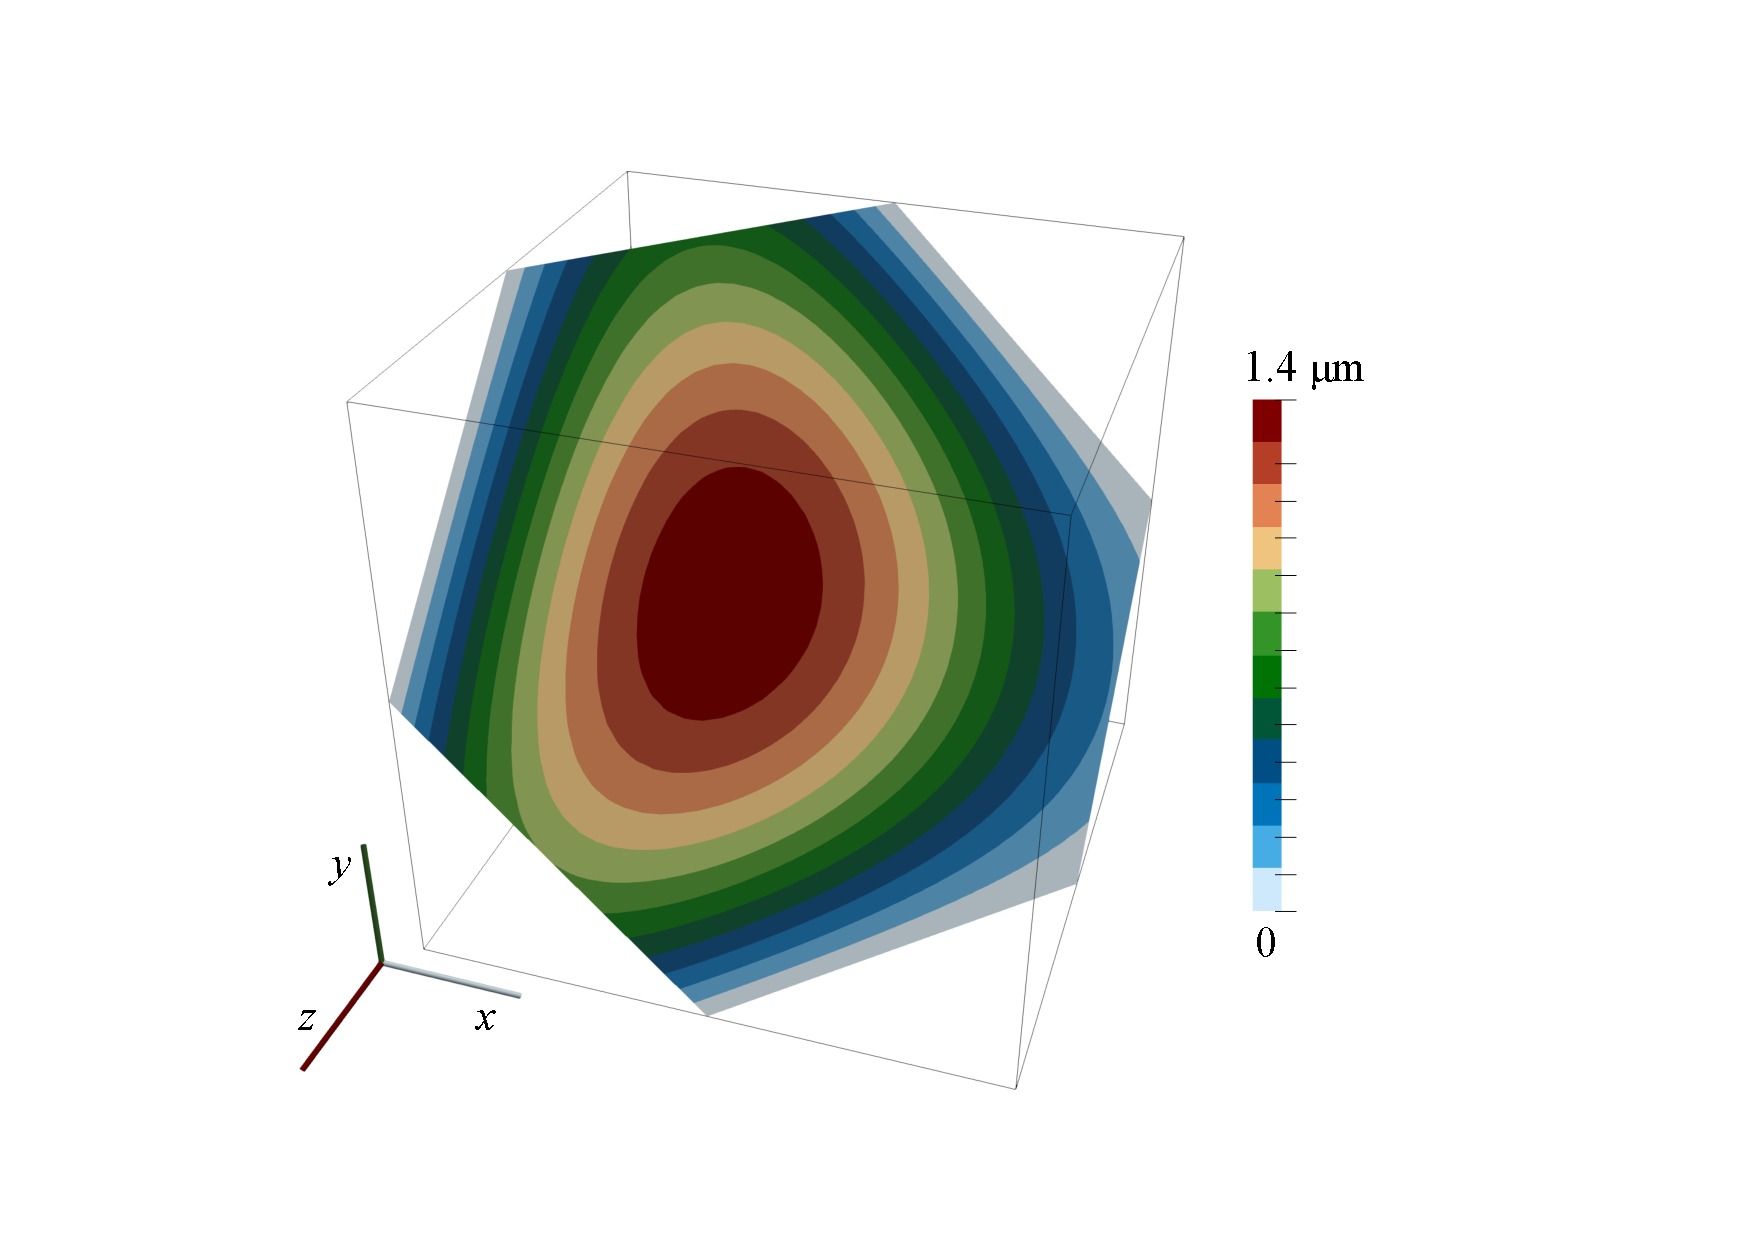
\includegraphics[width=0.5\textwidth]{figures/mms_solution} 
%   \caption{Cut plane through the cube case geometry showing the magnitude of the manufactured displacement solution. The cut plane passes through the centre of the cube and has the unit normal $\bb{n} = (\sfrac{1}{\sqrt{3}} \quad \sfrac{1}{\sqrt{3}} \quad \sfrac{1}{\sqrt{3}})$.}
%   \label{fig:mms_solution}
%\end{figure}
\begin{figure}[htbp]
	\centering
	\subfigure[Magnitude of the manufactured displacement solution]
	{
		\label{fig:mms_solution}
   		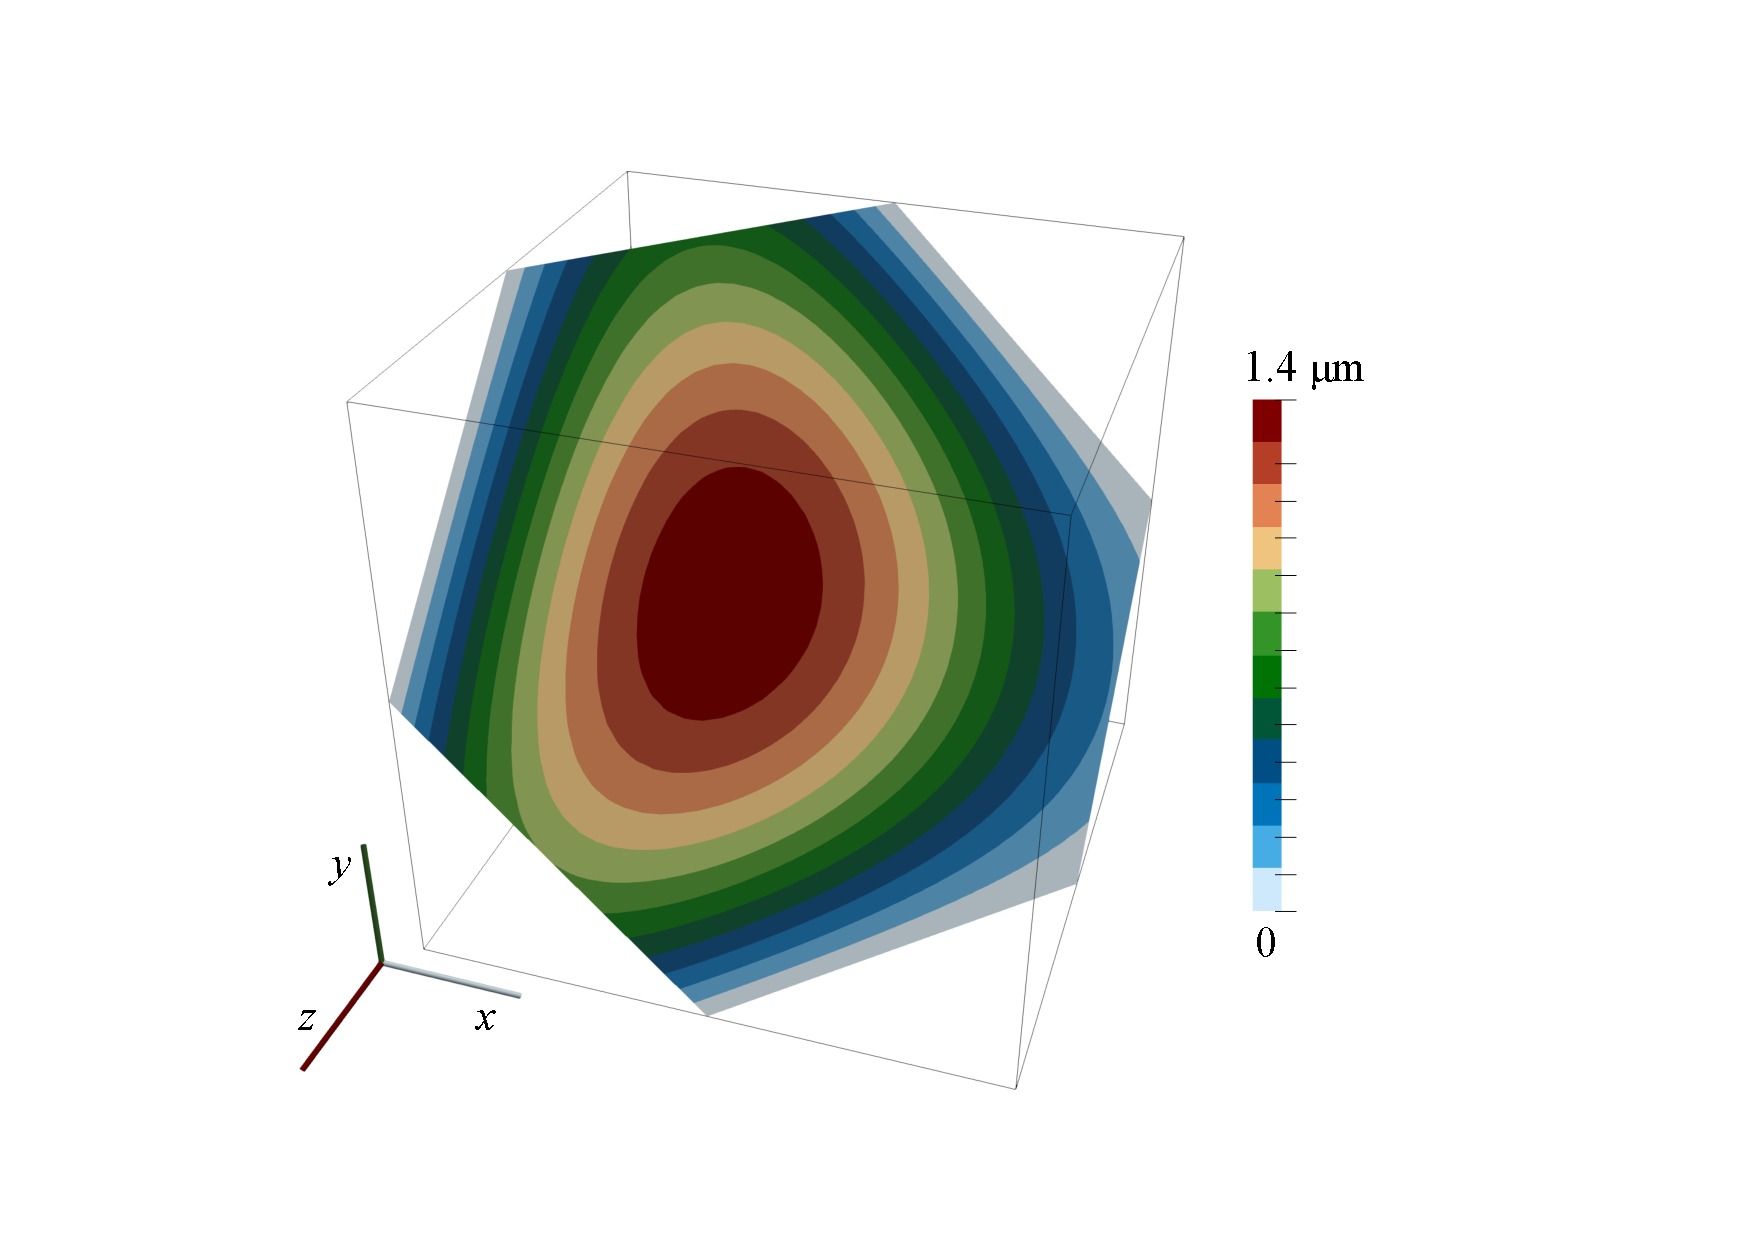
\includegraphics[height=0.45\textwidth]{figures/mms_solution} 
   	}
	\subfigure[Polyhedral mesh with $1\,000$ cells]
	{
		\label{fig:mms_mesh}
   		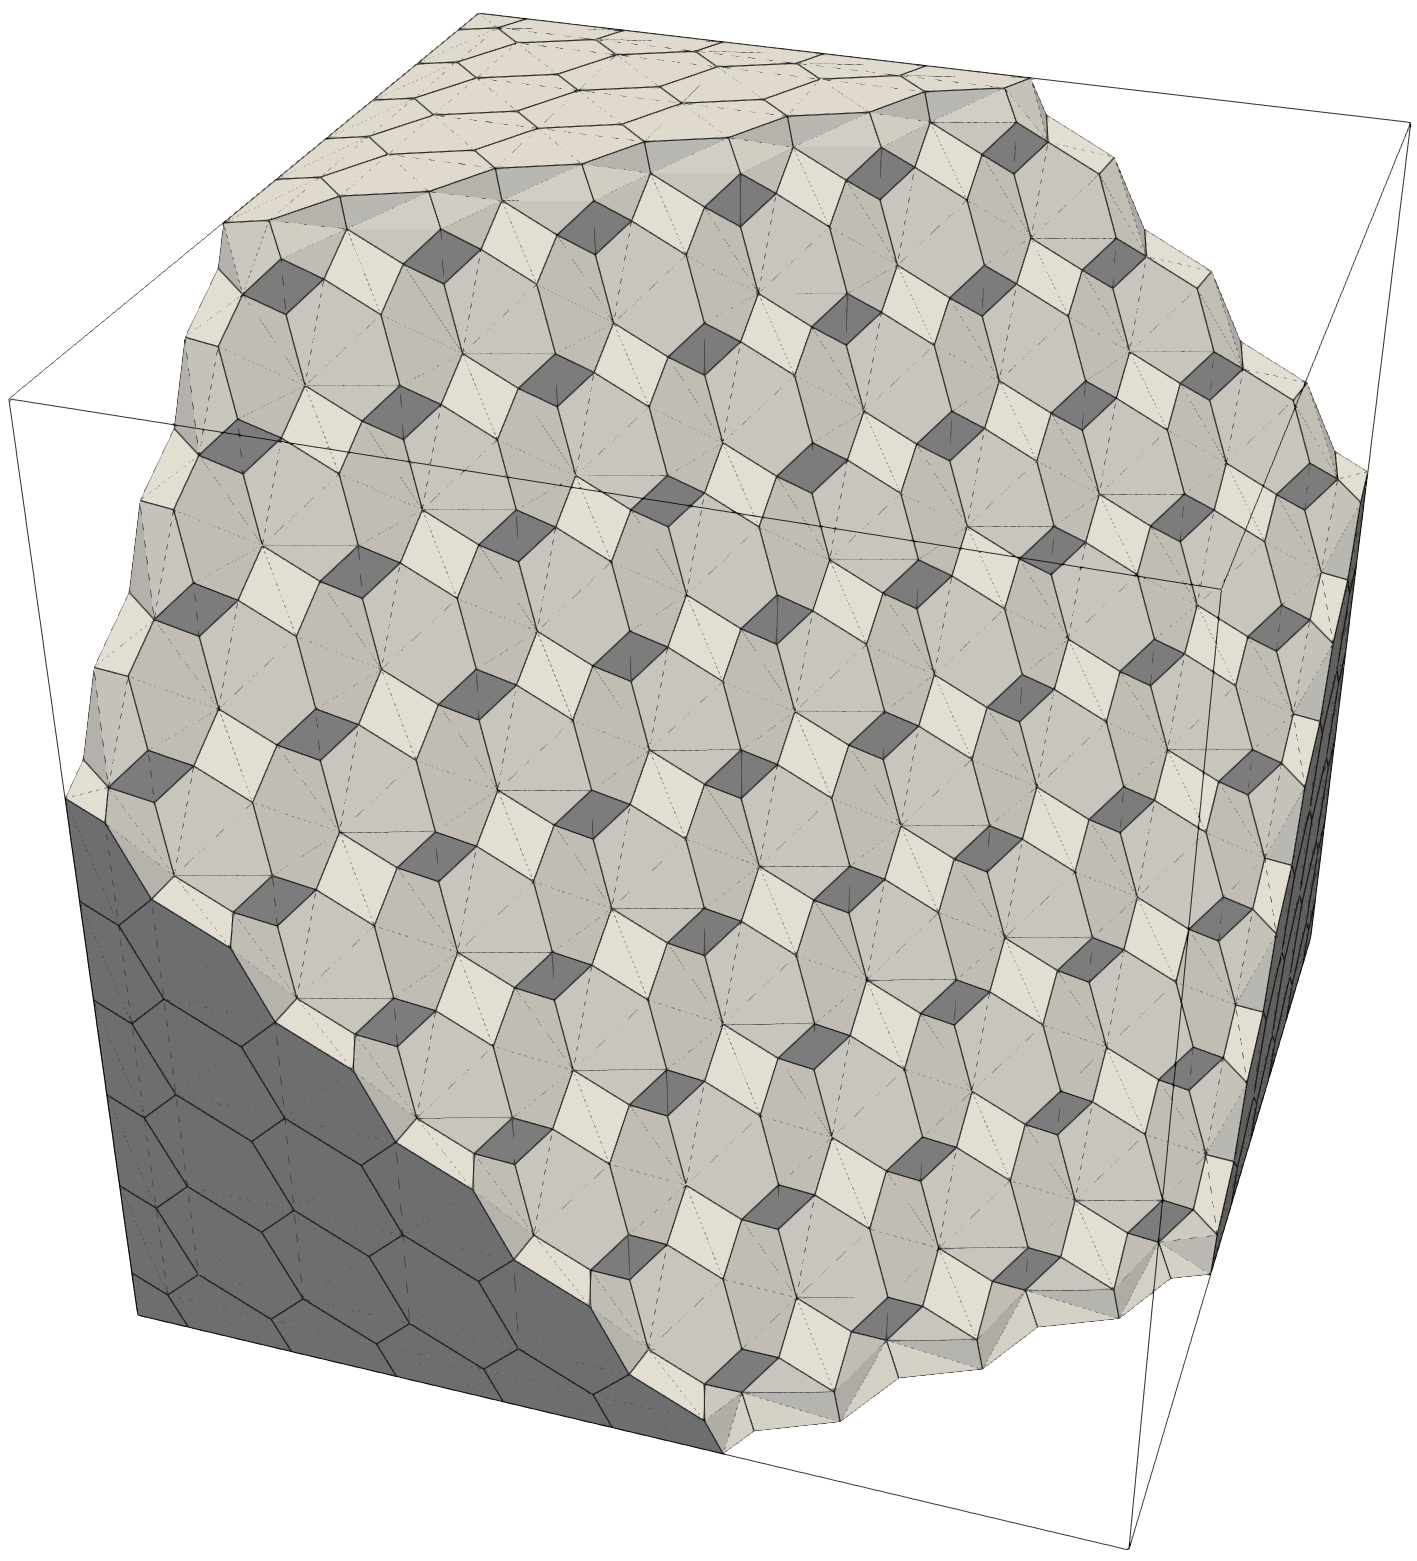
\includegraphics[height=0.45\textwidth]{figures/mms_mesh}  
   	}
	\caption{A cut plane through the cube case geometry showing the magnitude of the manufactured displacement solution (left) and a polyhedral mesh (right). The cut plane passes through the centre of the cube and has the unit normal $\bb{n} = (\sfrac{1}{\sqrt{3}} \quad \sfrac{1}{\sqrt{3}} \quad \sfrac{1}{\sqrt{3}})$.}
	\label{fig:mms}
\end{figure}

The manufactured displacement solution is applied at the domain's boundaries, and inertial effects are neglected.
Three mesh types are examined: (i) hexahedra, (ii) tetrahedra, and (iii) regular polyhedra (Figure \ref{fig:mms_mesh}).
The hexahedral meshes are created using the OpenFOAM \texttt{blockMesh} utility, while the tetrahedral meshes are created using Gmsh \citep{geuzaine2009gmsh}.
To create the polyhedral meshes, the tetrahedra meshes are converted to their dual polyhedral representations using the OpenFOAM \texttt{polyDualMesh} utility.
Starting from an initial mesh spacing of $0.04$ m, six meshes are created by successively halving the spacing.
The cell numbers for the hexahedral and polyhedral meshes are 125, $1\,000$, $8\,000$, $64\,000$, $512\,000$, and $4\,096\,000$, while the tetrahedral mesh cell counts are 384, $4\,374$, $41\,154$, $355\,914$, $2\,958\,234$, and $24\,118\,074$.
For the same average cell width, the cell counts show that the tetrahedral meshes have larger cell counts by a factor of 3 to 6.

Figure \ref{fig:mms_disp_accuracy}(a) shows the displacement magnitude discretisation errors ($L_2$ and $L_\infty$) as a function of the average cell width for all three mesh types (hexahedral, tetrahedral and polyhedral), while Figure \ref{fig:mms_disp_accuracy}(b) shows the corresponding order of accuracy plots.
For ease of interpretation, the symbol shapes in the figures have been chosen to correspond to the cell shapes: a square for hexahedra, a triangle for tetrahedra and a pentagon for polyhedra.
The maximum ($L_\infty$) and average ($L_2$) discretisation errors are seen to reduce at an approximately second-order rate for all mesh types, except for the $L_2$ error on the hexahedral meshes, which is approximately 2.3 on the finest grid.
%where, interestingly, the errors are, on average, smaller on the polyhedral meshes.
%The reason for this is unclear but may be due to the stencil of the structured polyhedra being more isotropic and containing close neighbours.
\begin{figure}[htbp]
	\centering
	\subfigure[Displacement magnitude discretisation errors]
	{
   		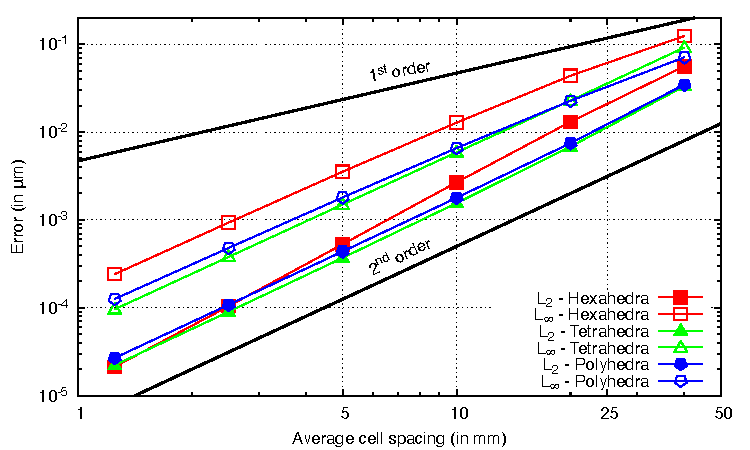
\includegraphics[width=0.45\textwidth]{figures/mms_dispErrors} 
   	}
	\subfigure[Displacement discretisation error order of accuracy]
	{
   		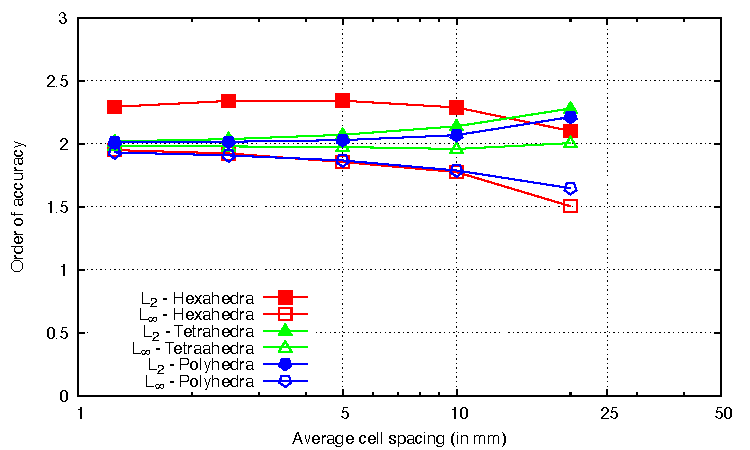
\includegraphics[width=0.45\textwidth]{figures/mms_disp_orderOfAccuracy}  
   	}
	\caption{Manufactured solution cube case: the accuracy and order of accuracy for displacement magnitude}
	\label{fig:mms_disp_accuracy}
\end{figure}

The predicted $\sigma_{xx}$ stress distribution for a hexahedral mesh with $512\,000$ cells is shown in Figure \ref{fig:mms_stress}(a).
The corresponding cell-wise $\sigma_{xx}$ error distribution is shown in Figure \ref{fig:mms_stress}(b).
The errors of greatest magnitude ($43$ kPa) occur at the boundaries, corresponding to where the local truncation error is higher due to the use of one-sided differencing.
\begin{figure}[htbp]
	\centering
	\subfigure[Predicted $\sigma_{xx}$ stress distribution]
	{
		\label{fig:mms_sxx}
   		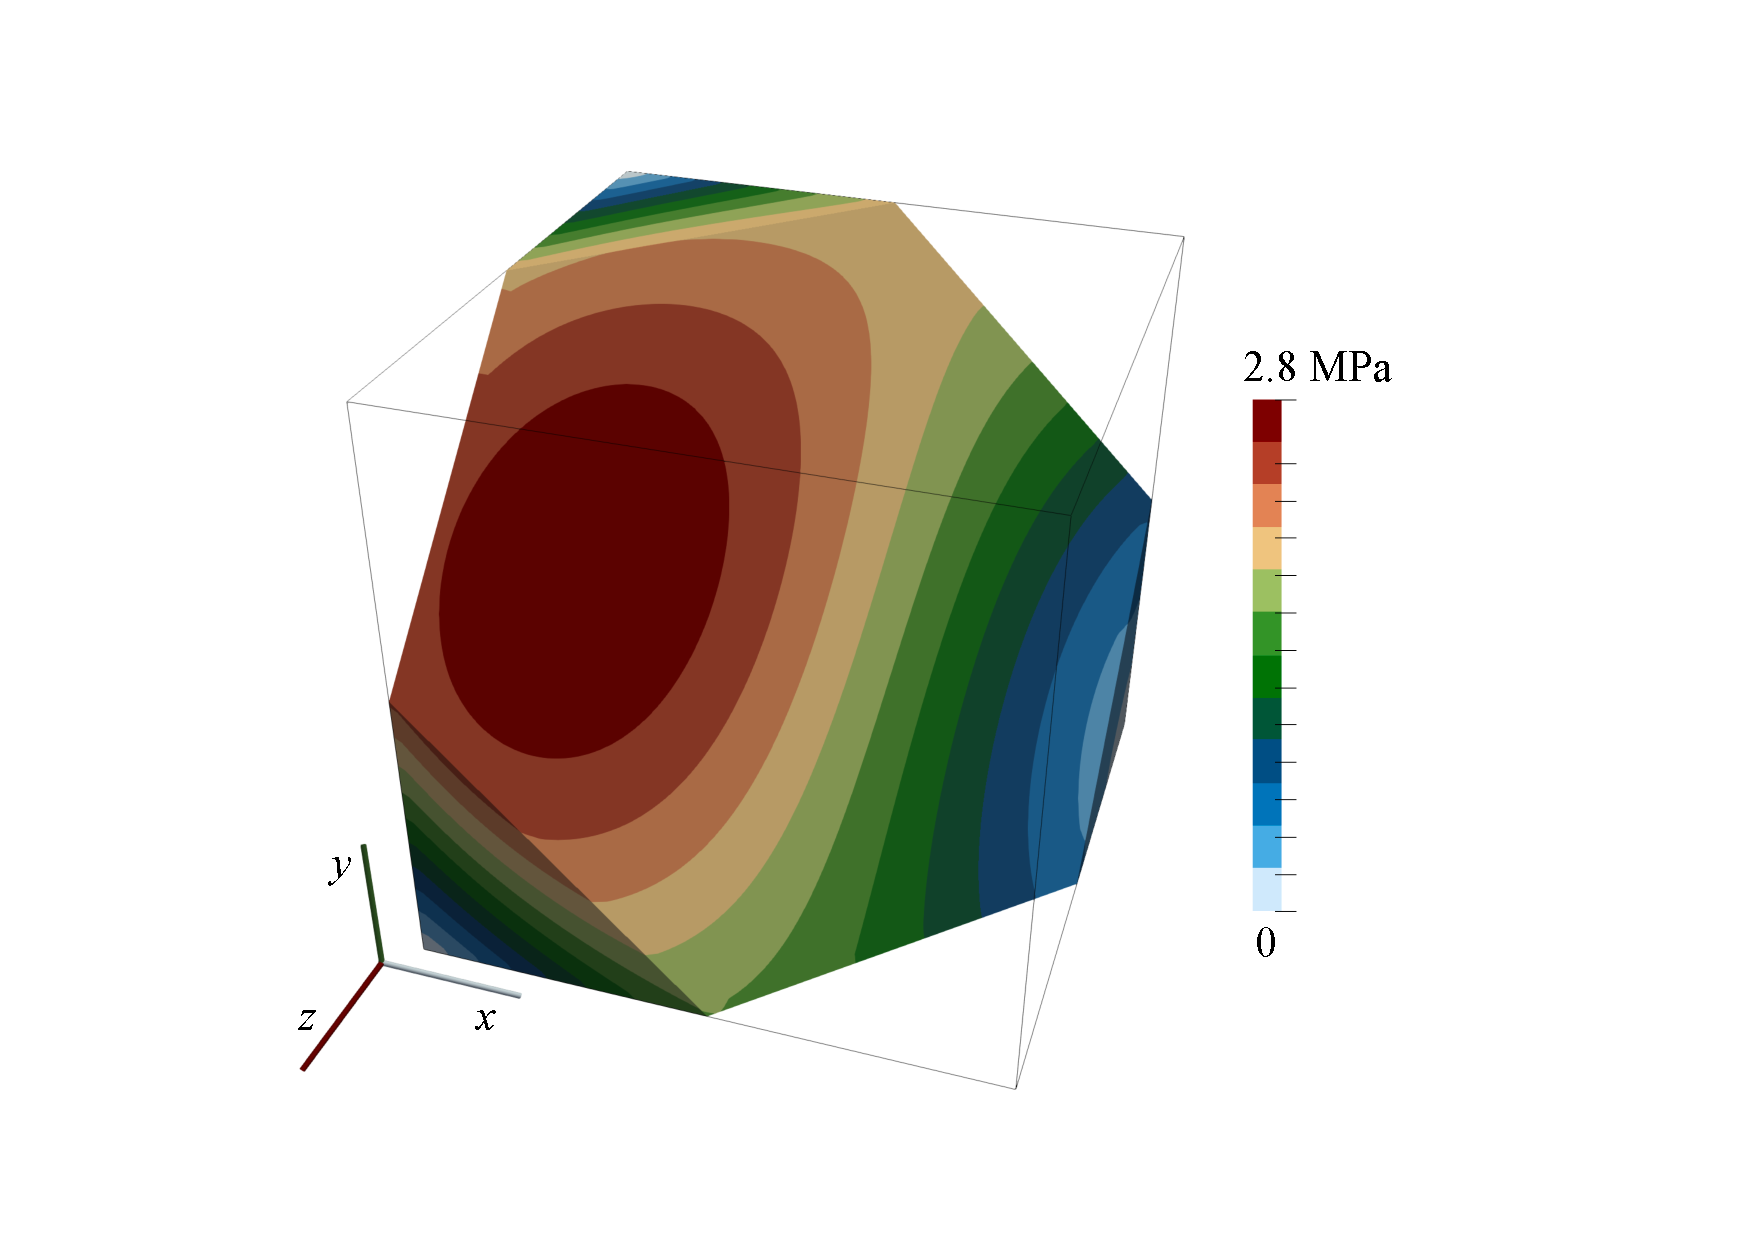
\includegraphics[height=0.35\textwidth]{figures/mms_sxx} 
   	}
	\subfigure[Cell-wise $\sigma_{xx}$ error distribution]
	{
		\label{fig:mms_sxx_diff}
   		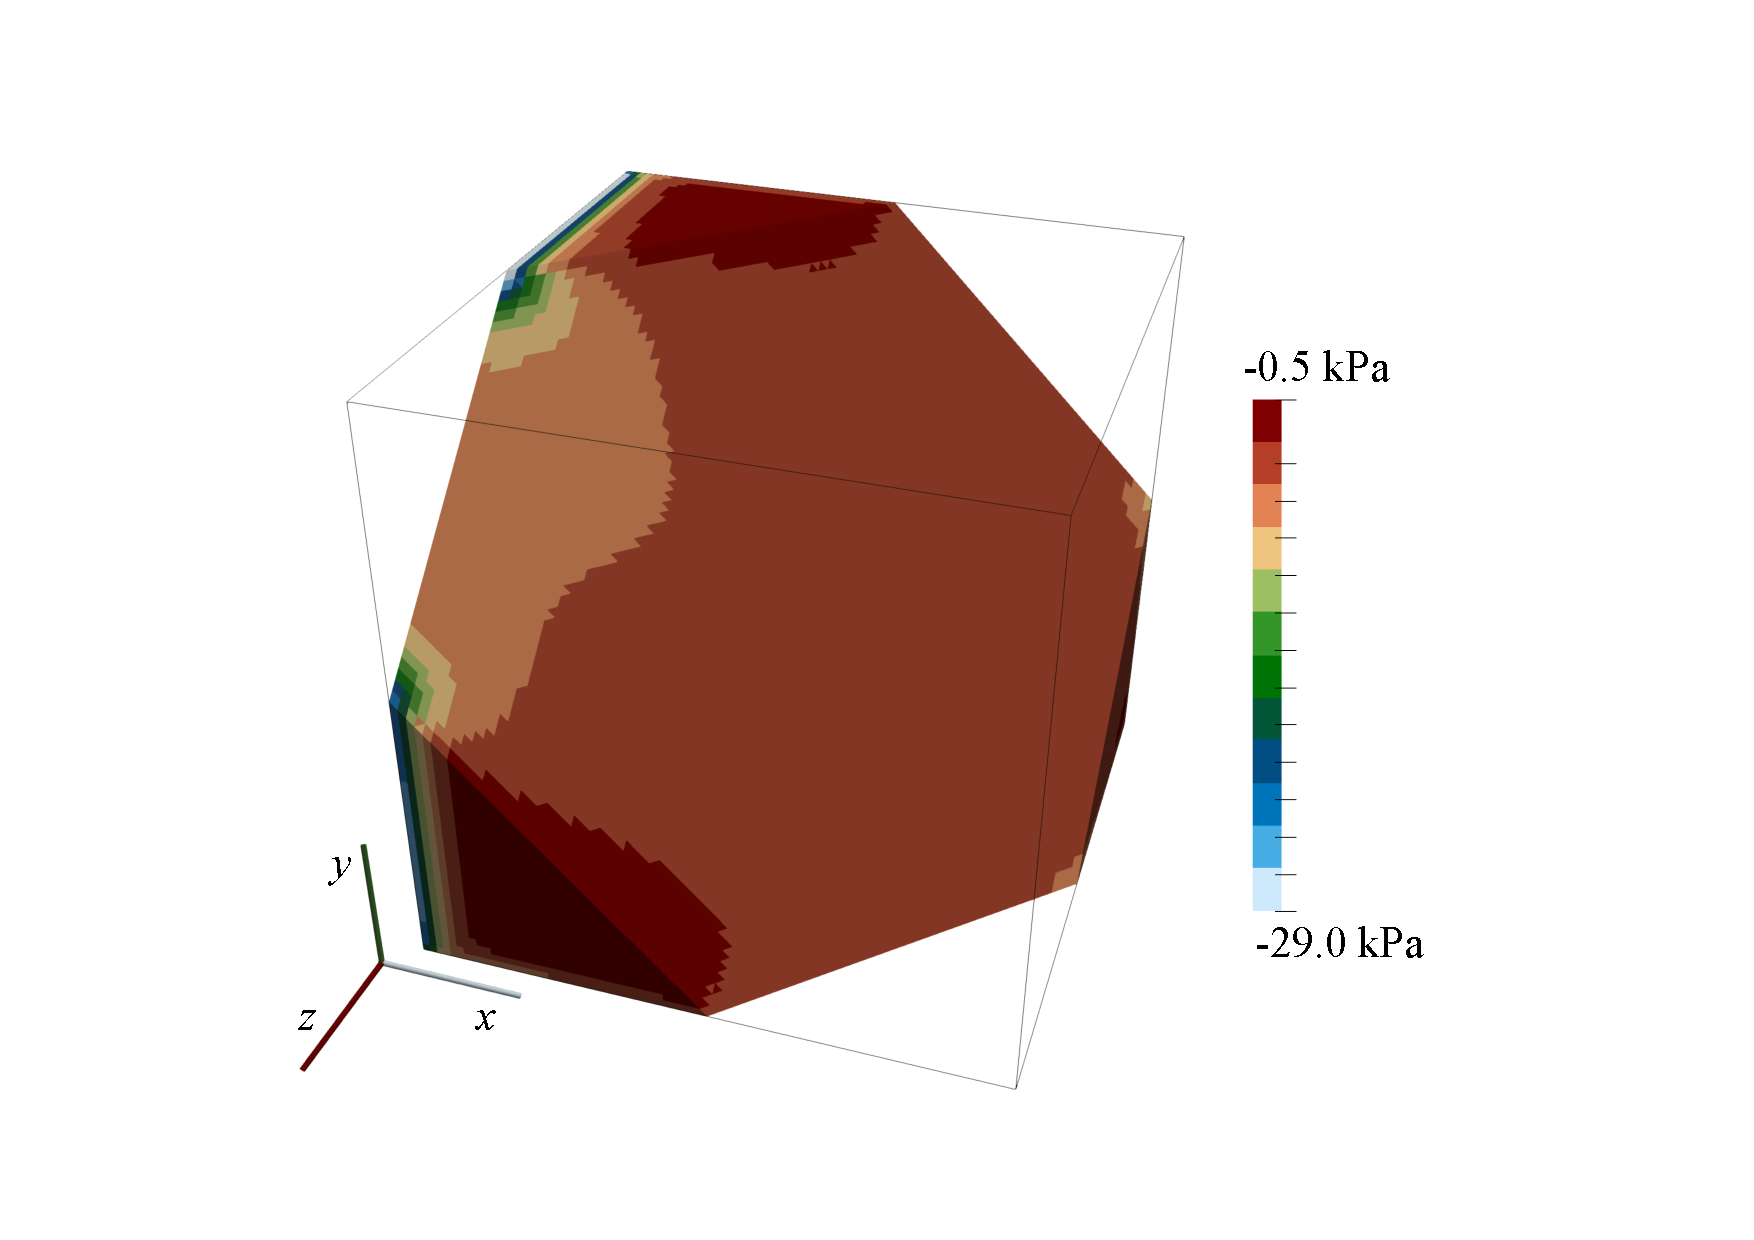
\includegraphics[height=0.35\textwidth]{figures/mms_sxx_diff}  
   	}
	\caption{Manufactured solution cube case: the predicted $\sigma_{xx}$ stress distribution on a cut-plane for the hexahedral mesh with $512\,000$ cells (left).}
	\label{fig:mms_stress}
\end{figure}
The discretisation errors in the stress magnitude are shown in Figure \ref{fig:mms_stress_accuracy}(a), and the order of accuracy in Figure \ref{fig:mms_stress_accuracy}(b).
The order of accuracy for the average ($L_2$) stress error is seen to be approximately 1.5 for the hexahedral and polyhedral meshes.
In contrast, the average stress error order for the tetrahedral meshes is 1.
Similarly, the maximum ($L_\infty$) stress order of accuracy is seen to approach 1 for all three mesh types.
\begin{figure}[htbp]
	\centering
	\subfigure[Stress magnitude discretisation errors]
	{
   		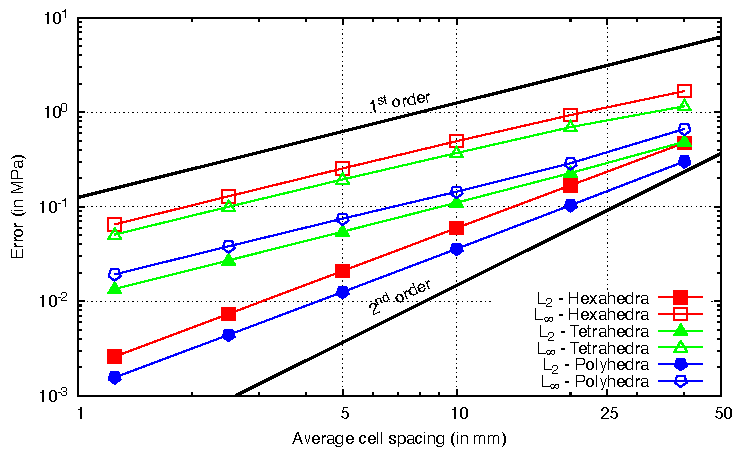
\includegraphics[width=0.45\textwidth]{figures/mms_stressErrors} 
   	}
	\subfigure[Stress discretisation error order of accuracy]
	{
   		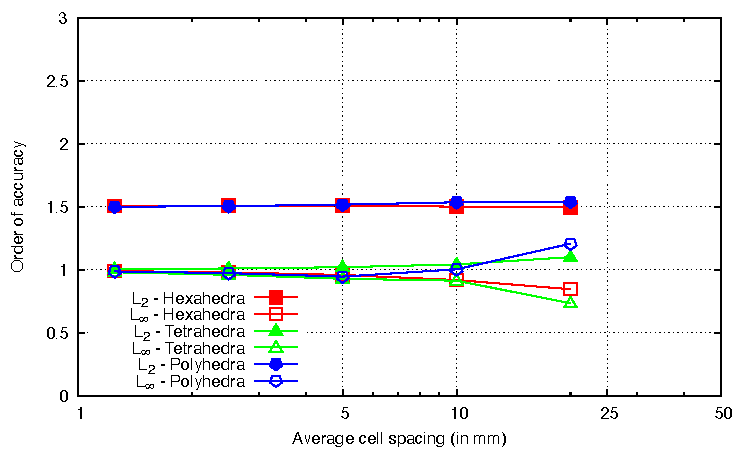
\includegraphics[width=0.45\textwidth]{figures/mms_stress_orderOfAccuracy}  
   	}
	\caption{Manufactured solution cube case: the accuracy and order of accuracy for stress magnitude}
	\label{fig:mms_stress_accuracy}
\end{figure}

The presented results have been generated using the Jacobian-free Newton-Raphson solution algorithm; however, minimal differences were seen when using the segregated solution algorithm, and hence, the segregated results are not shown.
%This section assesses the order of accuracy of the discretisation using a manufactured solution on a cube domain (case 1).
%A secondary purpose is to demonstrate that the choice of solution algorithm (Jacobian-free Newton-Krylov vs segregated) does not affect the predictions, assuming iteration errors are small.

% Note: this is PETSc segregated so discretisation is exactly the same; OF segregated will be slightly different as boundary gradients are different
% \hl{check - maybe one comparison graph}.
%\hl{Seg and JFNK are the same when including boundary values but this causes a problem for the poly grid}





\paragraph{Case 1b: Spherical Cavity in an Infinite Solid Subjected to Remote Stress}
This 3-D problem consists of a spherical cavity with radius $a = 0.2$ m (Figure \ref{fig:spherical_cavity}) in an infinite, isotropic linear elastic solid ($E = 200$ GPa, $\nu = 0.3$).
Far from the cavity, the solid is subjected to a tensile stress $\sigma_{zz} = T = 1$ MPa, with all other stress components zero.
\begin{figure}[htbp]
   \centering
   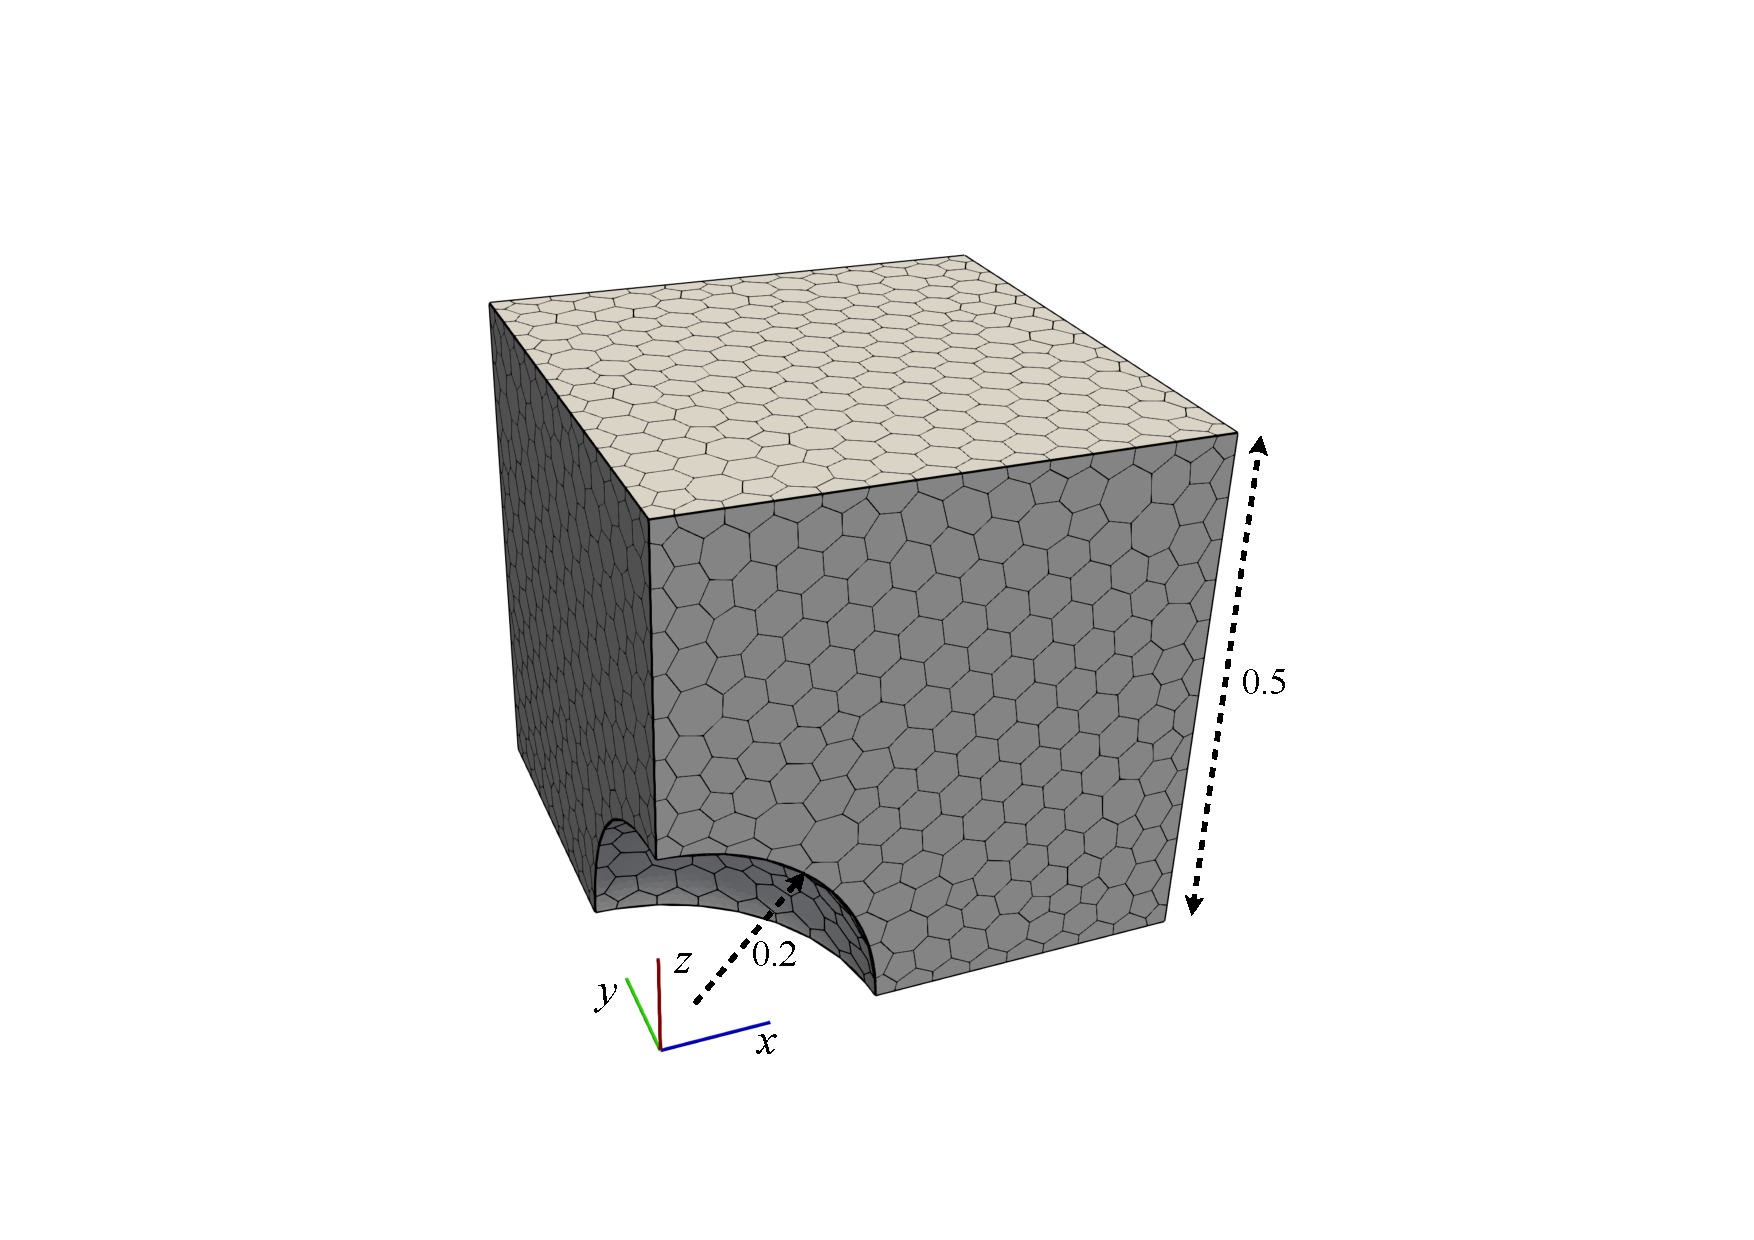
\includegraphics[width=0.4\textwidth]{figures/spherical_cavity.pdf} 
   \caption{Spherical cavity case geometry, showing the polyhedral mesh with $4\,539$}
   \label{fig:spherical_cavity}
\end{figure}
The analytical expressions for the stress and displacement distributions are given in Appendix \ref{app:sphericalCavity}.


The computational solution domain is taken as one-eighth of a $1 \times 1 \times 1$ m cube aligned with the Cartesian axes, with one corner at the centre of the sphere.
The analytical tractions are applied at the far boundaries of the domain to mitigate the effects of finite geometry.
Unstructured polyhedral meshes are employed with grading towards the cavity.
The cell sizes at the cavity surfaces are 100, 50, 25, 12.5, 6.25, and 3.125 mm, and the corresponding cell counts are 976, $4\,552$ (Figure \ref{fig:spherical_cavity}), $29\,611$, $213\,100$, $\,614\,261$.
Initially, unstructured tetrahedral meshes were generated using the Gmsh meshing utility \cite{geuzaine2009gmsh}, followed by conversion to their dual polyhedral representations using the OpenFOAM \texttt{polyDualMesh} utility.

\hl{The spherical cavity case errors seem to approach zero order accuracy}
\hl{Maybe we have hit the precision limit...?}
\hl{We may leave this case out}


\paragraph{Case 2: Out-of-plane bending of an elliptic plate}
This 3-D, static, linear elastic test case (Figure \ref{fig:elliptic_plate}) consists of a thick elliptic plate (0.6 m thick) with a centred elliptic hole, with the inner and outer ellipses given as
\begin{eqnarray}
	\left(\frac{x}{2}\right)^2 + \left(\frac{y}{1}\right)^2 = 1 & \text{inner ellipse} \\
	\left(\frac{x}{3.25}\right)^2 + \left(\frac{y}{2.75}\right)^2 = 1 & \text{outer ellipse}
\end{eqnarray}
The case has been described by the National Agency for Finite Element Methods and Standards (NAFEMS) \cite{Hitchings1987}, and analysed using finite volume procedures by \citet{Demirdzic1997a} and \citet{Cardiff2016a}.
Symmetry allows one-quarter of the geometry to be simulated.
A constant pressure of 1 MPa is applied to the upper surface, and the outer surface is fully clamped.
The mechanical properties are: $E = 210$ GPa, $\nu = 0.3$.
Six successively refined hexahedral meshes are used, with cell counts of 45, 472 (Figure \ref{fig:elliptic_plate}), $4\,140$, $34\,968$, $287\,280$ and $2\,438\,242$.
\begin{figure}[htbp]
   \centering
%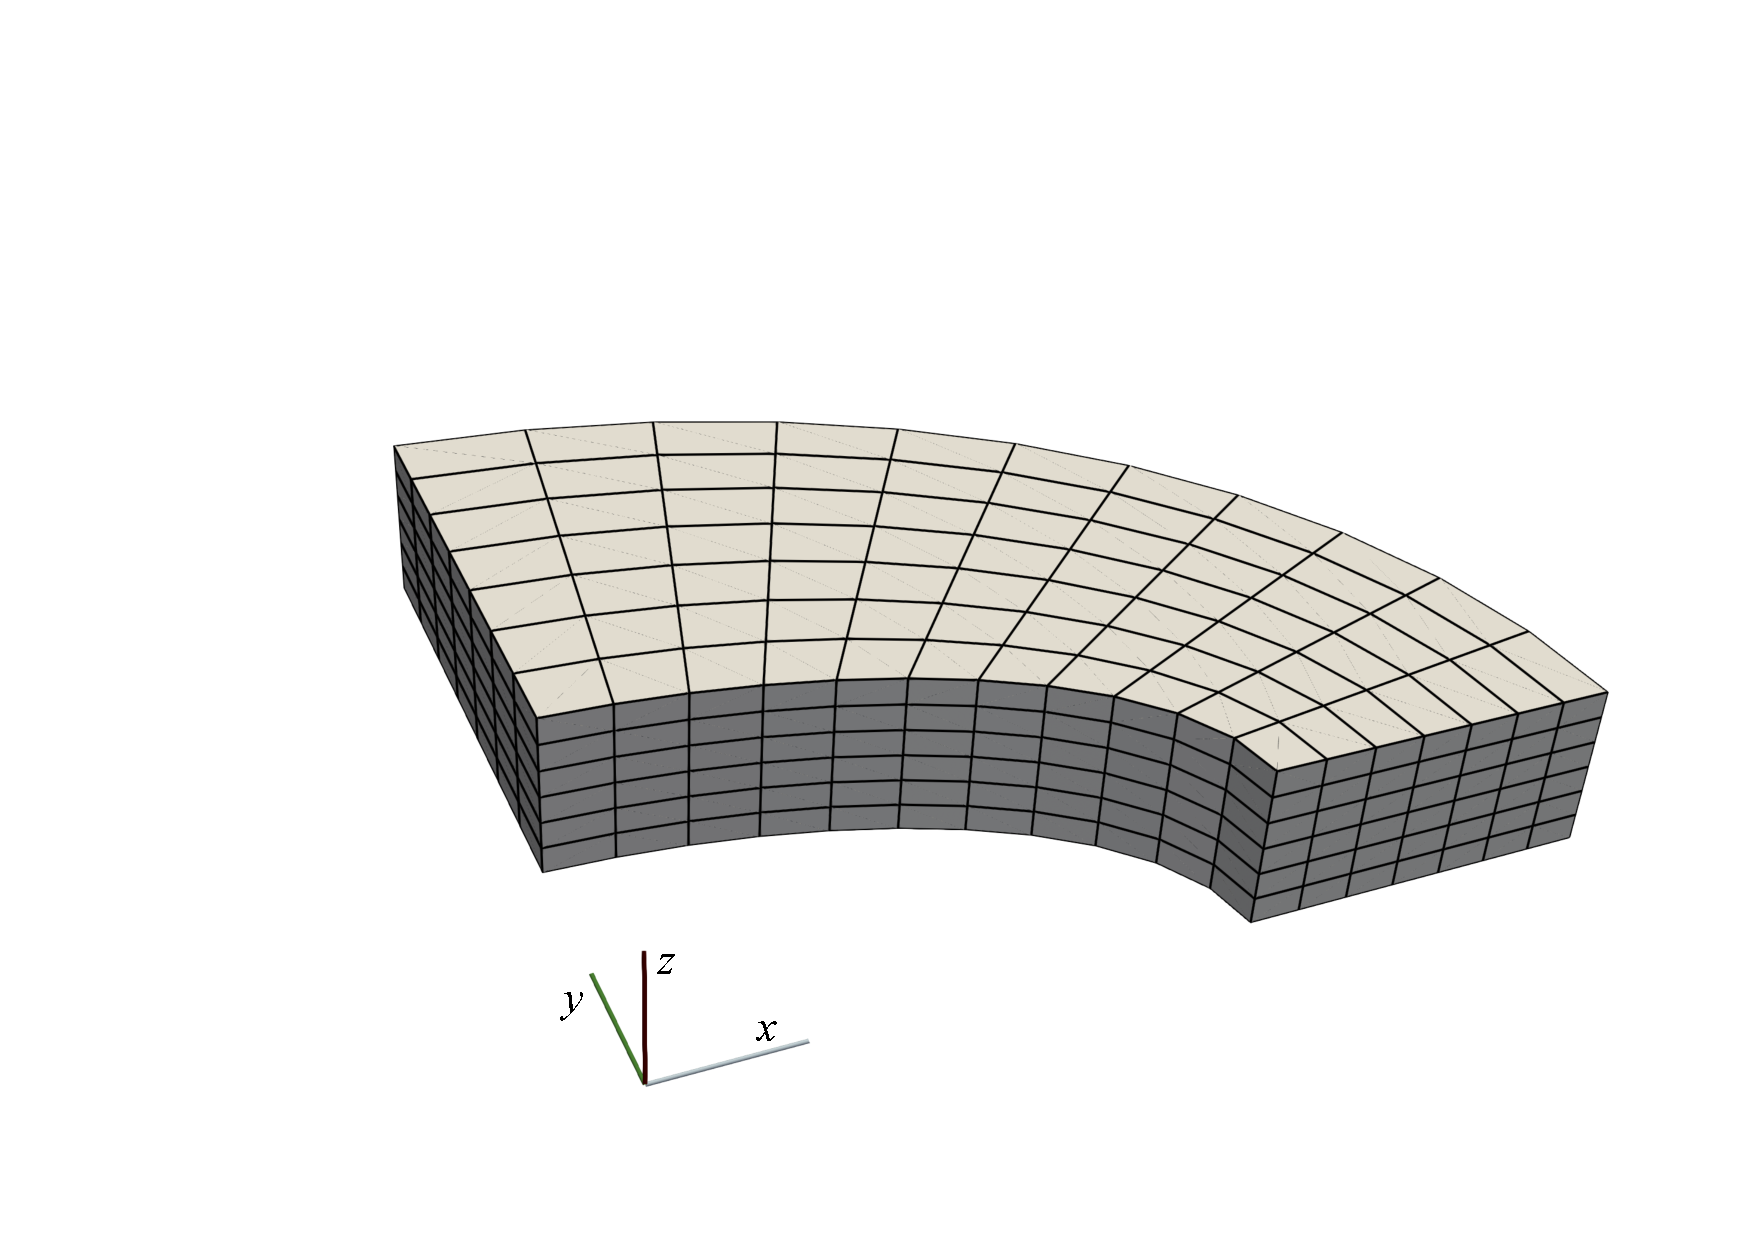
\includegraphics[width=0.5\textwidth]{figures/elliptic_plate.pdf} ellipticPlate-geometry
%	\subfigure[Mesh containing 472 hexahedral cells]
%	{
		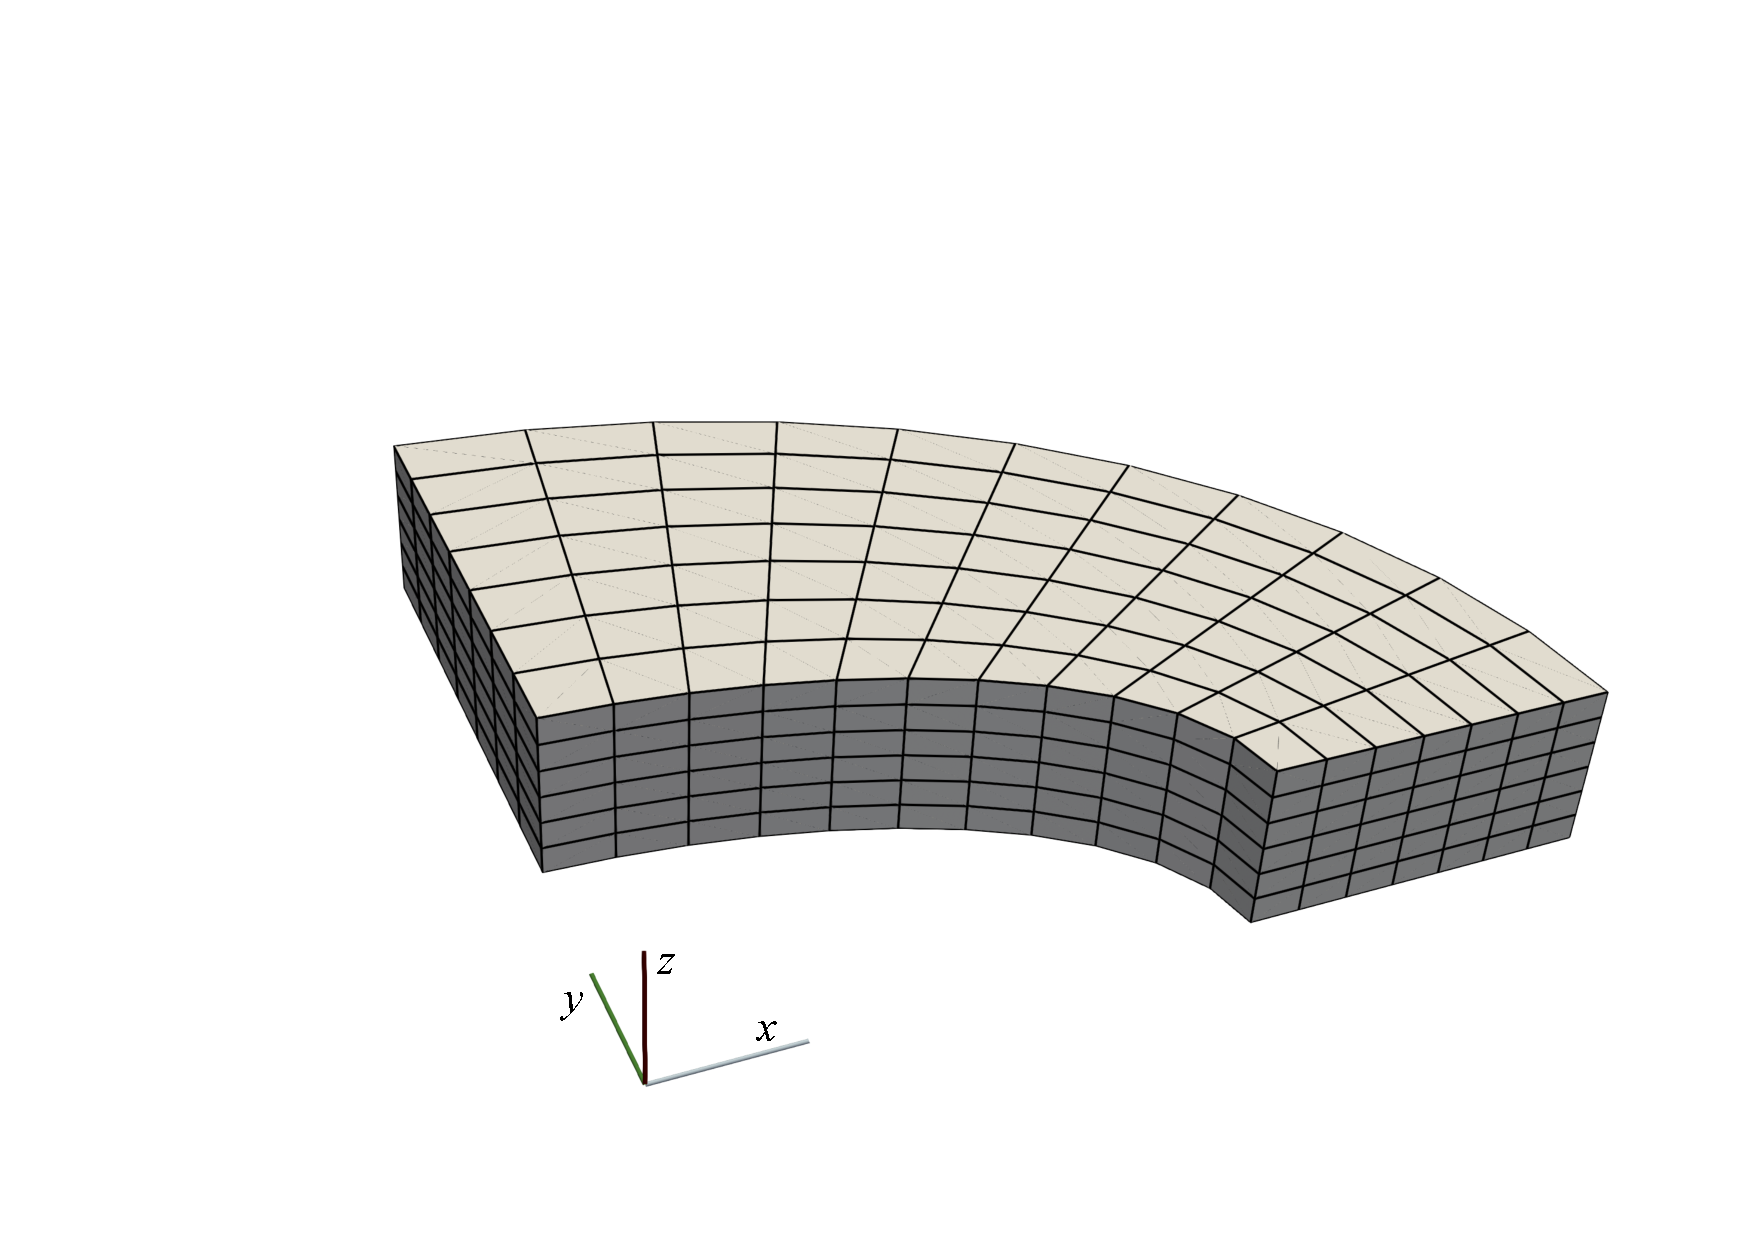
\includegraphics[width=0.45\textwidth]{figures/elliptic_plate.pdf} 
%	}
   \caption{Elliptic Plate geometry and mesh containing 472 hexahedral cells}
   \label{fig:elliptic_plate}
\end{figure}

The predictions for the equivalent (von Mises) stress along the line $r = \sqrt{x^2 + y^2} = 2.1$ m, $z = 0.3$ m is shown in Figure \ref{fig:elliptic_plate_sigmaEq}.
The results from the finest grid in \citet{Demirdzic1997a} are given for comparison, where good agreement is seen;
the small offset between the finest mesh predictions and those from \citet{Demirdzic1997a} are likely due to errors introduced when extracting the \citet{Demirdzic1997a} results using WebPlotDigitizer \citep{WebPlotDigitizer}.
The sample values have been calculated by generating 40 uniformly spaced angles between 0 and $\frac{\pi}{2}$ along the line, finding the cell of each sampled point, and extrapolating from the cell-centred value using the field gradient.
\begin{figure}[htbp]
   \centering
   %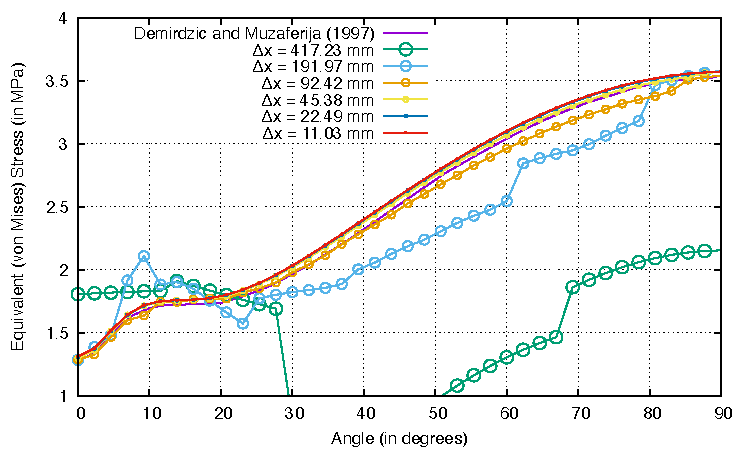
\includegraphics[width=0.5\textwidth]{figures/elliptic_plate_sigmaEq_line.pdf} 
	\subfigure[Equivalent stress distribution for the mesh with $2\,438\,242$ cells. The deformation is scaled by $1\,000$ and a translucent line indicates the outline of the undeformed geometry]
	{
		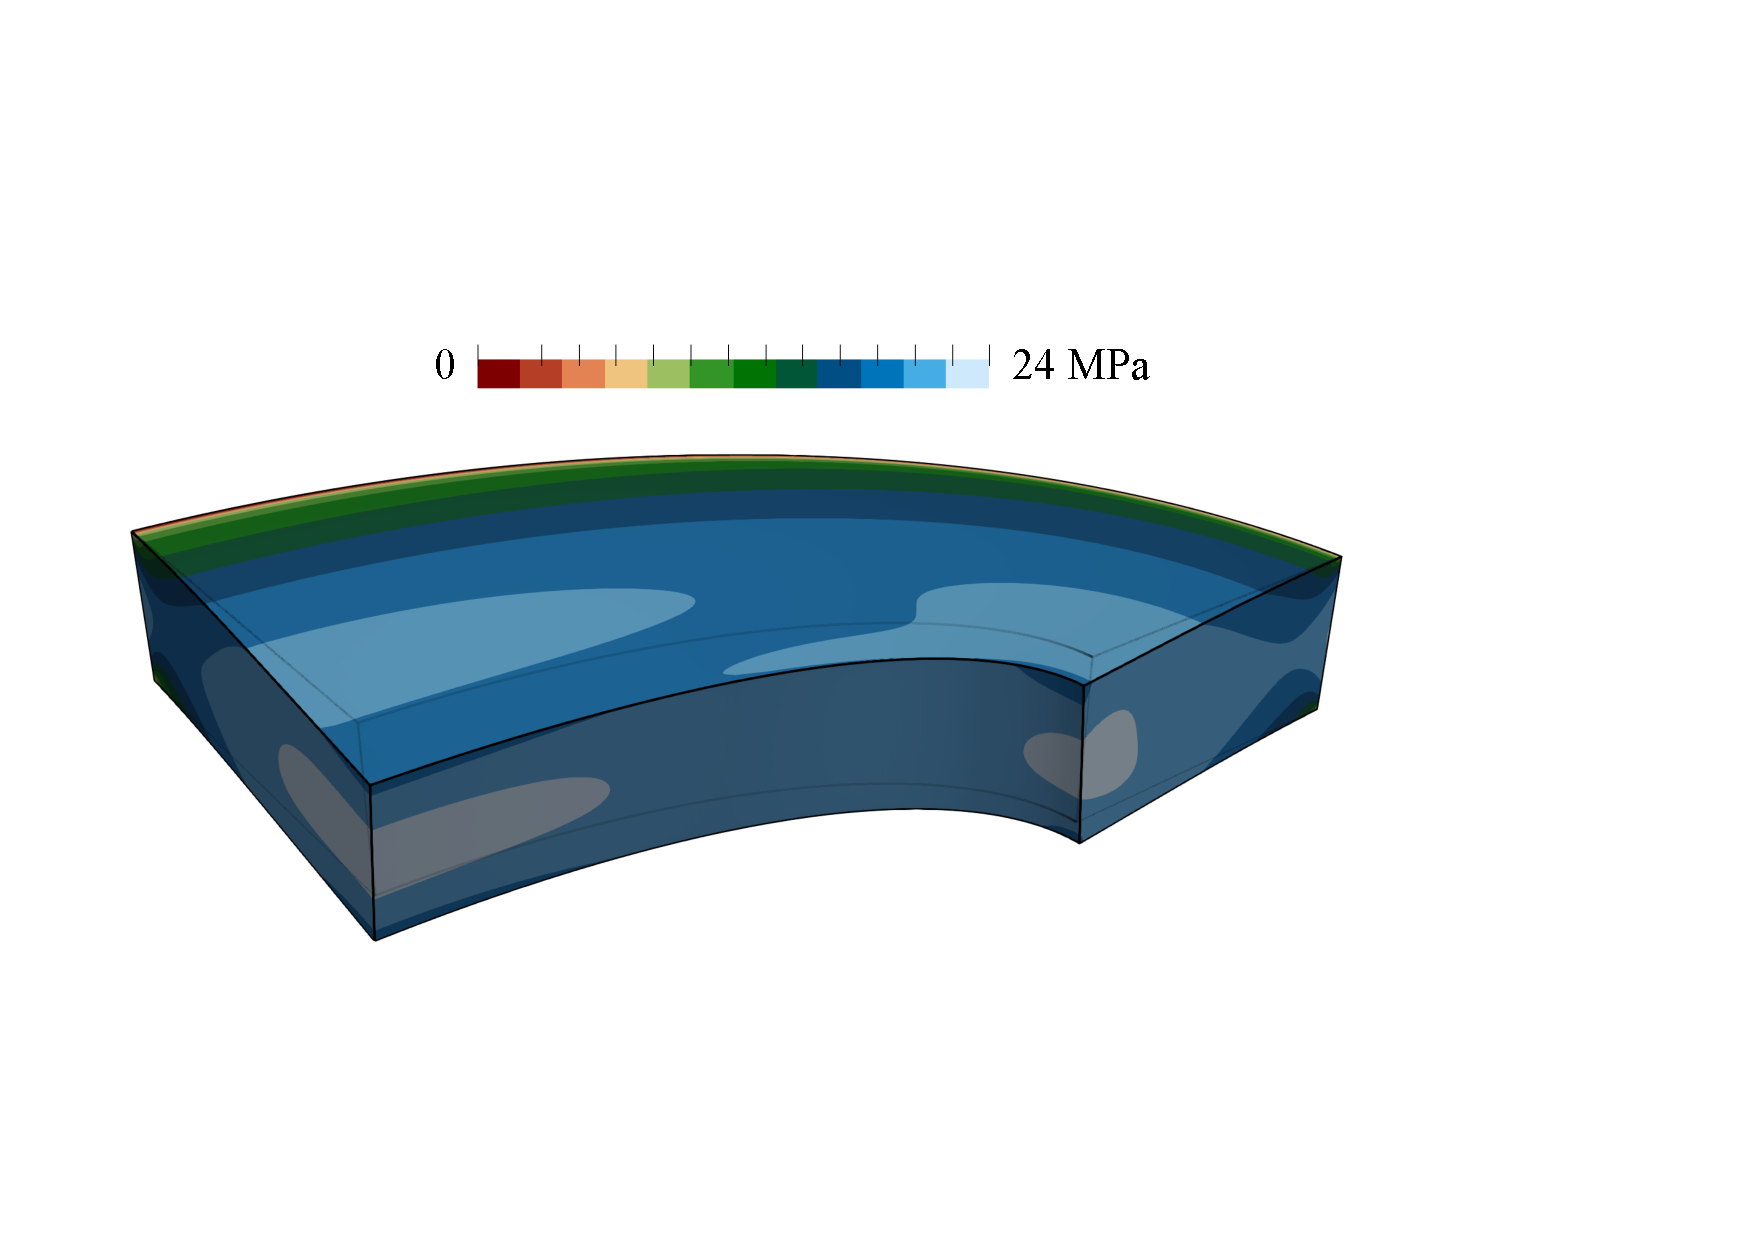
\includegraphics[width=0.45\textwidth]{figures/elliptic_plate_sigmaEq}  
	}
	\subfigure[Equivalent stress along the line $r = 2.1$, $z = 0.3$ m]
	{
		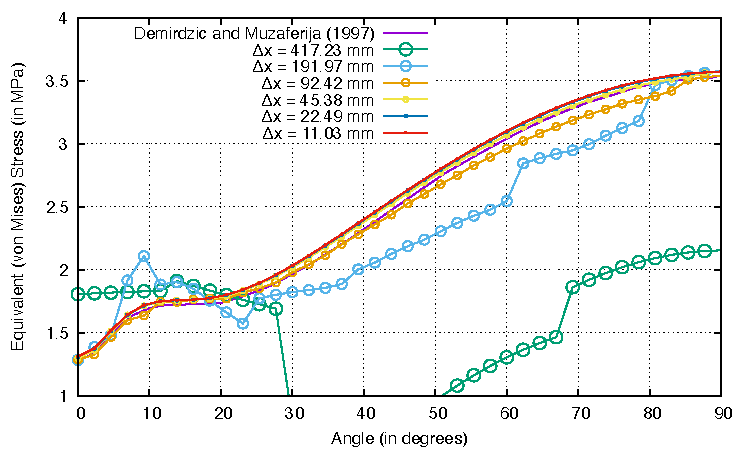
\includegraphics[width=0.45\textwidth]{figures/elliptic_plate_sigmaEq_line.pdf} 
	}
   \caption{Equivalent (von Mises) stress distribution in the elliptic plate}
   \label{fig:elliptic_plate_sigmaEq}
\end{figure}


\paragraph{Case 3: Narrow T-section component under tension}
This case, proposed by \citet{Demirdzic1997a}, consists of a narrow engineering component with a T cross-section (Figure \ref{fig:narrowTmember}).
The case is 3-D, static, with linear elastic material behaviour.
Symmetry allows one-quarter of the geometry to be simulated.
A constant negative pressure of 1 MPa is applied to the lower surface, and the upper left surface is fully clamped.
The Young’s modulus is $E = 210$ GPa, and Poisson’s ratio is $\nu = 0.3$.
A radius $5$ mm hole is located at the expected stress concentration.
%\begin{figure}[htbp]
%   \centering
%   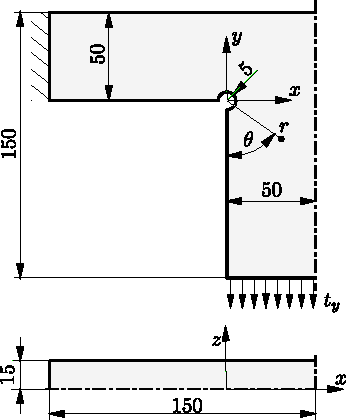
\includegraphics[width=0.4\textwidth]{figures/narrowTmember-geometry.pdf} 
%   \caption{Inflation of an idealised ventricle case geometry, mesh and loading conditions}
%   \label{fig:narrowTmember}
%\end{figure}
\begin{figure}[htbp]
	\centering
	\subfigure[Case geometry (considered quarter geometry)]
	{
		\label{fig:narrowTmember_geometry}
   		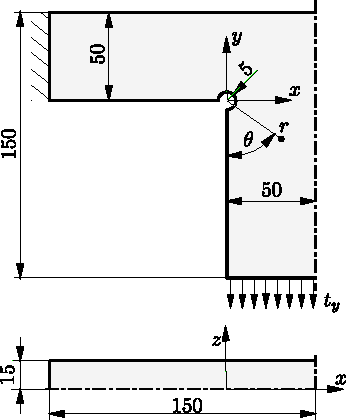
\includegraphics[height=0.4\textwidth]{figures/narrowTmember-geometry} 
   	}
   	\qquad
	\subfigure[Mesh with 624 cells]
	{
		\label{fig:narrowTmember_mesh}
   		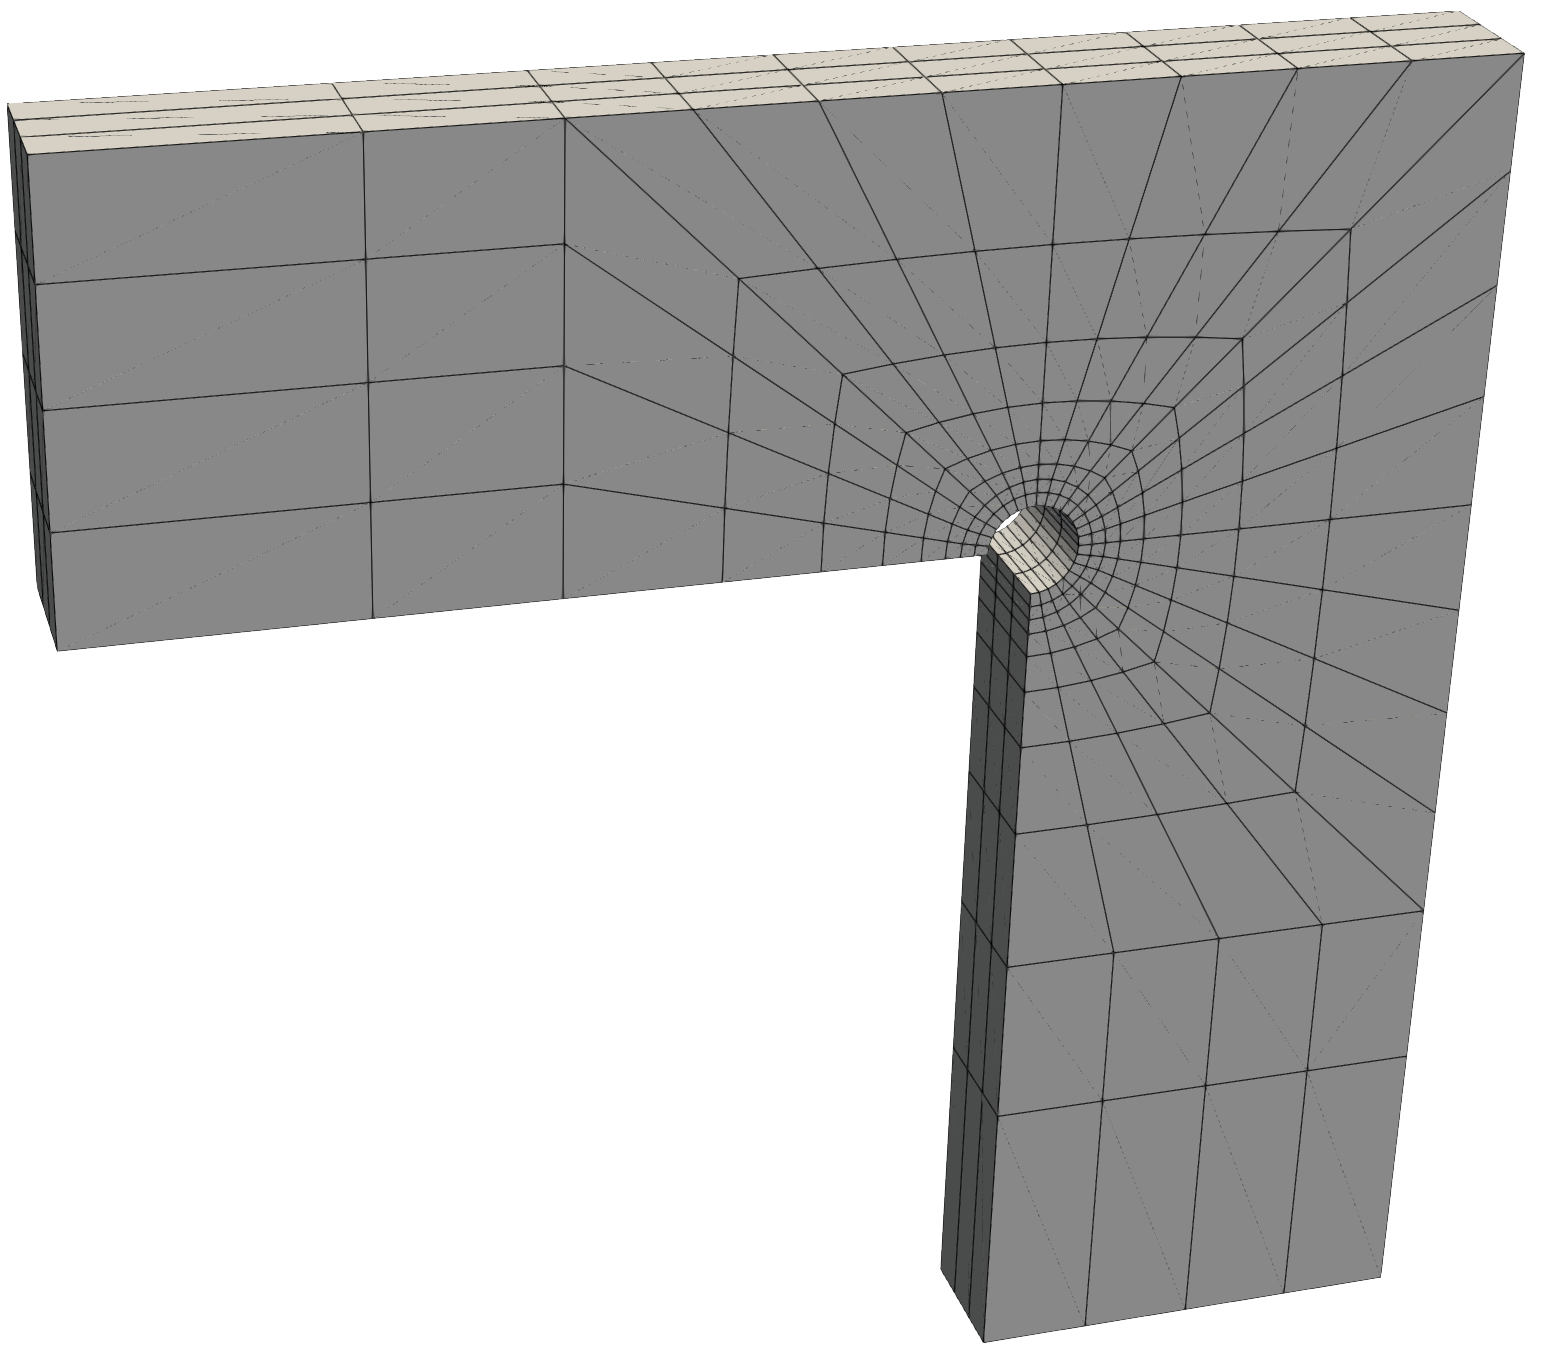
\includegraphics[height=0.4\textwidth]{figures/narrowTmember-mesh}  
   	}
	\caption{Narrow T-section component under tension: geometry and mesh}
	\label{fig:narrowTmember}
\end{figure}

Five succesively refined hexahedral meshes are created using the OpenFOAM \texttt{blockMesh} utility, consisting of 624, $4\,992$, $39\,936$, $319\,488$, and $2\,555\,904$ cells.
The corresponding average cell widths—calculated as the cubed root of the total domain volume divided by the number of cells—are 6.69, 3.34, 1.67, 0.84, and 0.42 mm.


The predicted equivalent (von Mises) stress distribution on the $z = 0$ plane is shown in Figure \ref{fig:narrowTmember_sigmaEq}(a), where a stress concentration is apparent near the hole.
The equivalent stress along the line $r = 1.5R$, $z = 0$ is shown for the different meshes in Figure \ref{fig:narrowTmember_sigmaEq}(b), where $R$ is the hole radius.
The predictions are seen converge to the results reported in \citet{Demirdzic1997a}.
Similarly to the elliptic plate case, the sample values have been to by generating 30 uniformly spaced angles between $-\frac{\pi}{2}$ and $-\pi$ along the line, finding the cell of each sampled point, and extrapolating from the cell-centred value using the field gradient.
\begin{figure}[htbp]
   \centering
	\subfigure[Equivalent stress distribution for the mesh with $2\,555\,904$ cells on the $z = 0$ m plane]
	{
		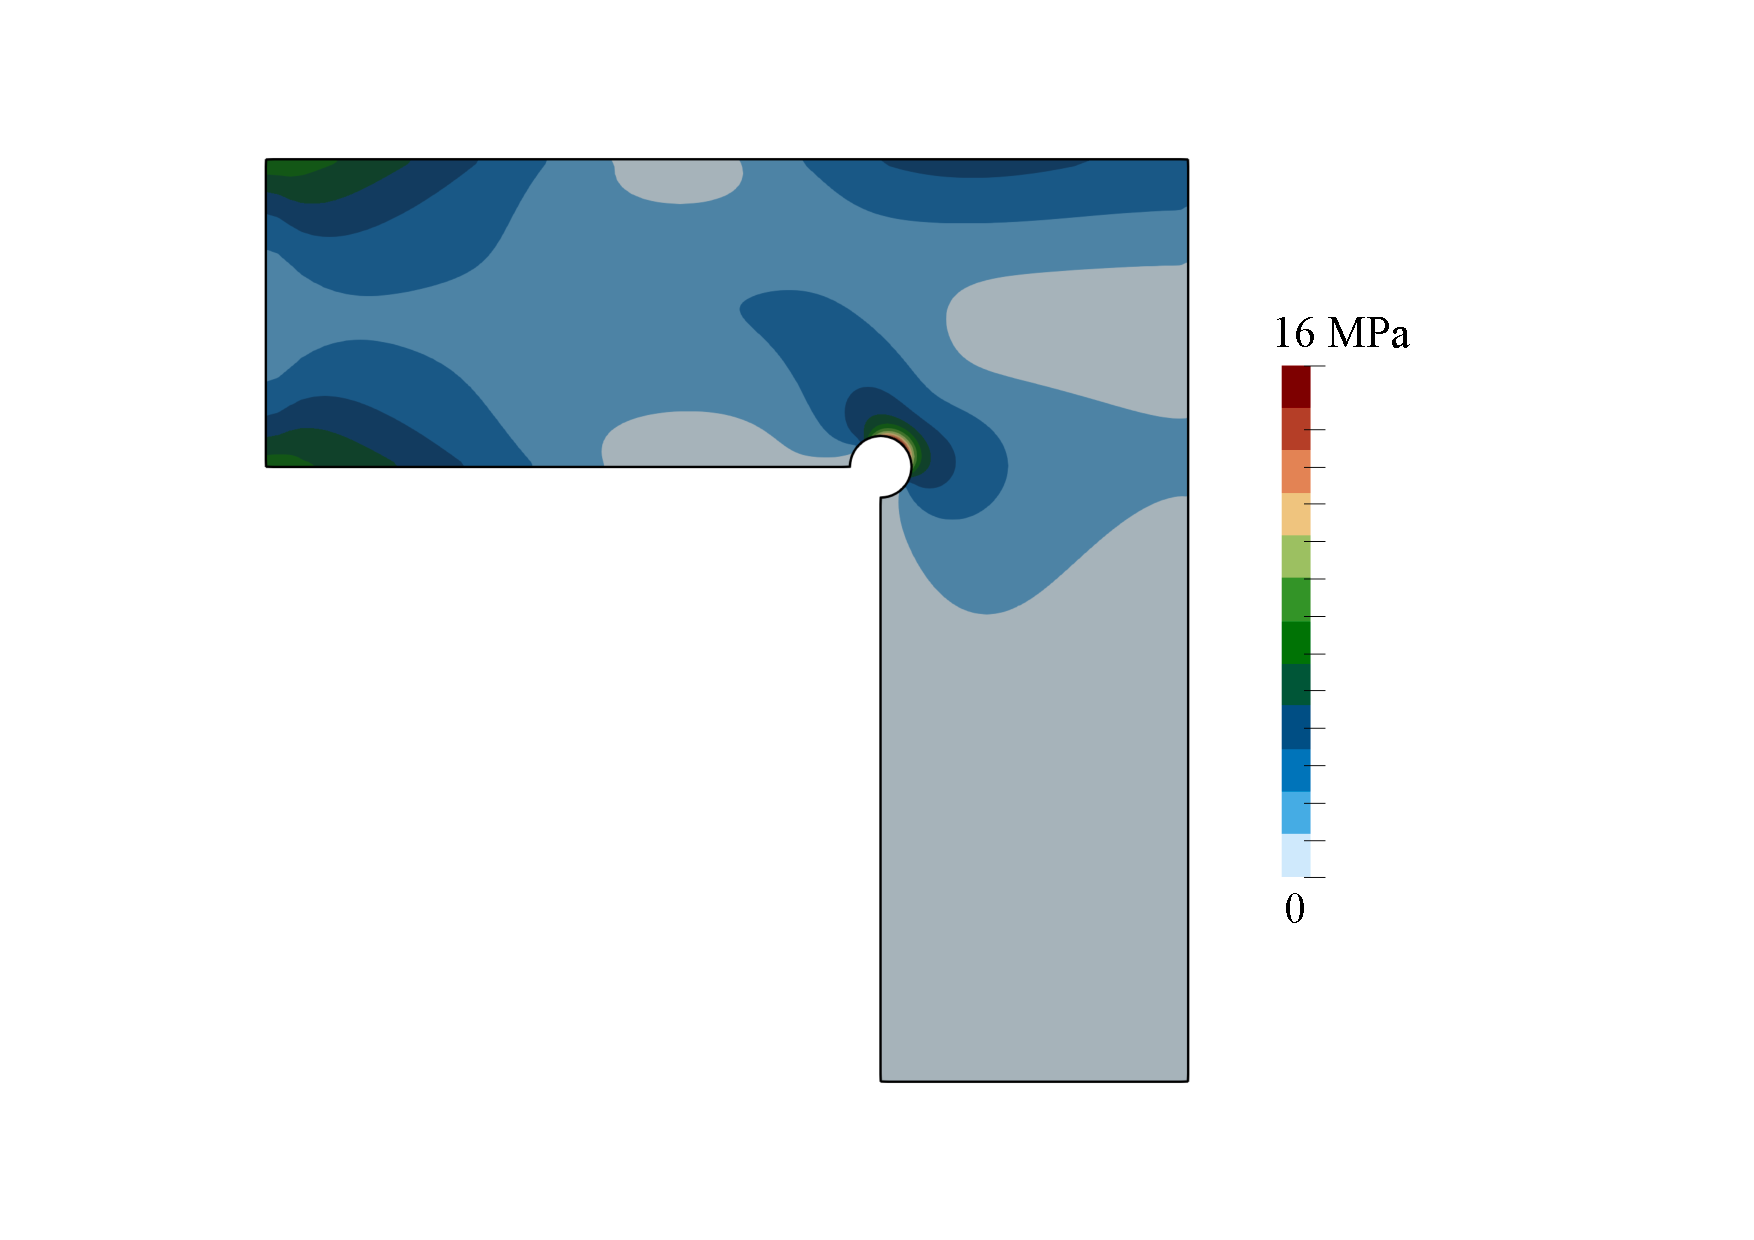
\includegraphics[height=0.32\textwidth]{figures/narrowTmember_sigmaEq}  
	}
	\subfigure[Equivalent stress along the line $r = 1.5R$, $z = 0$ m]
	{
		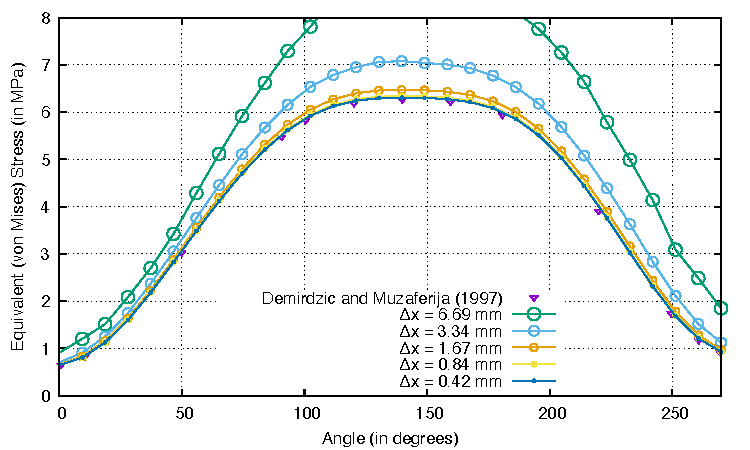
\includegraphics[height=0.32\textwidth]{figures/narrowTmember_sigmaEq_line.pdf} 
	}
   \caption{Equivalent (von Mises) stress distribution in the narrow T-section component under tension}
   \label{fig:narrowTmember_sigmaEq}
\end{figure}



\paragraph{Case 4: Inflation of an idealised ventricle}
Inflation of an idealised ventricle (Figure \ref{fig:ventricle}) was proposed by \citet{Land2015} as a benchmark problem for cardiac mechanics software.
The case is 3-D, static, with finite hyperelastic strains.
The initial geometry is defined as a truncated ellipsoid:
\begin{eqnarray}
	x = r_s \sin(u) \cos(v), \quad
	y = r_s \sin(u) \sin(v), \quad
	z = r_l \cos(u)
\end{eqnarray}
where on the inner (endocardial) surface $r_s =7$ mm, $r_l = 17$ mm, $u \in \left[-\pi, -\arccos \left( \frac{5}{17} \right) \right]$ and $v \in \left[-\pi, \pi \right]$, while on the outer (epicardial) surface $r_s =10$ mm, $r_l = 20$ mm, $u \in \left[-\pi, -\arccos \left( \frac{5}{20} \right) \right]$ and $v \in \left[-\pi, \pi \right]$.
The base plane $z = 5$ mm is implicitly defined by the ranges for $u$.
%Constitutive parameters: isotropic, 
The hyperelastic material behaviour is described by the transversely isotropic constitutive proposed by \citet{Guccione1995} law, where the parameters are $C = 10$ kPa, $b_f = b_t = b_{fs} = 1$.
The benchmark specifies an incompressible material; in the current work, incompressibility is enforced weakly using a penalty approach, where the bulk modulus parameter is chosen to be two orders of magnitude greater ($\kappa = 1000$ kPa) than the greatest shear modulus parameter.
The chosen parameters produce isotropic behaviour.
A pressure of 10 kPa is applied to the inner surface, and the base plane is fixed.
The geometry is meshed using a structured approach and is predominantly composed of hexahedra, with prism cells forming the apex.
The OpenFOAM utilities \texttt{blockMesh} and \texttt{extrudeMesh} are used to create the meshes.
Four successively refined meshes are examined: $1\,620$ (shown in Figure \ref{fig:ventricle}(a)), $12\,960$, $103\,680$, and $829\,440$ cells.
The case can be simulated as 2-D axisymmetric but is simulated here using the full 3-D geometry.
%Figure \ref{fig:ventricle} shows the mesh with 1,620 cells (1,512 hexahedra and 108 prisms).
\begin{figure}[htbp]
   \centering
%   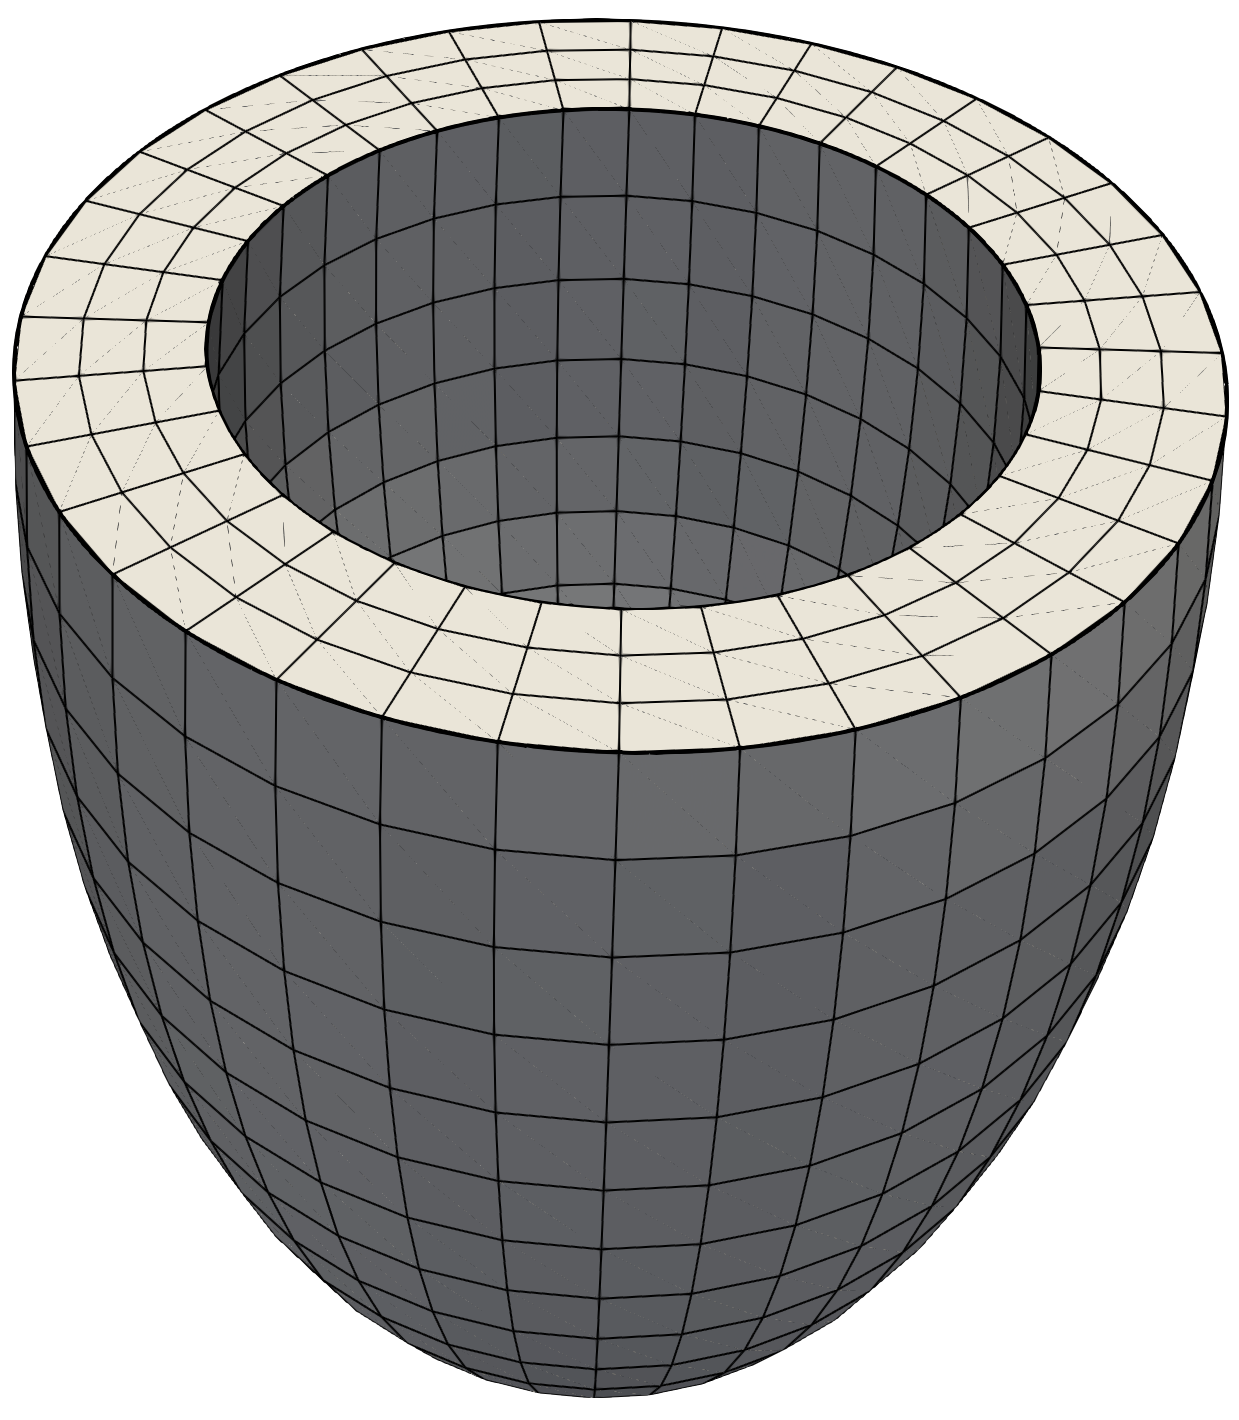
\includegraphics[width=0.4\textwidth]{figures/ventricle} 
	\subfigure[Ventricle undeformed geometry, showing the mesh with 1,620 cells]
	{
		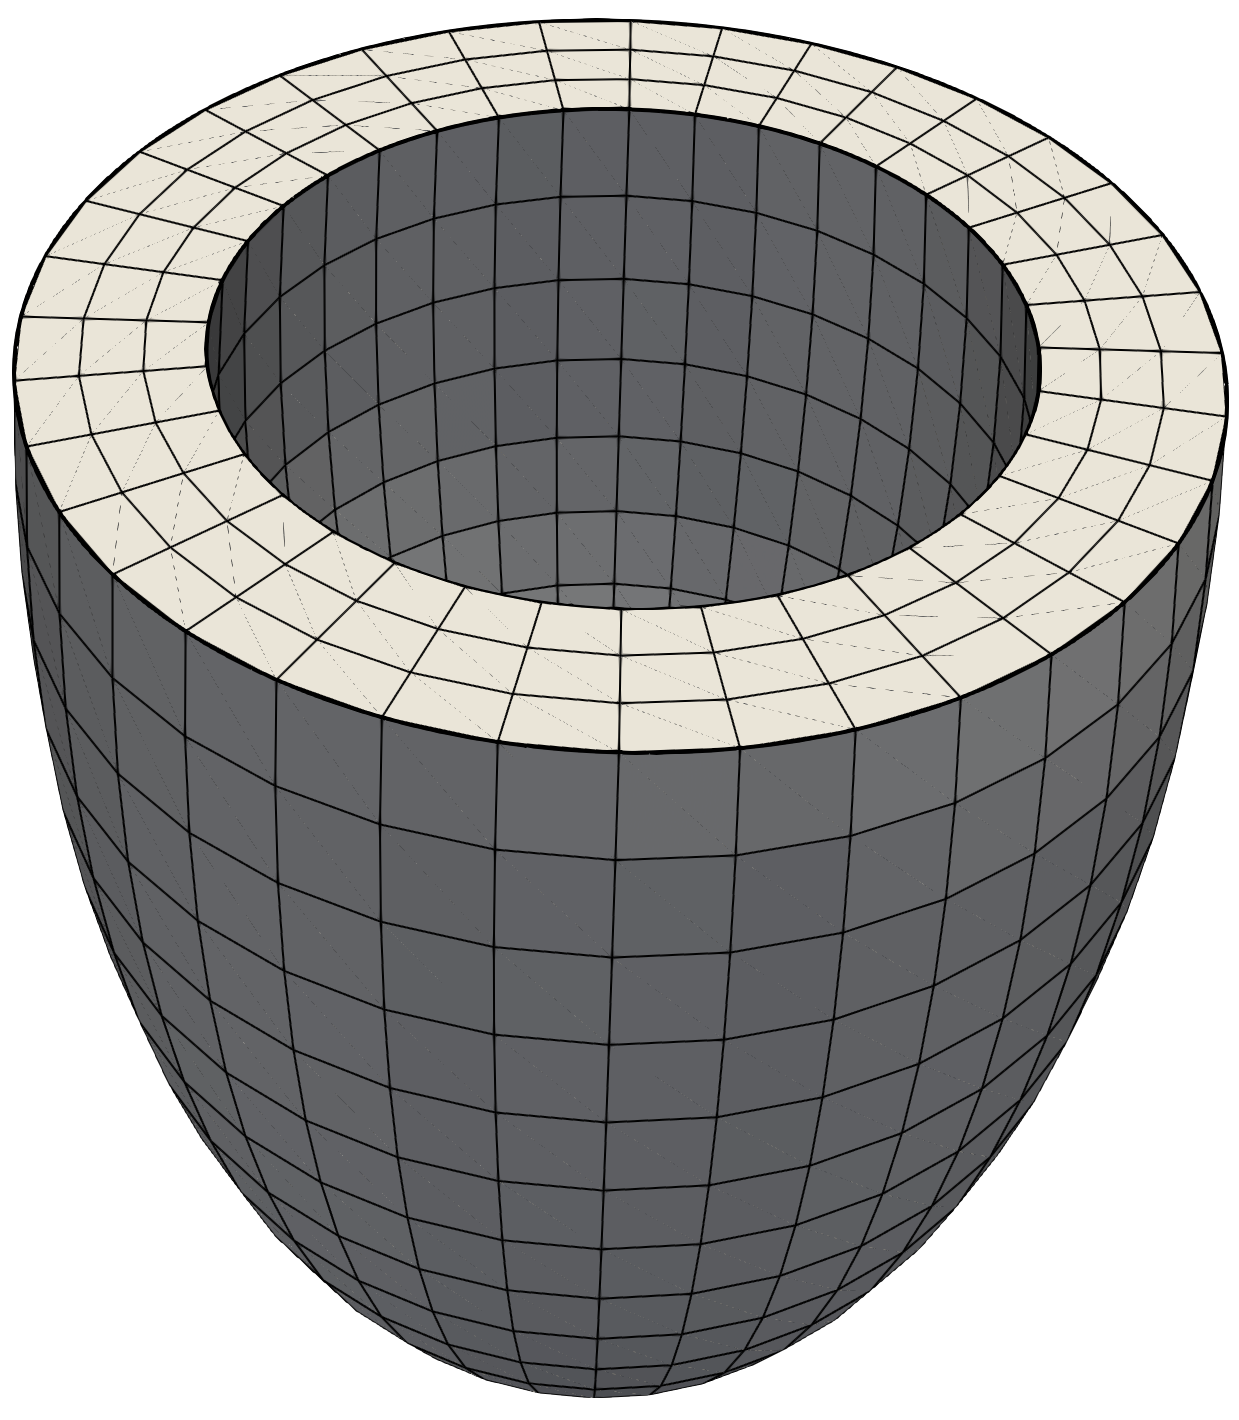
\includegraphics[height=0.46\textwidth]{figures/ventricle} 
	}
	\subfigure[Cross-section showing the equivalent (von Mises) stress distribution for the mesh with 829,440 cells]
	{
		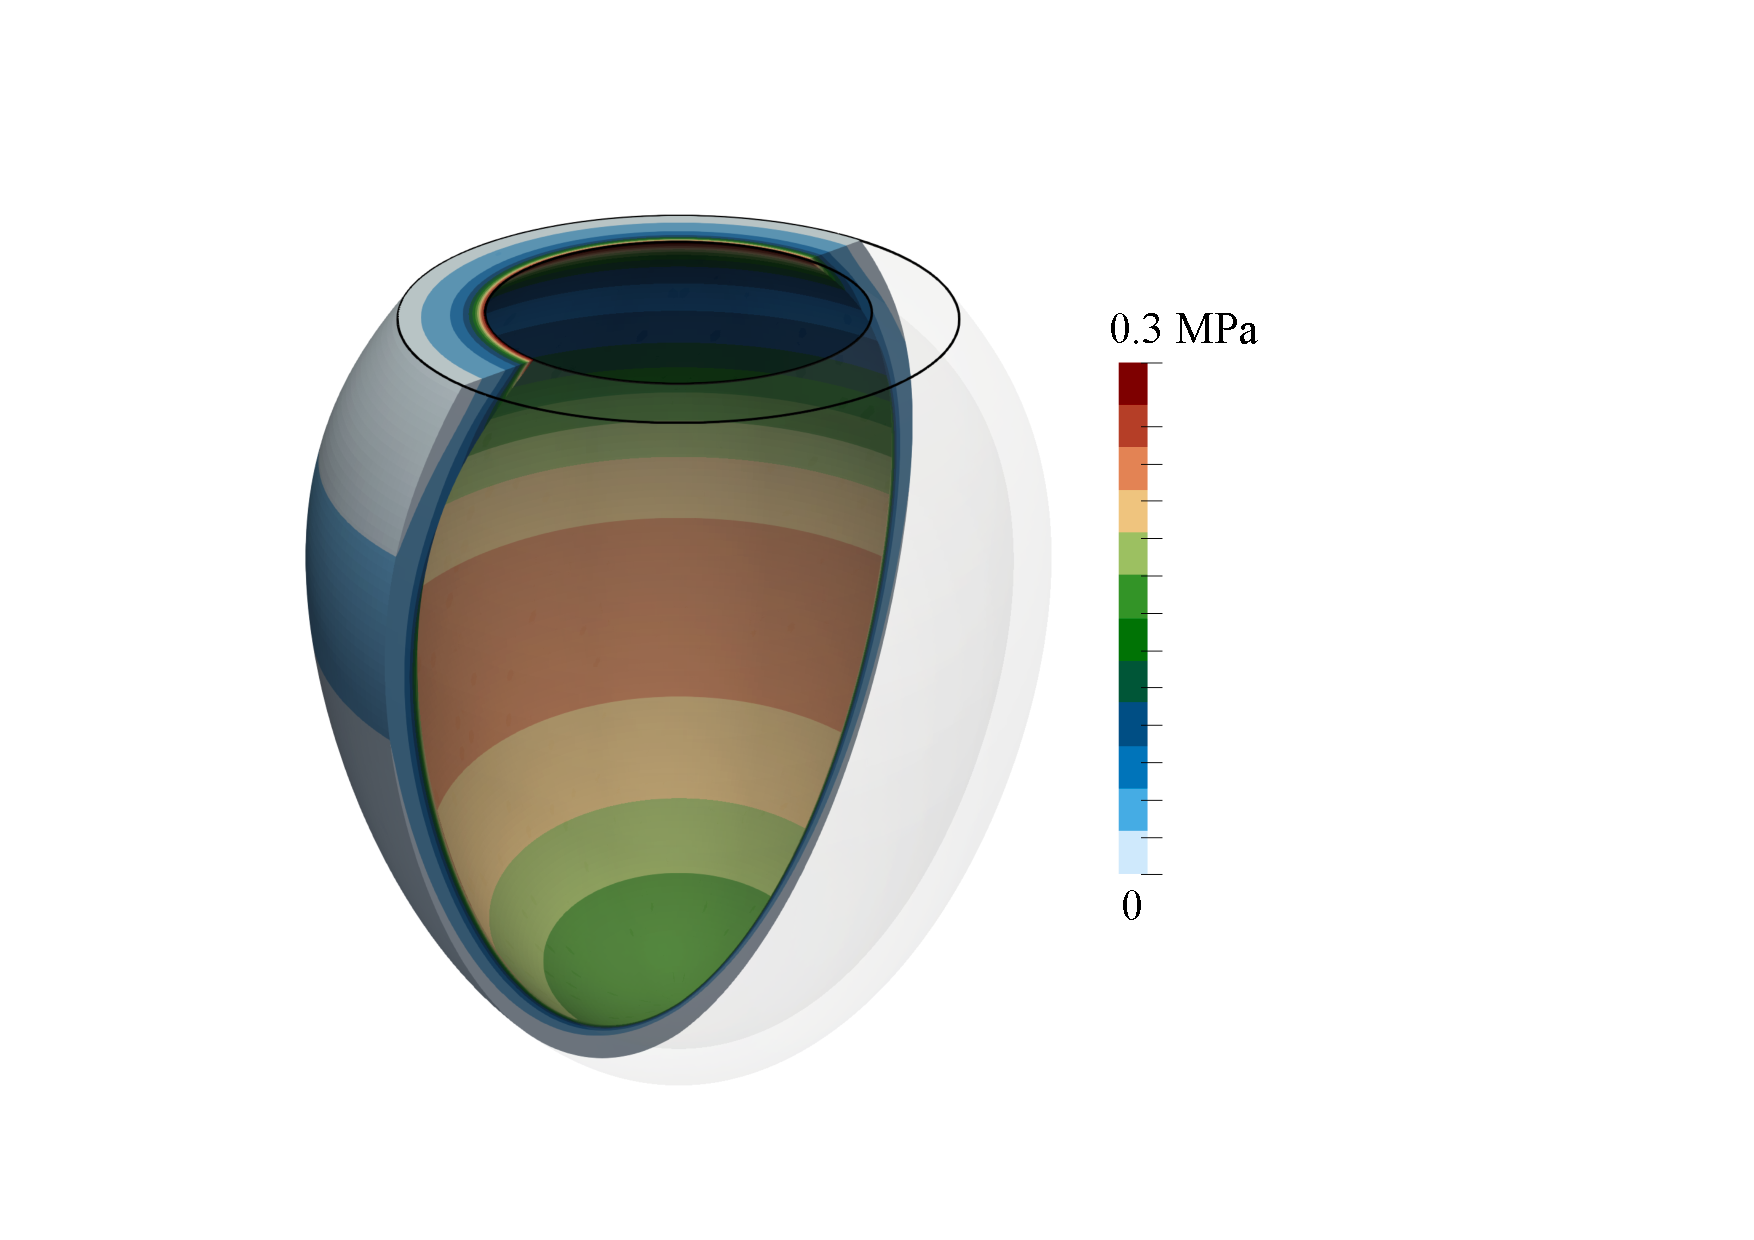
\includegraphics[height=0.48\textwidth]{figures/ventricle_sigmaEq}
	}
   \caption{Idealised ventricle case}
   \label{fig:ventricle}
\end{figure}

The equivalent (von Mises) stress at full inflation is shown for the mesh with 829,440 cells in Figure \ref{fig:ventricle}(b), where the high stresses on the endocardial (inner) surface quickly drop off through the wall thickness towards the endocardial (outer) surface.
The predicted deformed configuration of the midline of the ventricle wall is shown in Figure \ref{fig:ventricle_accuracy}, where a side-by-side comparison is given with the round-robin benchmark results from \citet{Land2015}.
The predictions are seen to become quickly mesh-independent and fall within the benchmark ranges.
%The variation in the round-robin results may be explained by the sensitivity of the predictions to the allowed compressibility; when a penalty bulk modulus approach is adopted, like in the current work, increasing
\begin{figure}[htbp]
	\centering
   		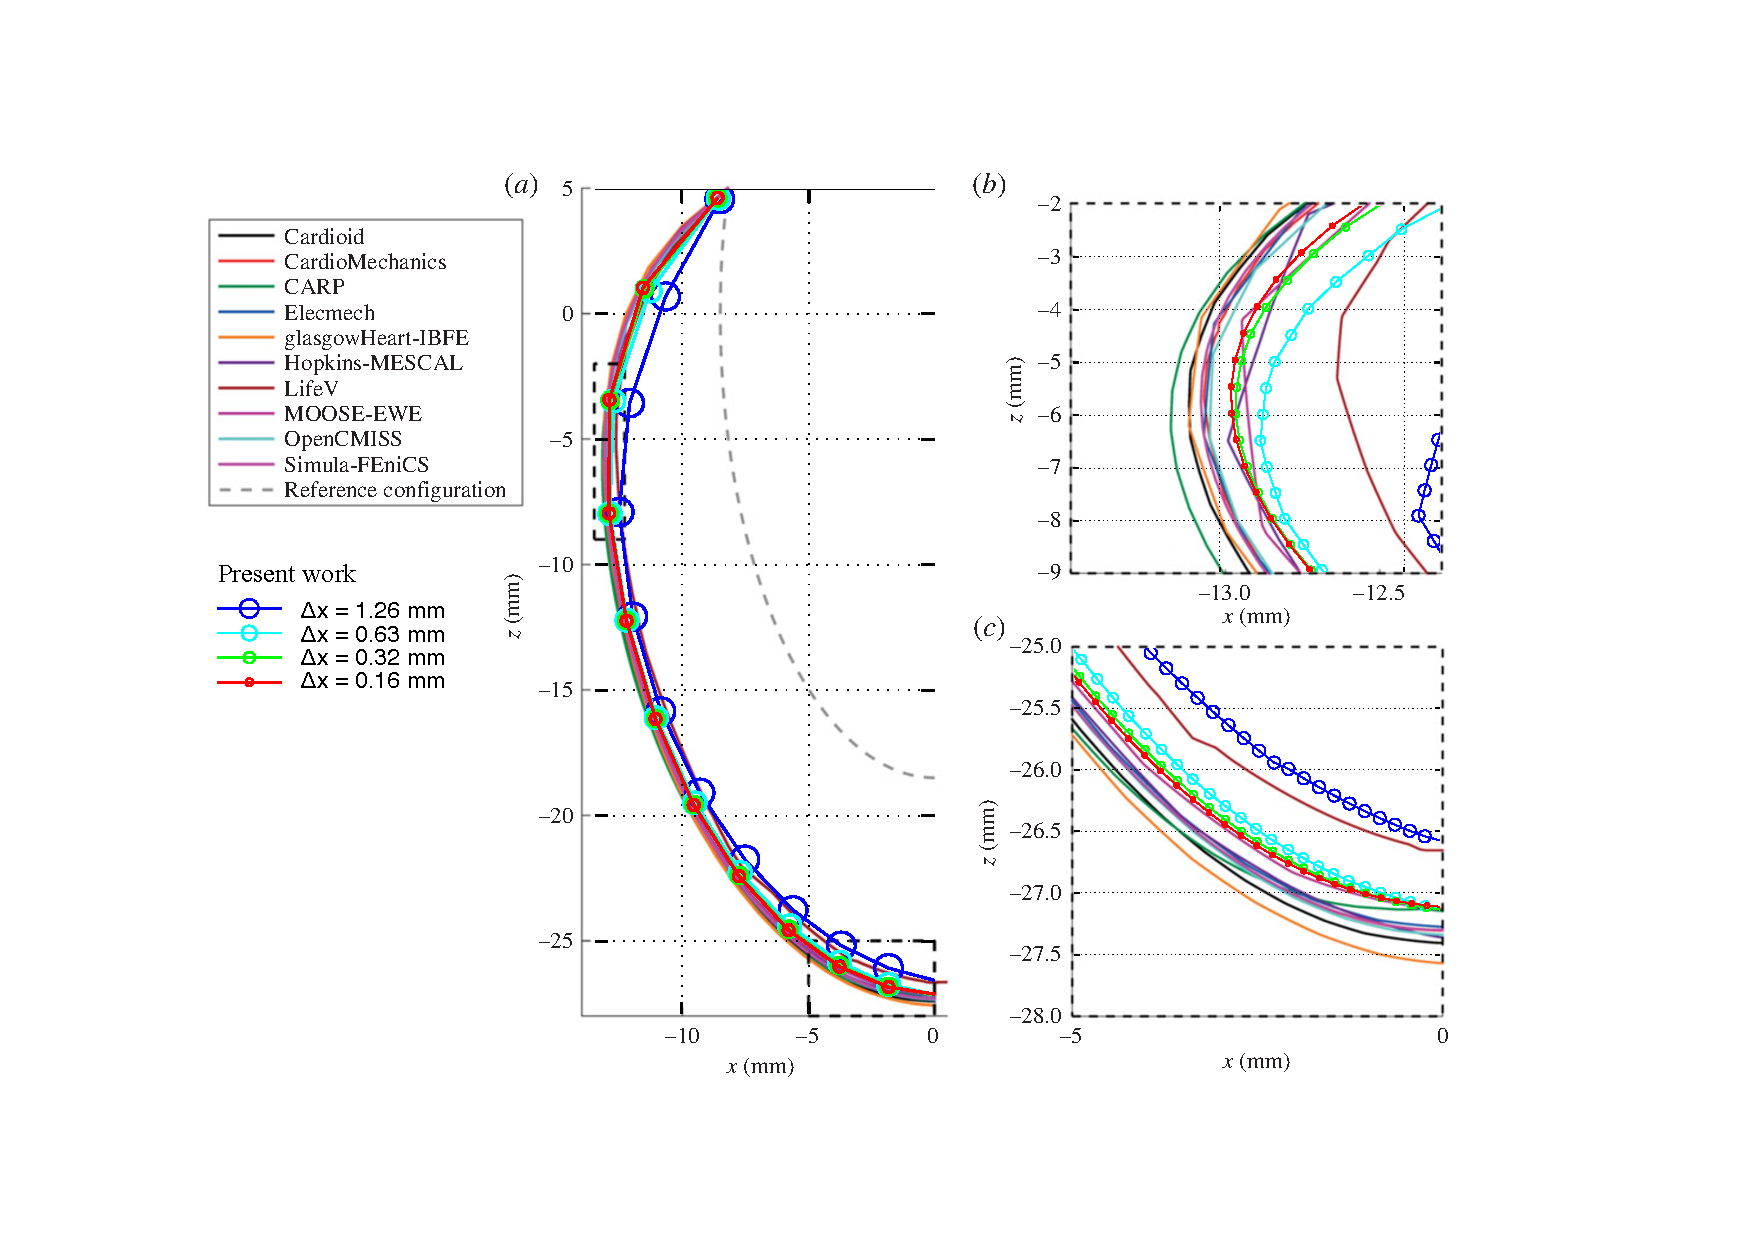
\includegraphics[width=0.6\textwidth]{figures/ventricle_results} 
%	\subfigure[Predictions from the current work]
%	{
%   		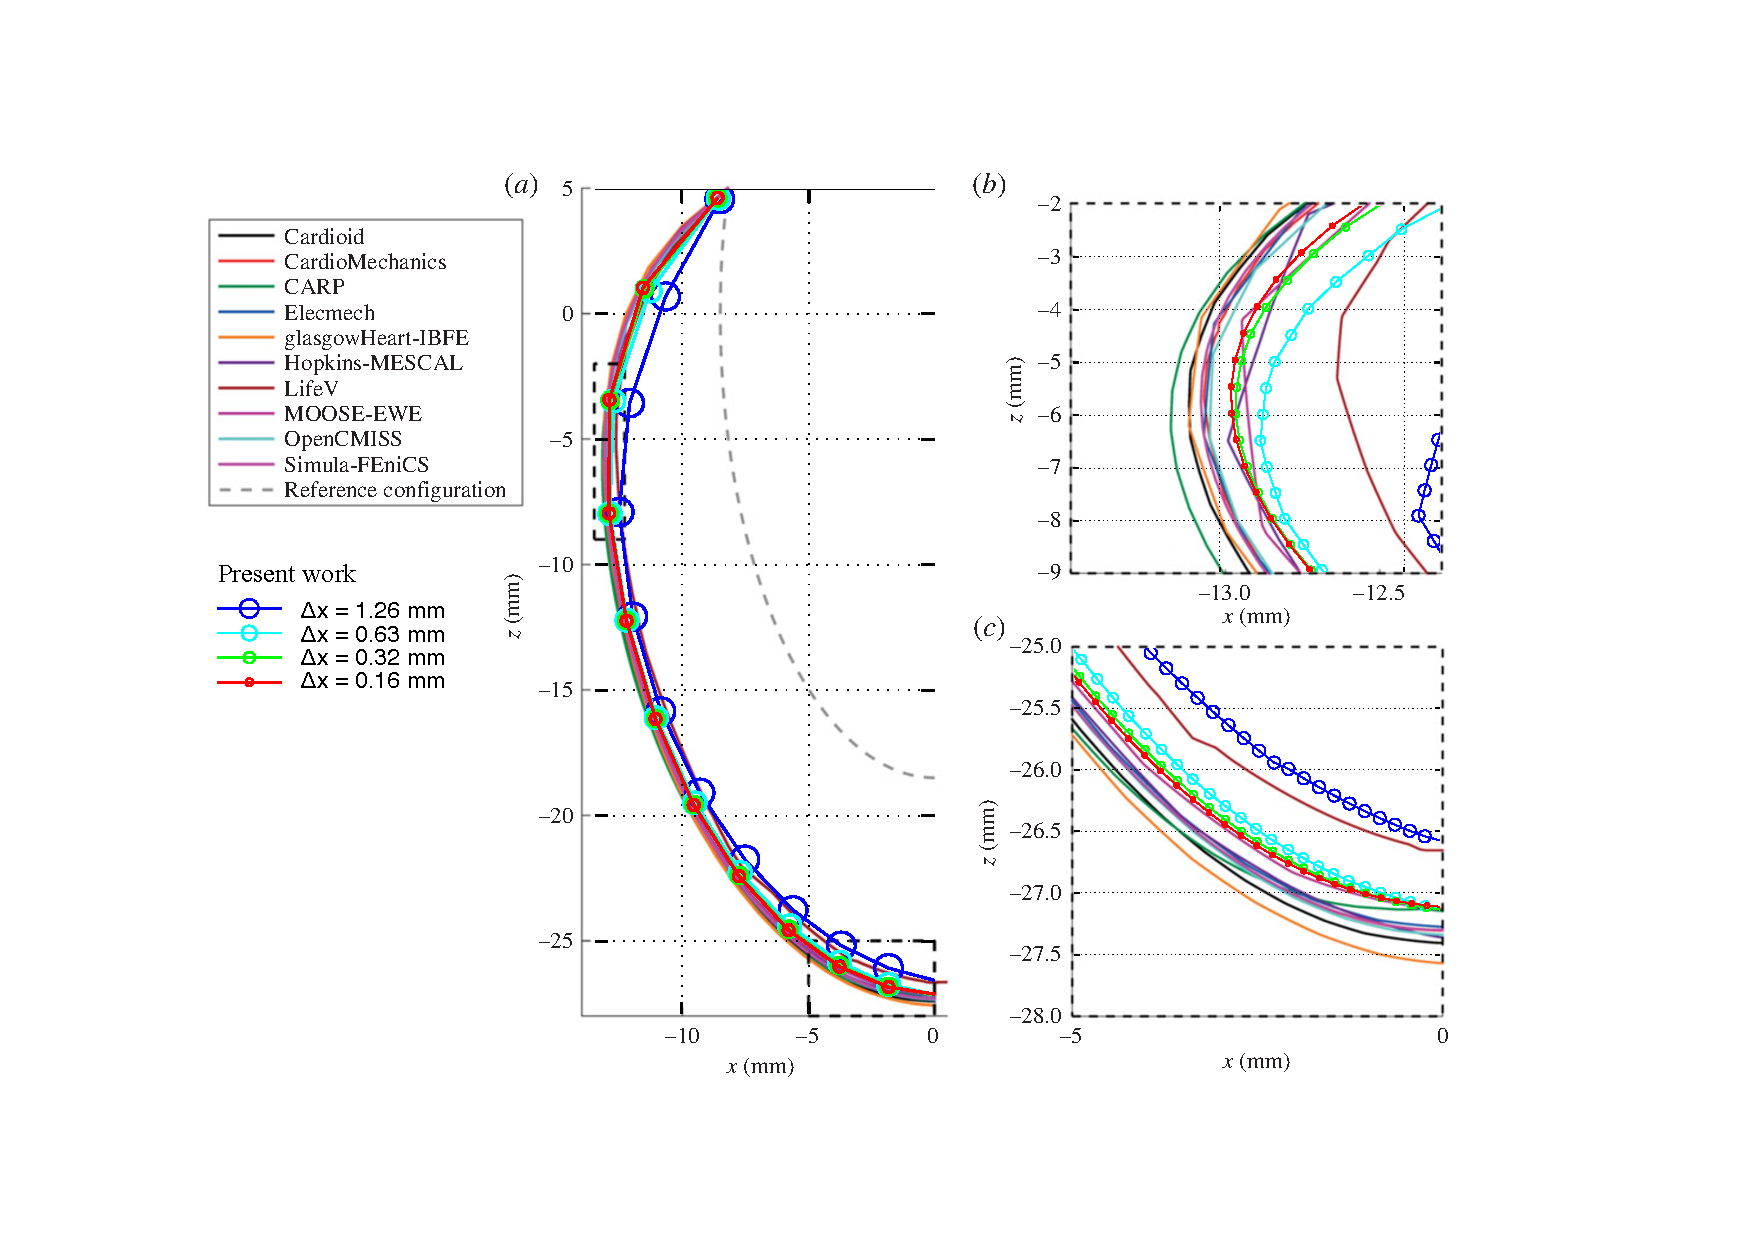
\includegraphics[width=0.46\textwidth]{figures/ventricle_results} 
%   	}
%	\subfigure[\citet{Land2015} benchmarks]
%	{
%		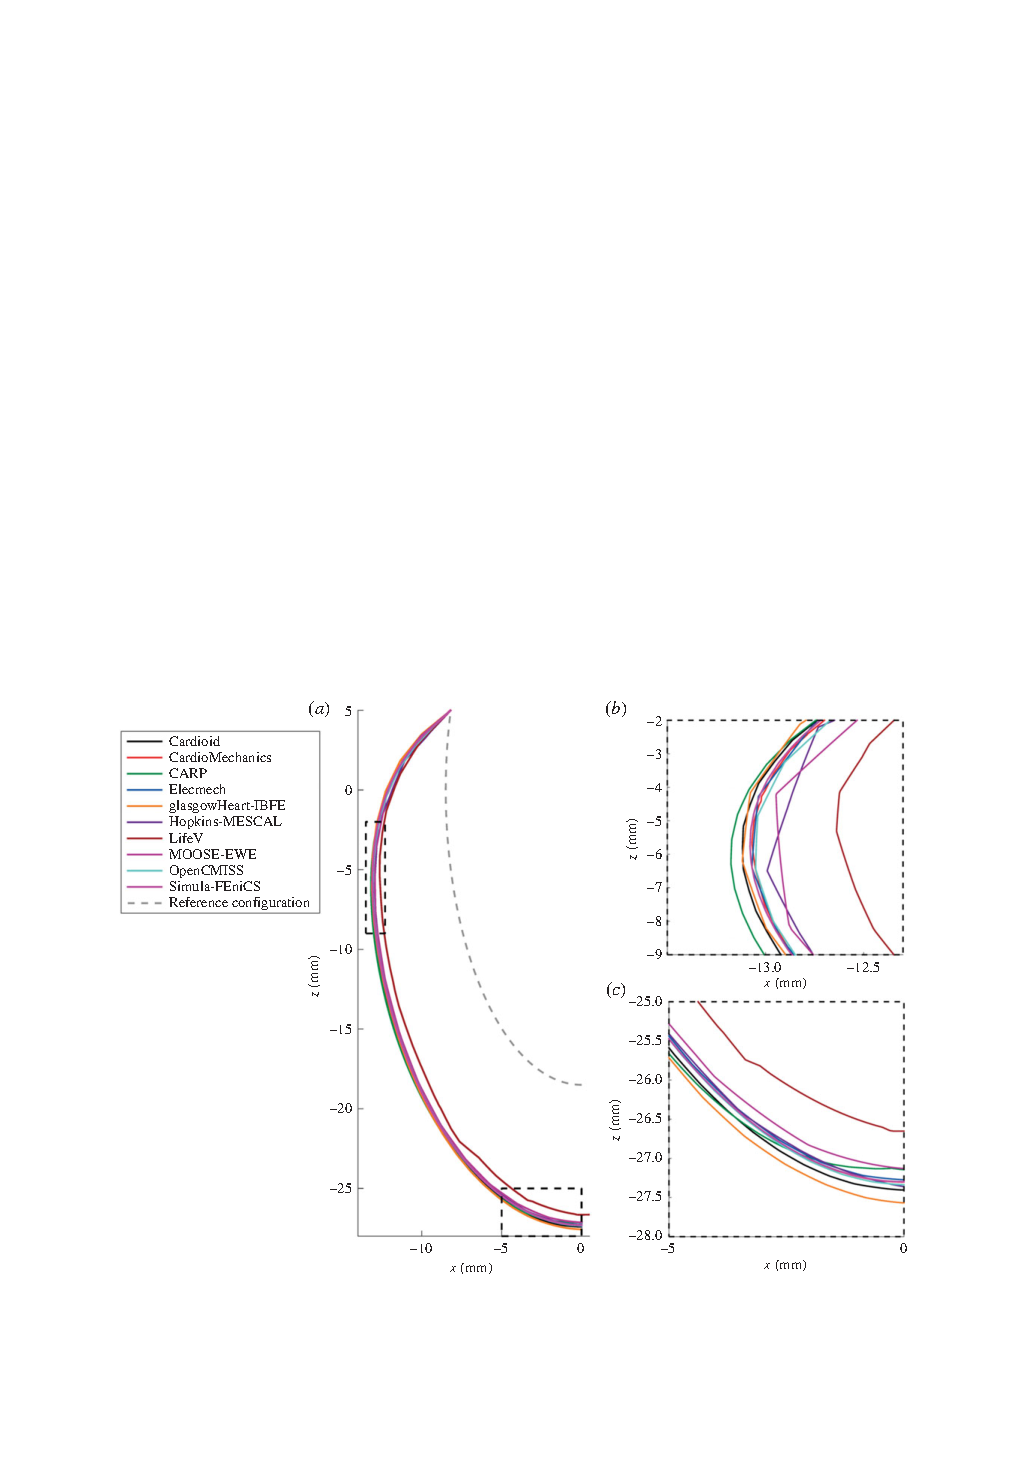
\includegraphics[width=0.48\textwidth]{figures/ventricle_results_land2015}  
%	}
	\caption{Idealised ventricle: predictions for the four meshes from the present work overlaid on the round-robin predictions from \citet{Land2015}}
	\label{fig:ventricle_accuracy}
\end{figure}


\paragraph{Case 5: Cook's membrane}
Cook's membrane (Figure \ref{fig:cooks_membrane}) is a well-known bending-dominated benchmark case used in linear and non-linear analysis.
The 2-D plane strain tapered panel (trapezoid) is fixed on one side and subjected to uniform shear traction on the opposite side.
The vertices of the trapezoid (in mm) are (0, 0), (48, 44), (48, 60),  and (0, 44).
The problem is solved quasi-statically, using 30 equally-sized loading increments, and there are no body forces.
%\begin{figure}[htbp]
%   \centering
%   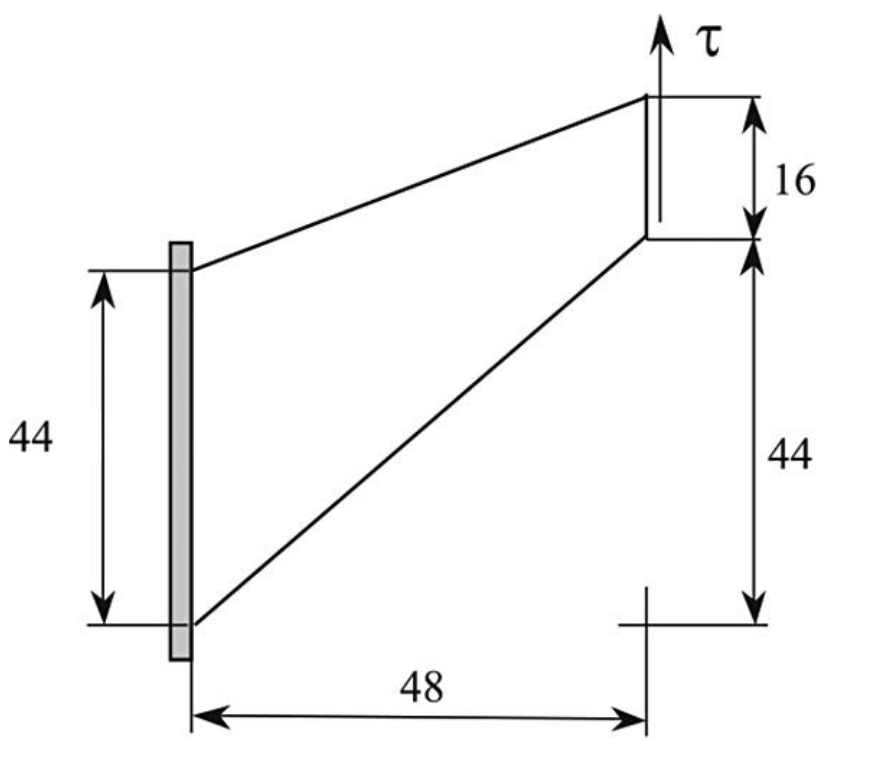
\includegraphics[width=0.4\textwidth]{figures/cooksMembrane-geometry} 
%   \caption{Cook's membrane case geometry (dimensions in mm) and loading conditions (fixed left, traction $\tau$ applied to right)}
%   \label{fig:cooks_membrane}
%\end{figure}
\begin{figure}[htbp]
	\centering
	\subfigure[Case geometry and dimensions]
	{
		\label{fig:cooks_membrane_geometry}
   		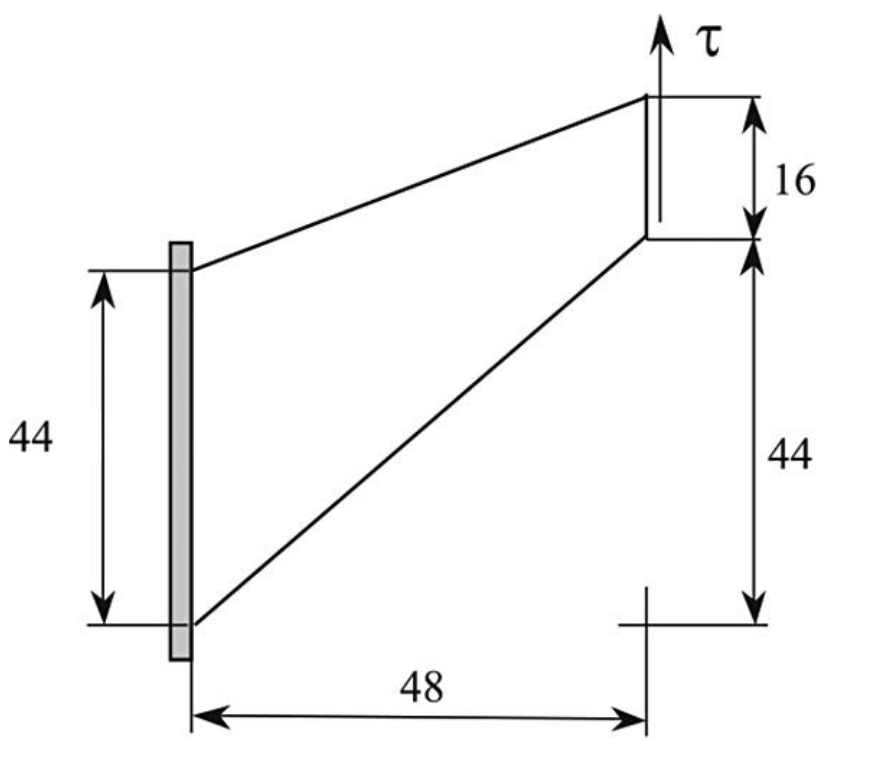
\includegraphics[scale=1]{figures/cooksMembrane-geometry} 
   	}
   	\qquad
	\subfigure[Hexahedral mesh with 144 cells]
	{
		\label{fig:cooks_membrane_mesh}
   		\includegraphics[scale=0.14]{figures/cooksMembrane-mesh}  
   	}
	\caption{Cook's membrane case geometry and mesh}
   \label{fig:cooks_membrane}
\end{figure}

The current work considers three forms of the problem:
\begin{enumerate}[label=\roman*.]
	\item Small strain linear elastic \cite{Zienkiewicz2000, Simplas}: $E=70$ MPa, $\nu=1/3$, and $\tau = 6250$ Pa.
	\item Finite strain neo-Hookean hyperelastic \cite{Pelteret2018}: $E=1.0985$ MPa, $\nu=0.3$, and $\tau = 0.0625$ MPa.
	\item Finite strain elastoplastic \citep{Simo1992, Simplas}: $E=206.9$ MPa, $\nu=0.29$, $\sigma_y = 0.45 + 0.12924\bar{\varepsilon}_p + (0.715 - 0.45)(1- e^{-16.93\bar{\varepsilon}_p})$ MPa, and $\tau = 0.3125$ MPa.
\end{enumerate}
where $E$ is the Young's modulus, $\nu$ is the Poisson's ratio, $\sigma_y$ is the yield strength, $\bar{\varepsilon}_p$ is the equivalent plastic strain, and $\tau$ is the prescribed shear traction.
%The Young's modulus $E = 206.9$ MPa and Poisson's ratio $\nu=0.29$, with the yield stress $\sigma_y$ given as \citep{Simo1992}
%\begin{eqnarray}
%	\sigma_y = \sigma_Y + H\bar{\varepsilon}_p + (\sigma_{\infty} - \sigma_Y)(1- e^{-\delta\bar{\varepsilon}_p})
%\end{eqnarray}
%The plastic yielding parameters are $\sigma_Y = 0.45$ MPa, $\sigma_{\infty} = 0.715$ MPa, $\delta = 16.93$, and $H = 0.12924$ MPa, where the hardening variable $\bar{\varepsilon}_p$ corresponds to equivalent plastic strain.
%\noindent
%\textbf{Sources for case i:} \cite{Zienkiewicz2000}\\
%O.C. Zienkiewicz, R.L. Taylor. The finite element method. Butterworth Heinemann, 2000.\\
%https://www.simplassoftware.com/benchmarks.html\#biblio-58\\
%https://github.com/spolanski/CoFEA/tree/master/benchmarks/02-cooks-membrane\\
%\textbf{Sources for case ii:} \cite{dealII95}\\
%https://www.dealii.org/current/doxygen/deal.II/code\_gallery\_Quasi\_static\_Finite\_strain\_Compressible\_Elasticity.html\\
%\textbf{Sources for case iii:} \citep{Simo1992}
Seven successively refined quadrilateral meshes are considered, where the cell counts are 9, 36, 144 (Figure \ref{fig:cooks_membrane}(b)), 576, $2\,304$, $9\,216$, and $36\,864$.
%mesh.1 - 3x3 - 9 CVs\\
%mesh.2 - 6x6 - 36 CVs\\
%mesh.3 - 12x12 - 144 CVs\\
%mesh.4 - 24x24 - 576 CVs\\
%mesh.5 - 48-48 - 2304 CVs\\
%mesh.6 - 96x96 - 9216 CVs\\
%mesh.7 - 192x192 - 36864 CVs

Figure \ref{fig:cooksMembrane_sigmaEq} shows the predicted equivalent stress distribution on the mesh with $36\,842$ cells for linear elastic, hyperelastic and hyperelastoplastic cases.
The stress distribution is consistent with bending, with regions of high stress near the upper and lower surfaces and a line of relatively unstressed material in the centre.
The greatest equivalent stresses occur at the top-left corner and the lower surface
In the hyperelastoplastic case, almost the entire domain is plastically yielding with only a small thin region remaining elastic, indicated by the blue line in Figure \ref{fig:cooksMembrane_sigmaEq}(c).
\begin{figure}[htbp]
   \centering
	\subfigure[Linear elastic case]
	{
		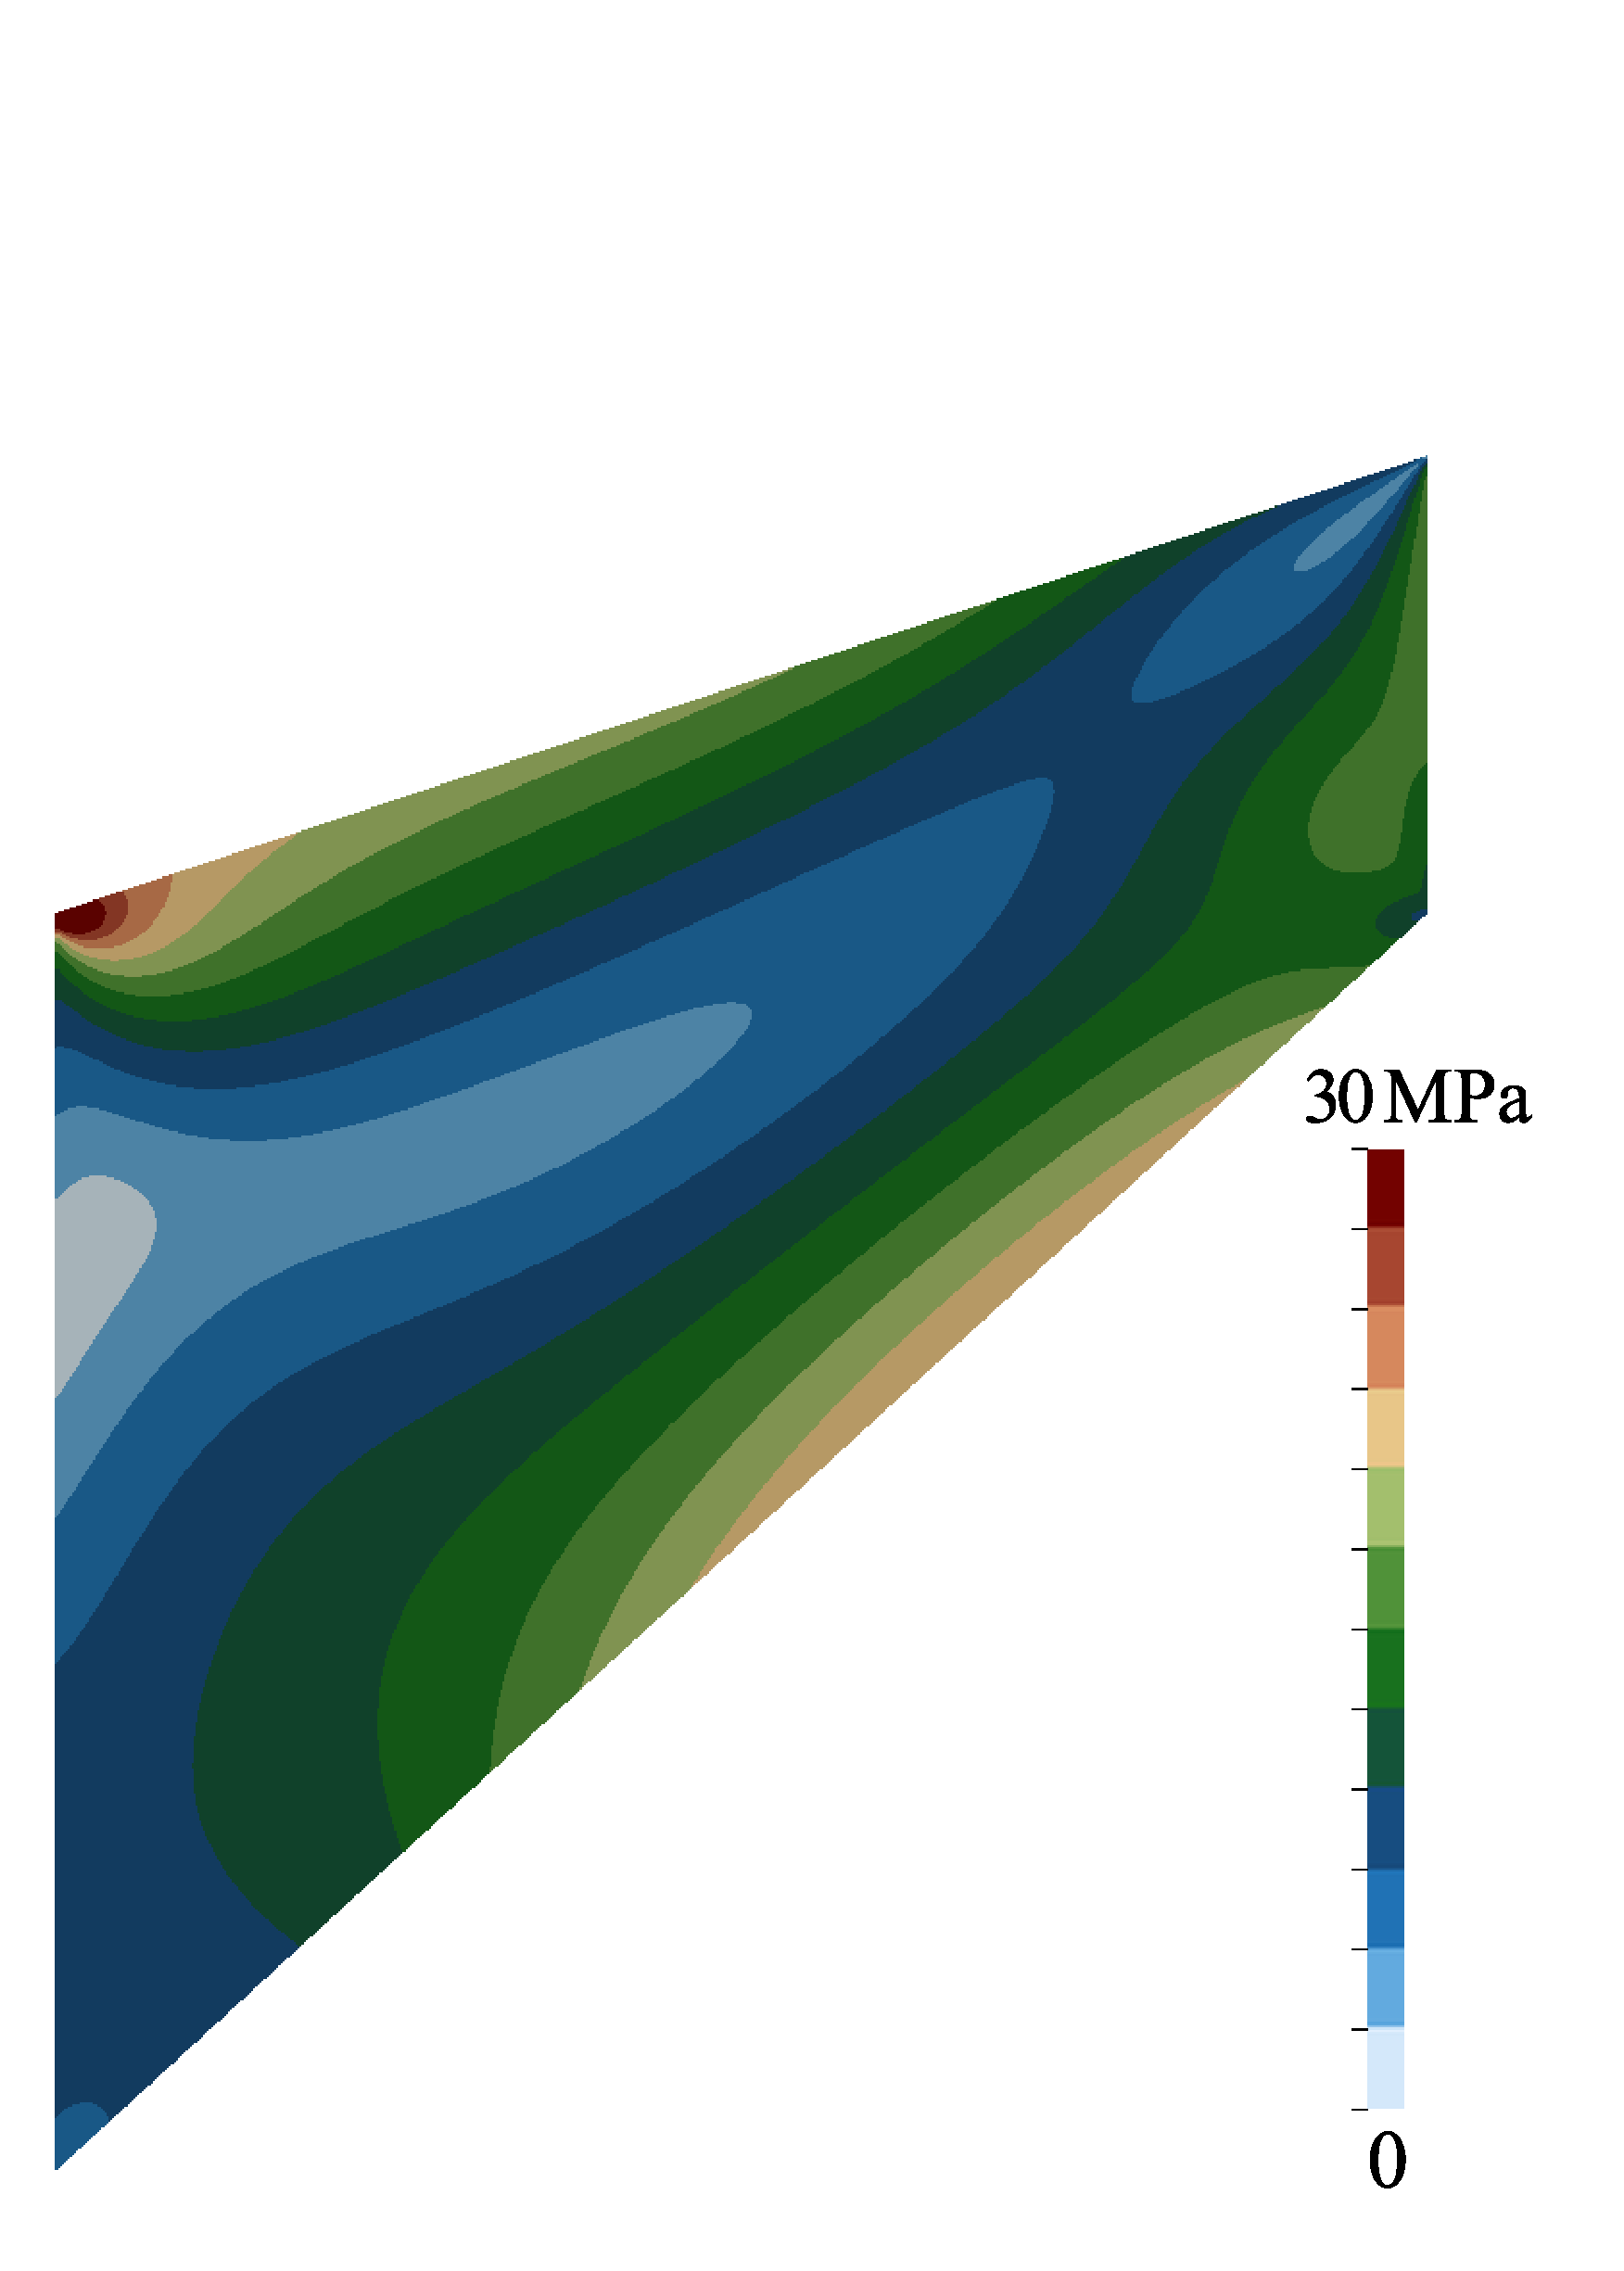
\includegraphics[width=0.3\textwidth]{figures/cooksMembrane-hookean-sigmaEq.pdf}  
	}
	\subfigure[Hyperelastic case]
	{
		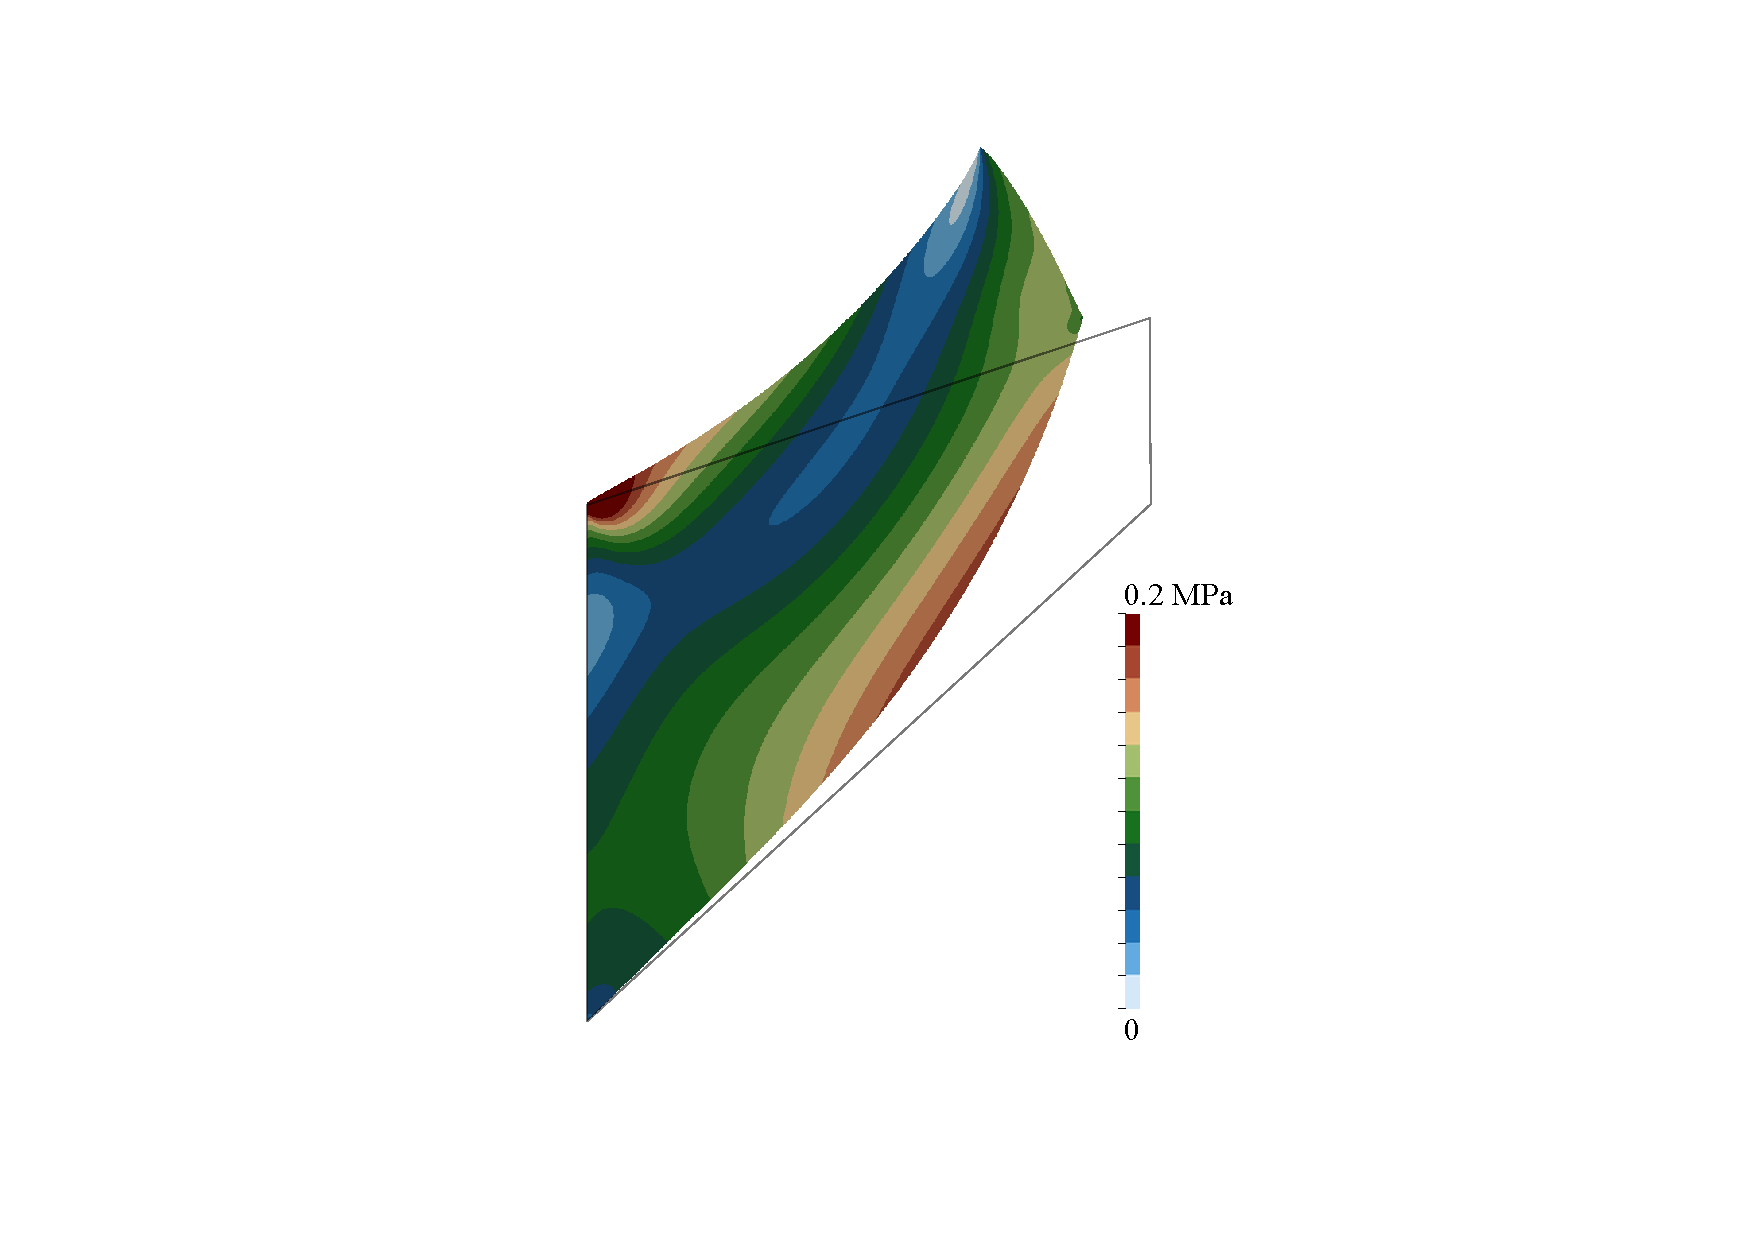
\includegraphics[width=0.3\textwidth]{figures/cooksMembrane-neoHookean-sigmaEq.pdf}  
	}
	\subfigure[Hyperelastoplastic case]
	{
		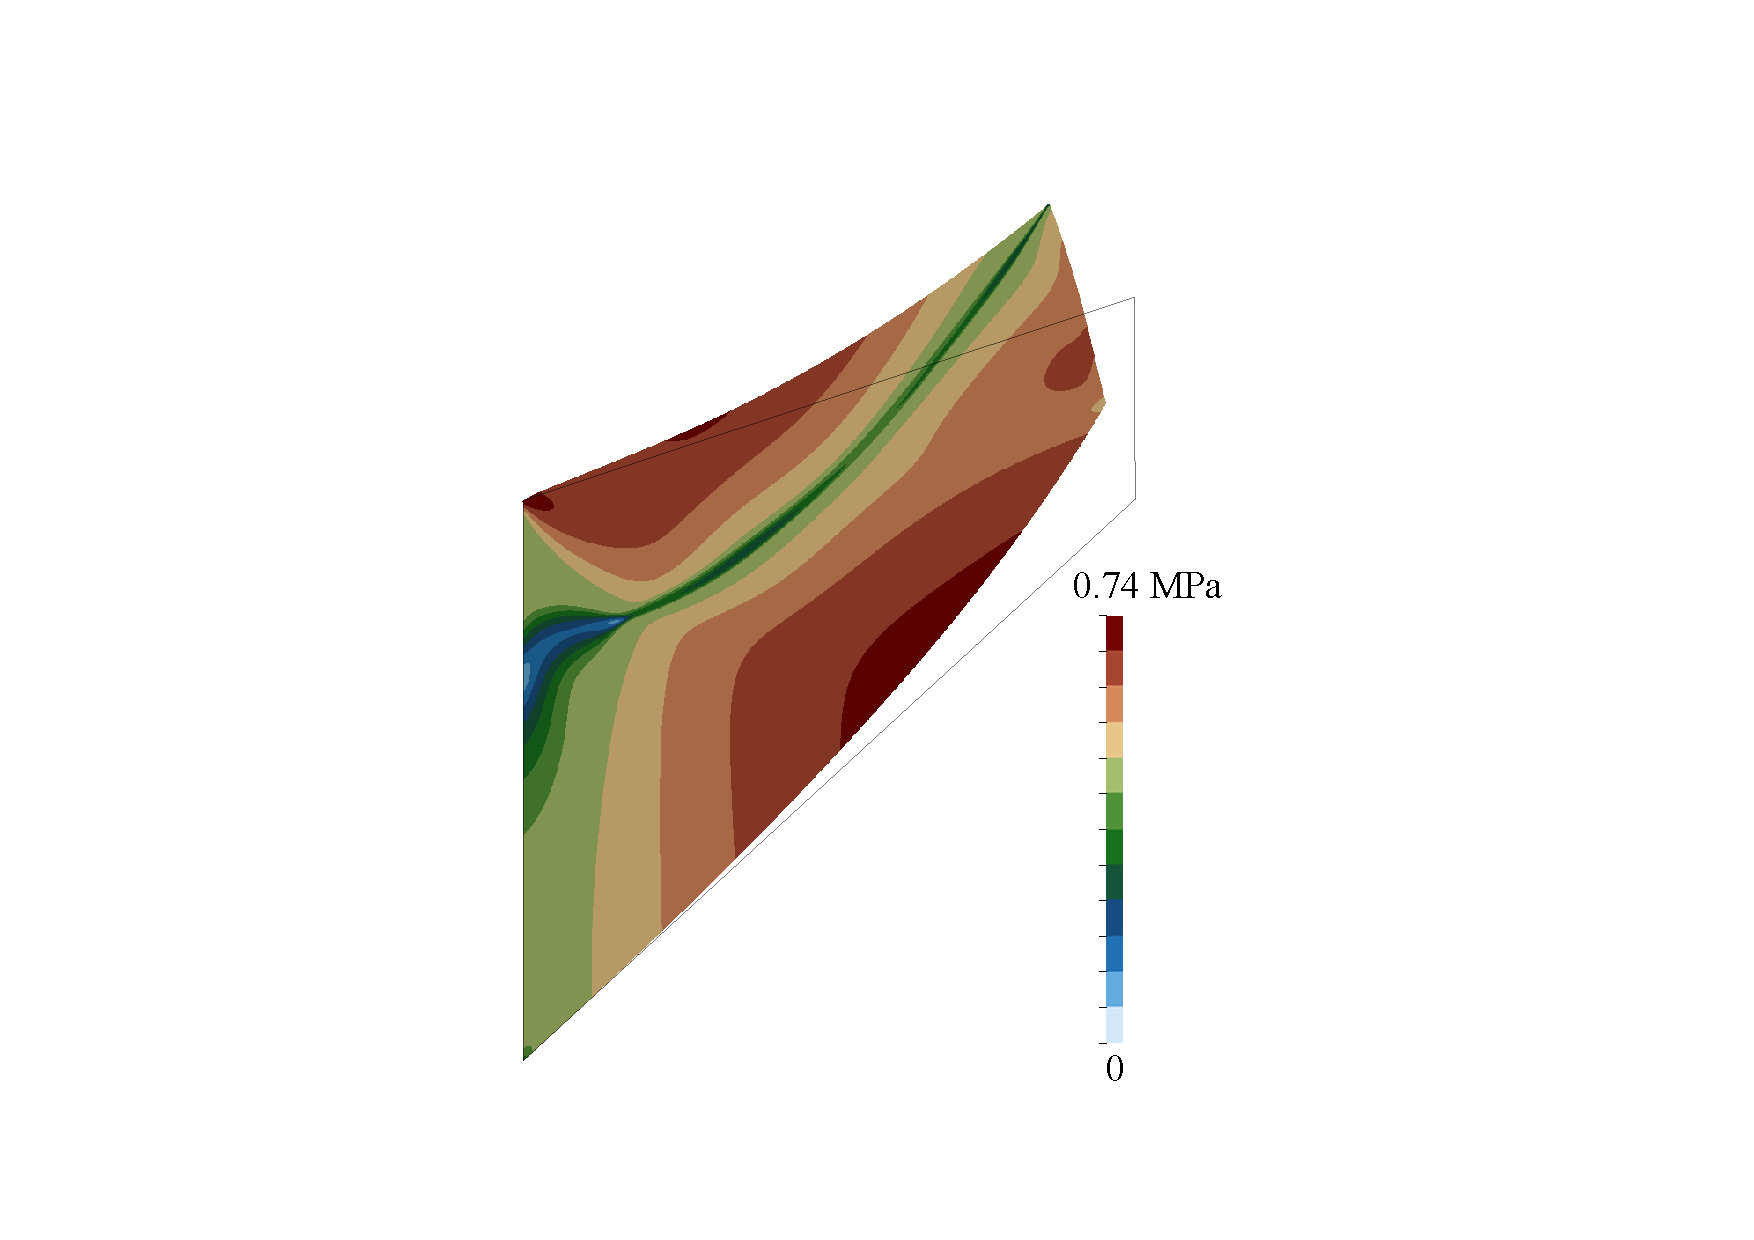
\includegraphics[width=0.3\textwidth]{figures/cooksMembrane-neoHookeanPlastic-sigmaEq.pdf}  
	}
   \caption{Equivalent (von Mises) stress distribution for the three Cook's membrane cases using the mesh with $36\,842$ cells}
   \label{fig:cooksMembrane_sigmaEq}
\end{figure}

Figure \ref{fig:cooksMembrane_disp} compares the predicted vertical displacement at the reference point as a function of the average cell widths with results from the literature.
The reference point is taken as the top right point -- (48,60) mm -- in the elastic and hyperelastoplastic cases, while it is taken as the midway point of the loading surface -- (48,52) mm -- in the hyperelastic case.
%\hl{Comment on results -> good/bad/etc}
%\hl{Comment on JFNK not working for plasticty}\\
%\hl{Philip, I'll leave this to you to comment on, as you'll be able to explain it better.}
\begin{figure}[htbp]
   \centering
   	\subfigure[Linear elastic case]
	{
		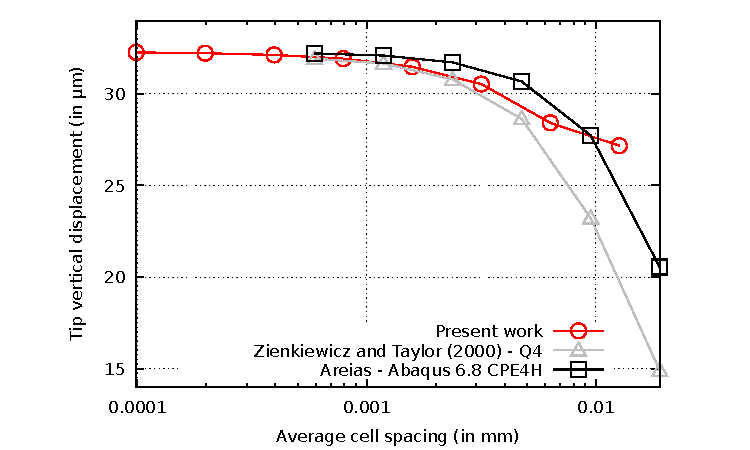
\includegraphics[width=0.45\textwidth]{figures/cooksMembrane-hookeanTipDispConvergence}  
	}
	\subfigure[Hyperelastic case]
	{
		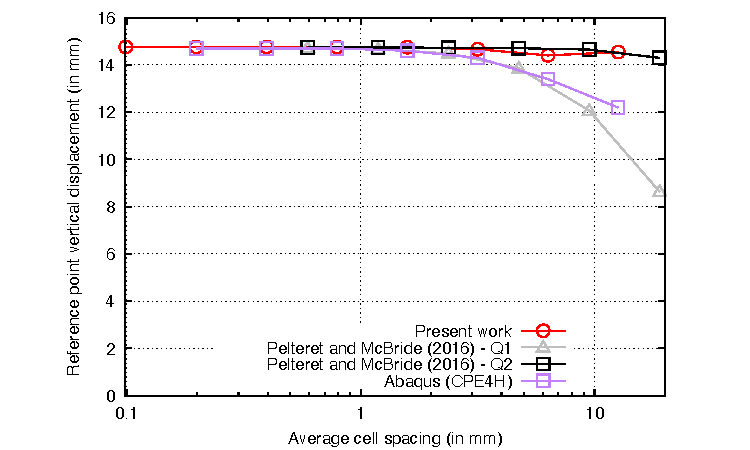
\includegraphics[width=0.45\textwidth]{figures/cooksMembrane-neoHookeanTipDispConvergence}  
	}
	\subfigure[Hyperelastoplastic case]
	{
		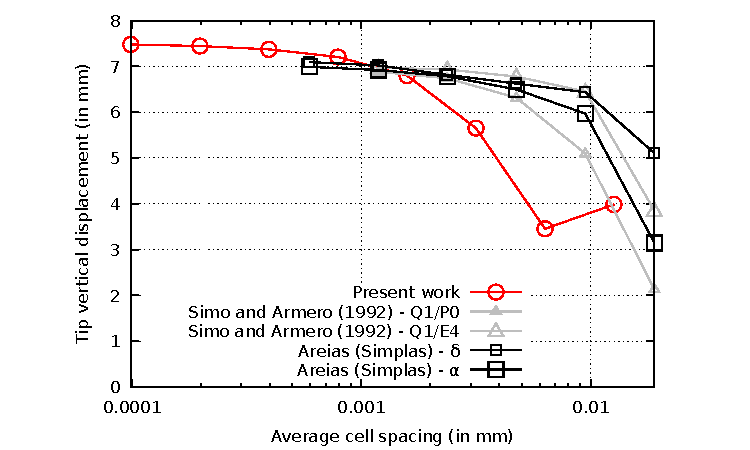
\includegraphics[width=0.45\textwidth]{figures/cooksMembrane-neoHookeanPlasticTipDispConvergence}  
	}
%	\subfigure[Equivalent stress distribution for the hyperelastic case (case ii) using the mesh with $36\,842$ cells]
%	{
%		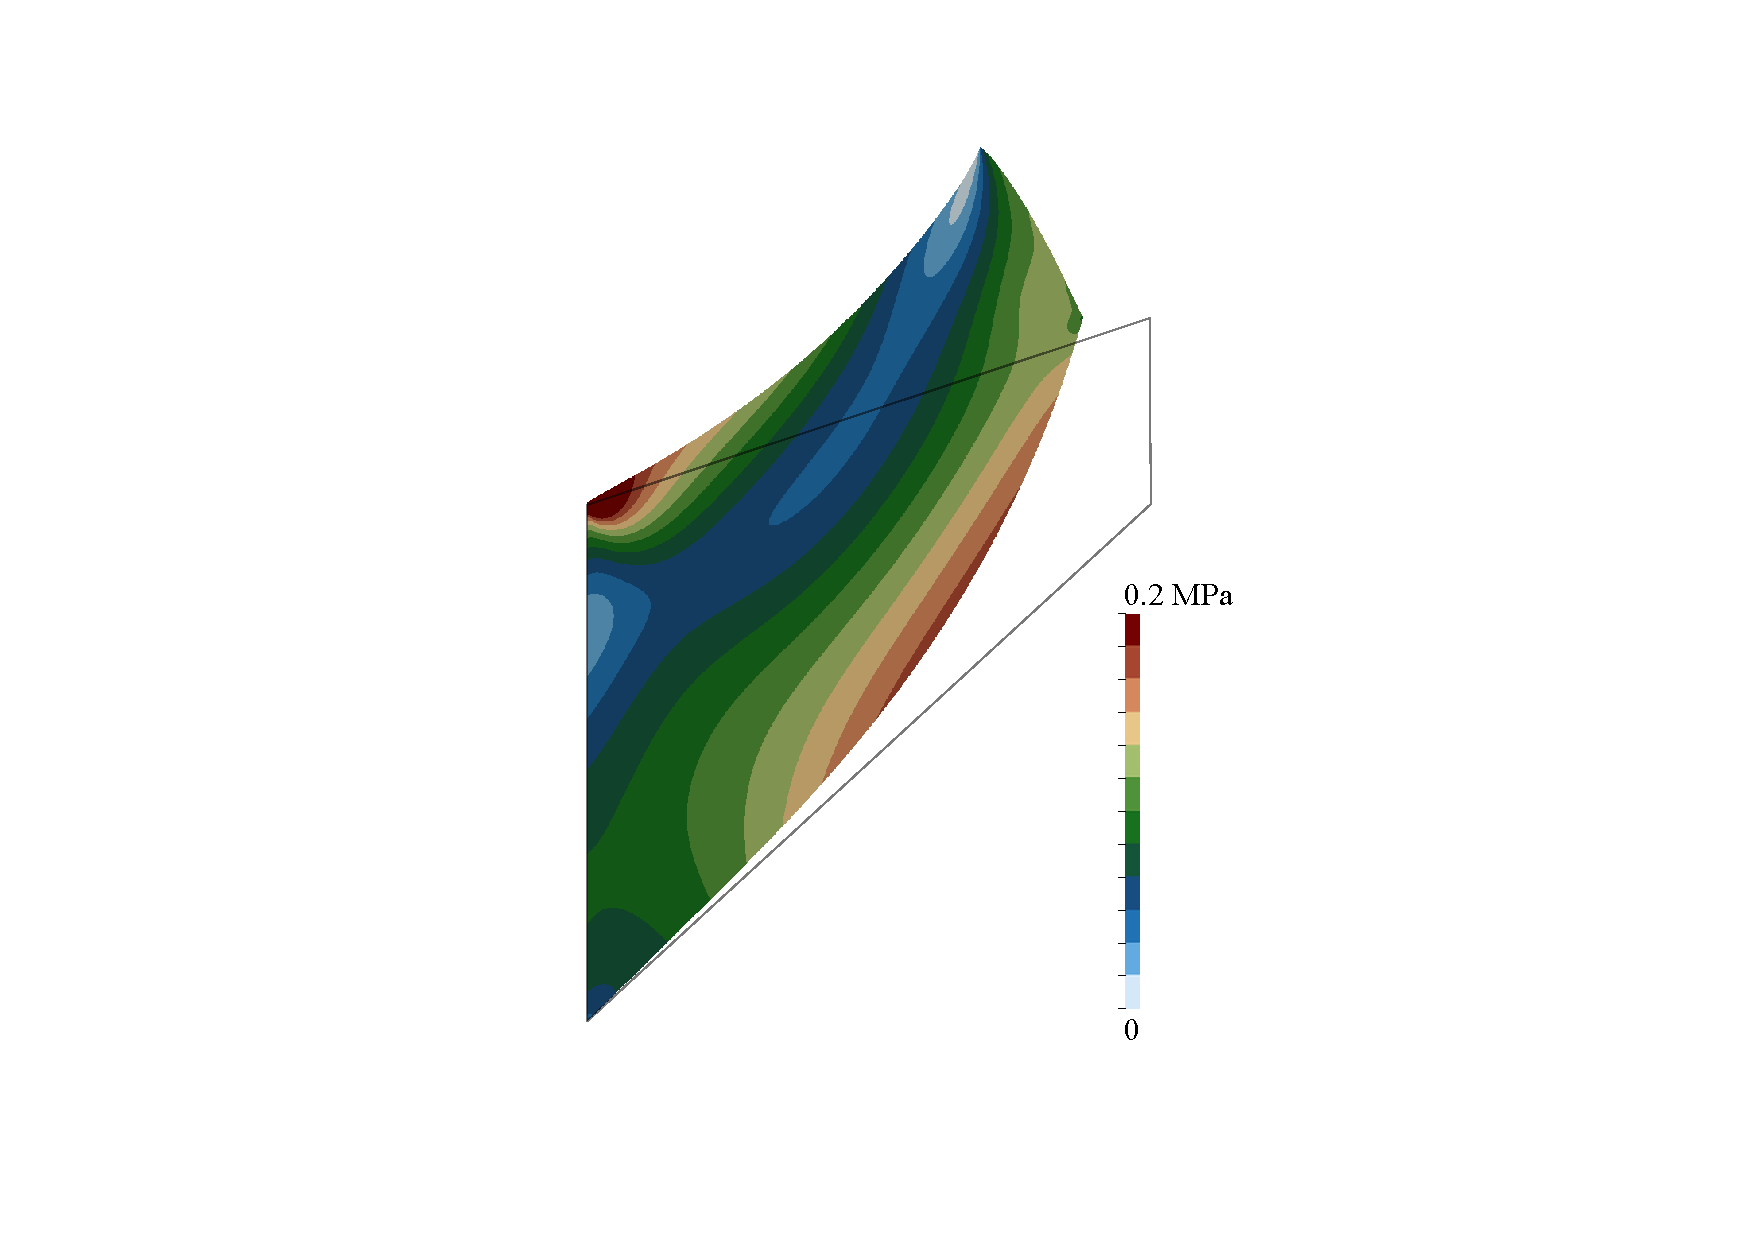
\includegraphics[height=0.5\textwidth]{figures/cooksMembrane-sigmaEq.pdf}  
%	}
%	\subfigure[Convergence of tip (48,60) vertical displacement, normalised using the displacement value from the finest mesh (given in parentheses)]
%	{
%		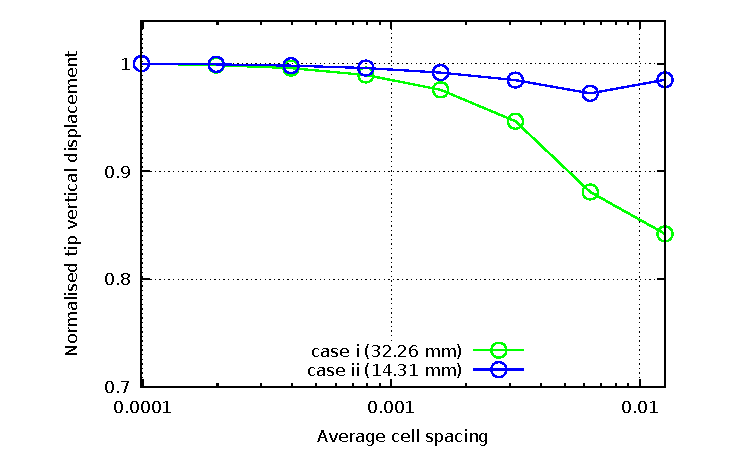
\includegraphics[height=0.35\textwidth]{figures/cooksMembrane-tipDispConvergence.pdf} 
%	}
   \caption{Cook's membrane vertical displacement predictions at the reference point as a function of the average cell width. Comparisons are given with the results from \cite{Zienkiewicz2000, Pelteret2018, Simo1992, Simplas}.}
   \label{fig:cooksMembrane_disp}
\end{figure}

No difference is seen in the predictions whether using the Jacobian-free Newton-Krylov or segregated approach, assuming convergence is achieved.
This is expected since both use the same discretisation, and the solution tolerances are shown to ensure the iteration errors are small.
Consequently, only the Jacobian-free Newton-Krylov results are shown for the linear elastic and hyperelastic cases.
However, the Jacobian-free Newton-Krylov showed poor convergence in the hyperelastoplastic case and failed to converge on many of the meshes.
As a result, the results for the segregated approach are presented instead for the hyperelastoplastic case.
Discussion of the relative convergence and robustness of the Jacobian-free Newton-Krylov and segregated methods is left to Section \ref{sec:resource_requirements}.
%I ran the hyperelastic case with the TLTD solver and the hyperelastoplastic case with the UL solver. This combination produced the "nicest" convergence curves}



\paragraph{Case 6: Vibration of a 3-D Cantilevered Beam}
This 3-D, dynamic, finite strain case geometry consists of a $2 \times 0.2 \times 0.2$ m cuboid column and was proposed in its initial form by \citet{Tukovic2007}.
%(Figure \ref{fig:dynamic_cantilever})
%A sudden, constant traction $\bb{T} = \left(\sfrac{|\bb{T}|}{\sqrt{2}}\right) \left(1, 1, 0 \right)$ Pa is applied to the upper surface, where the magnitude $|\bb{T}|$ is defined in terms of a dimensionless load factor $\mathcal{F}$ as
%\begin{eqnarray}
%	|\bb{T}| = \frac{\mathcal{F} E I}{A L^2} \text{ Pa}
%\end{eqnarray}
A sudden, constant traction $\bb{T} = \left(0.1, 0.1, 0 \right)$ MPa is applied to the upper surface.
%A sudden, constant traction $\bb{T} = \left(\sfrac{|\bb{T}|}{\sqrt{2}}\right) \left(1, 1, 0 \right)$ Pa is applied to the upper surface, where the magnitude $|\bb{T}|$ is defined in terms of a dimensionless load factor $\mathcal{F}$ as
%In the current study, $\mathcal{F} = 1$.
A neo-Hookean hyperelastic material is assumed with $E = 15.293$ MPa, $\nu = 0.3$ and density $\rho = 1000$ kg m$^{-3}$, while the area $A = 0.04$ m$^2$ and the second moment of area $I = \frac{1}{7\,500}$ m$^4$. %0.0001333
The geometric and material parameters were chosen for the first natural frequency to be 1 Hz in the small strain limit.
The magnitude of the applied traction was chosen to ensure significant geometric nonlinearity, with the upper surface of the beam expected to drop below the plane of the lower surface.
Four succesively refined hexahedral meshes are generated using the OpenFOAM \texttt{blockMesh} utility, with cell counts of 270, $2\,160$, $17\,280$ and $138\,240$.
%A fixed time step size of 0.001617274174 s is chosen, corresponding to a Courant number of six on the mesh with $2\,160$ cells.
%A fixed time step size of 1 ms is chosen.
The time step size is 1 ms, and the total period is 10 s.
% corresponding to 10 expected oscillation periods.
%, corresponding to a Courant number of six on the mesh with $2\,160$ cells.

The deformed configuration of the beam at six time steps is shown in Figure \ref{fig:dynamic_cantilever}(a) for the mesh with $2\,160$ cells, where the upper surface is seen to drop below the horizontal from approximately t = 0.2 s to 0.32 s.
The corresponding displacement magnitude of the centre of the upper surface of the beam vs time is shown in Figure \ref{fig:dynamic_cantilever}(b).
\begin{figure}[htbp]
   \centering
%   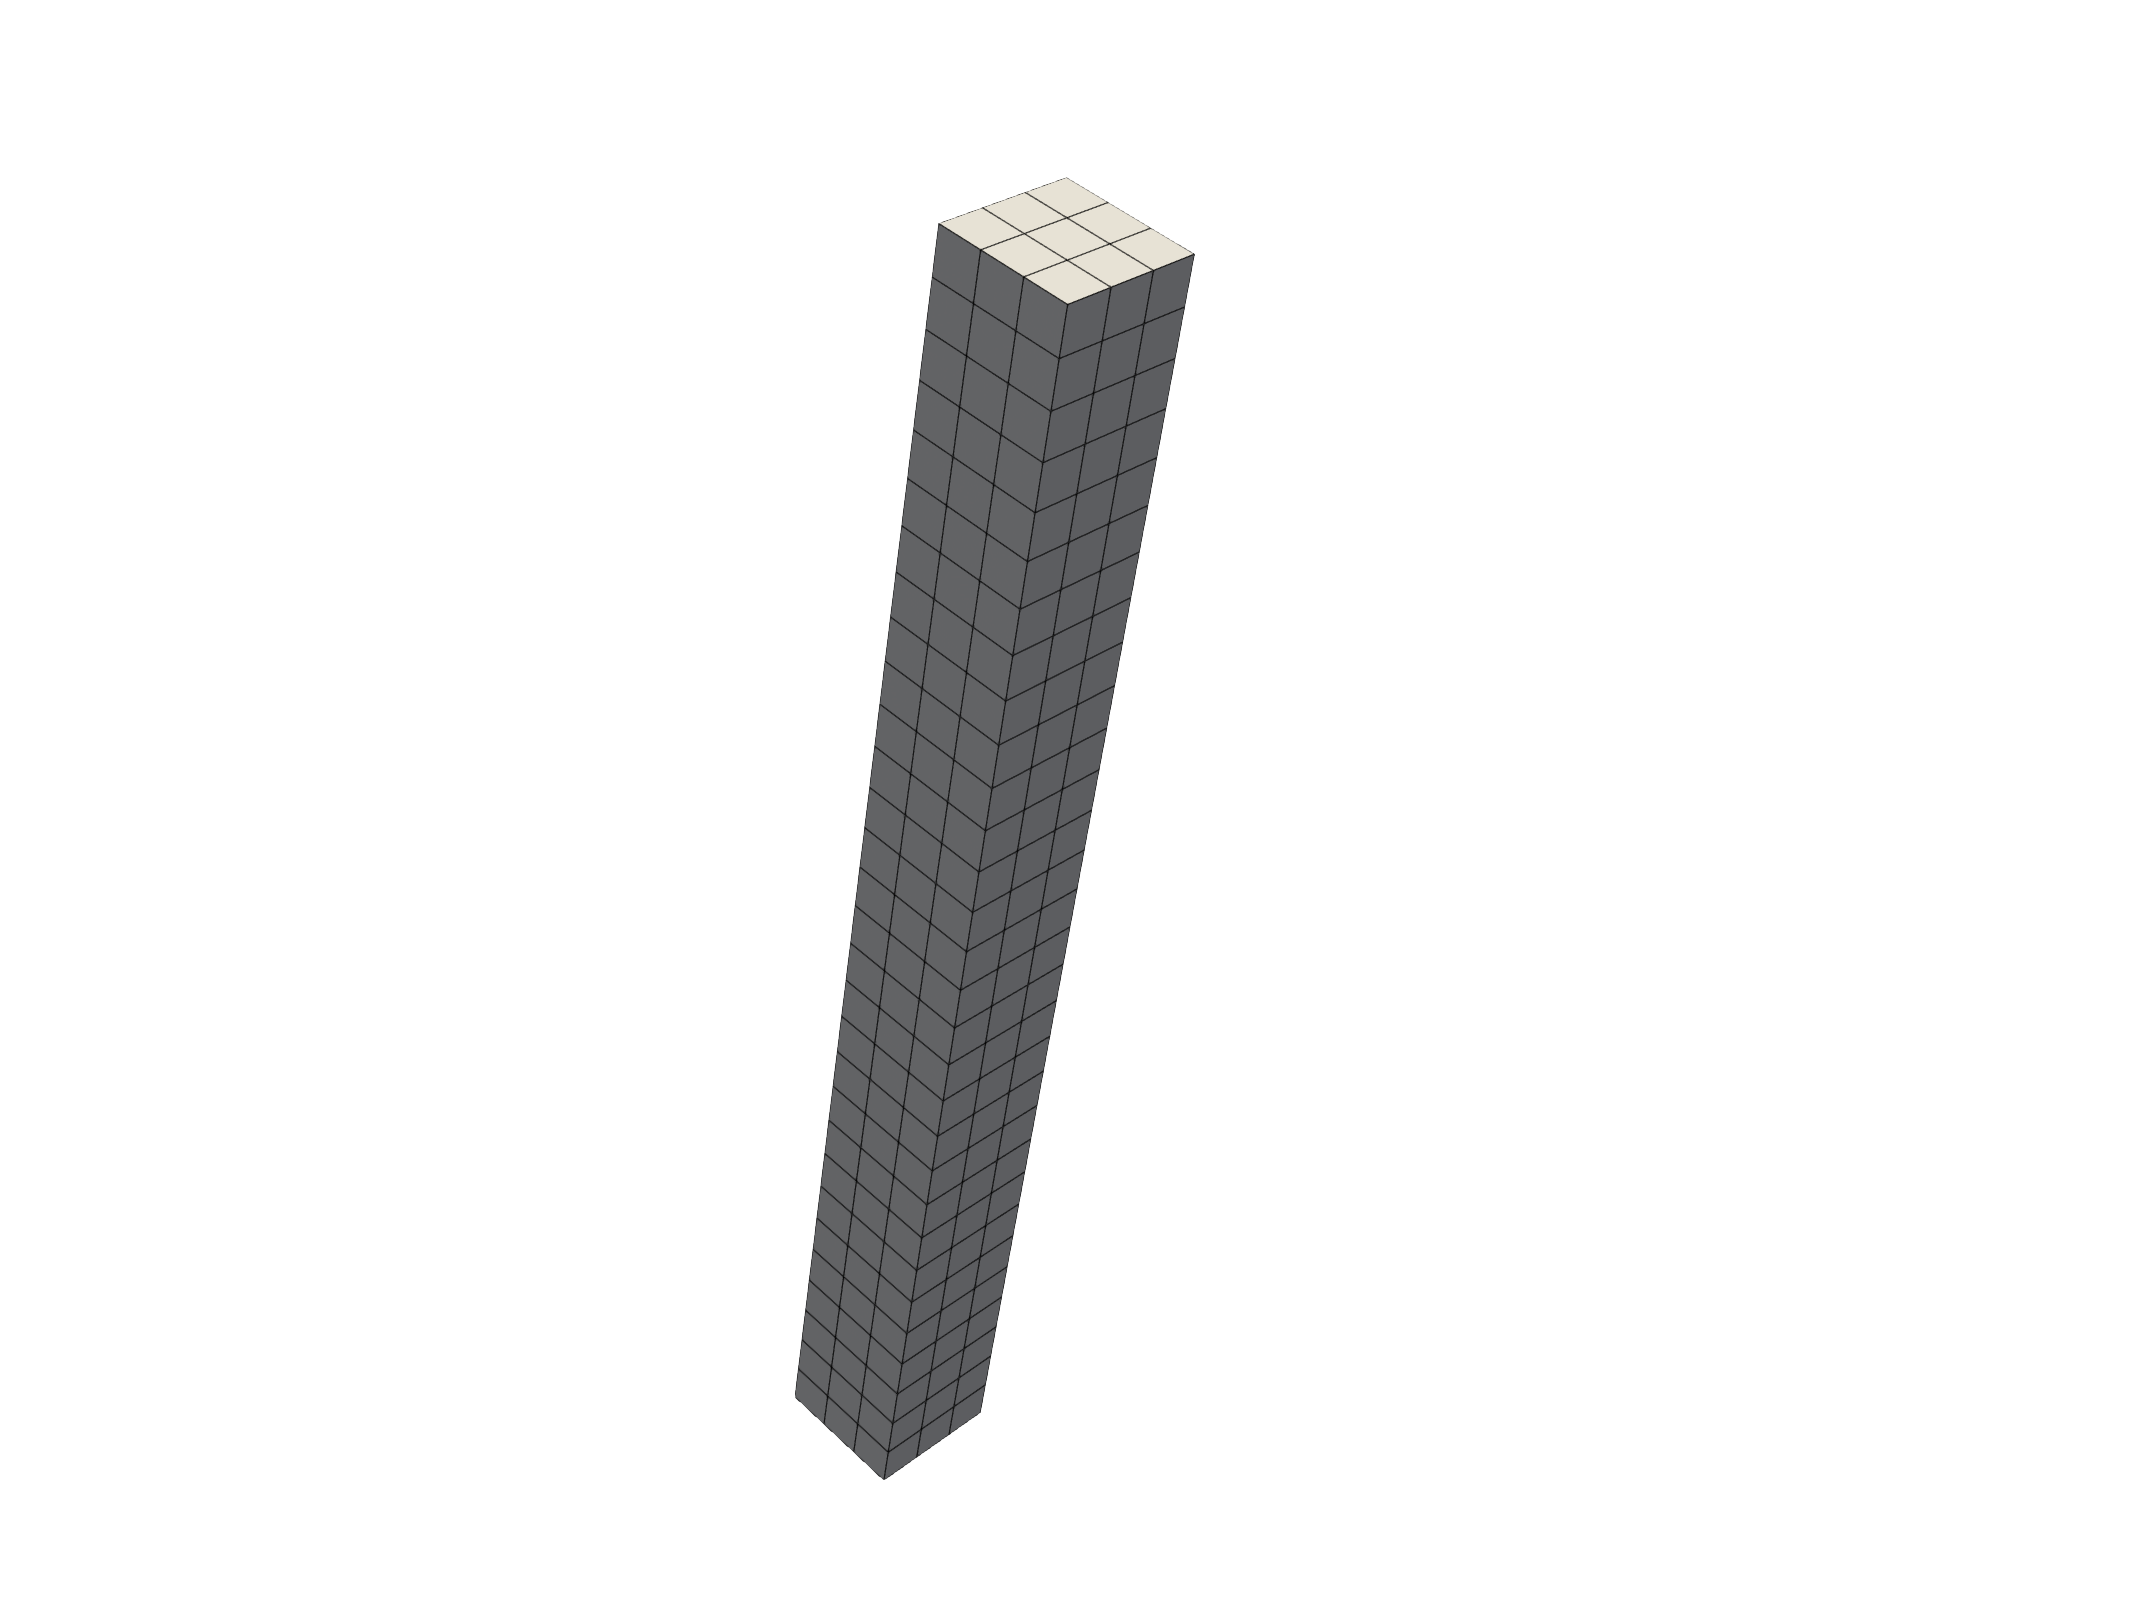
\includegraphics[width=0.5\textwidth]{figures/cantilever} 
	\subfigure[Displacement magnitude for t = $\left\{0, \, 0.1, \, 0.2\right\}$ s (translucent) and t = $\left\{0.3, \, 0.4, \, 0.5 \right\}$ s (opaque) for the mesh with $138\,240$ cells]
	{
	   \includegraphics[width=0.5\textwidth]{figures/cantilever_deformed}
   	} \quad
	\subfigure[Displacement magnitude of the centre of the upper surface of the beam vs time]
	{
	   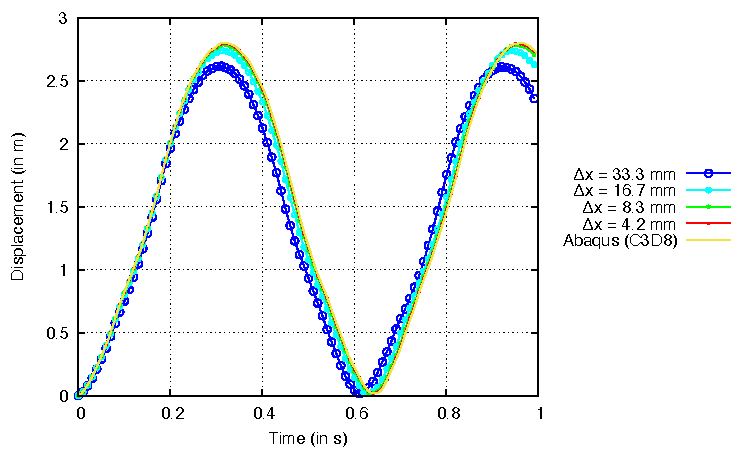
\includegraphics[width=0.6\textwidth]{figures/cantilever_disp} 
   	   %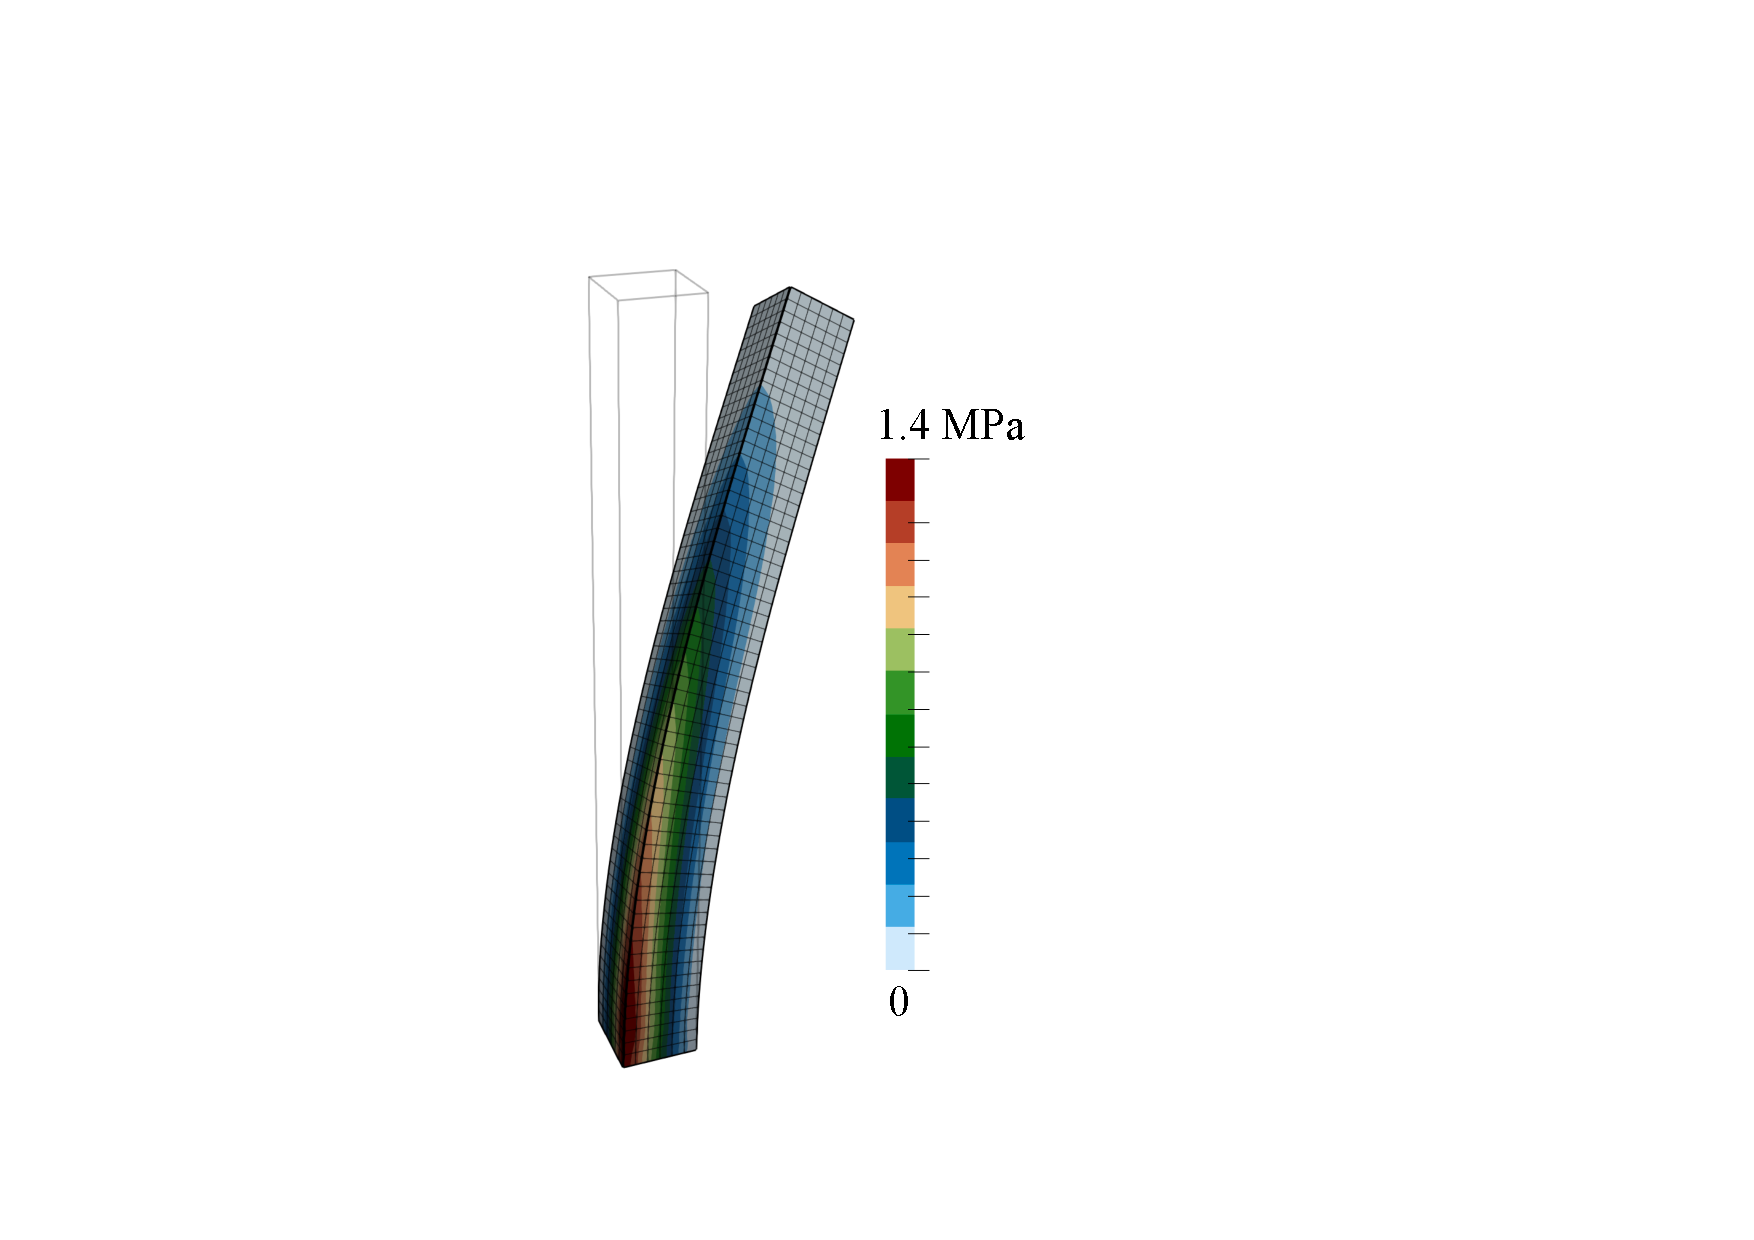
\includegraphics[height=0.45\textwidth]{figures/cantilever_sigmaEq}  
   	}
   \caption{Deflection of a 3-D Cantilevered Beam}
   \label{fig:dynamic_cantilever}
\end{figure}
%\hl{It would be good to add a reference results, e.g. from FE}

%\begin{figure}[htbp]
%   \centering
%   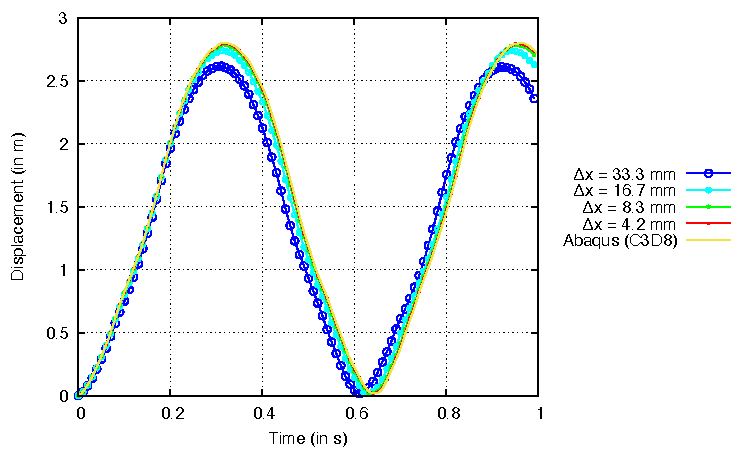
\includegraphics[width=0.55\textwidth]{figures/cantilever_disp} 
%%	\subfigure[Deflection vs time for the four meshes using a time step of 0.001617274174 s]
%%	{
%%   		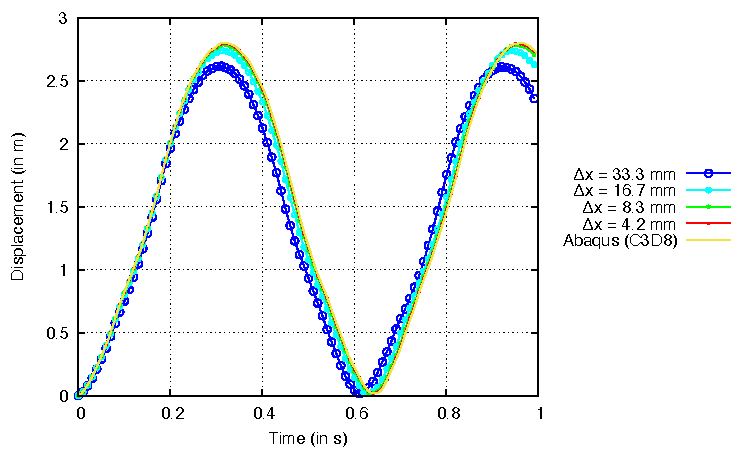
\includegraphics[width=0.55\textwidth]{figures/cantilever_disp} 
%%   	}
%%	\subfigure[XXX]
%%	{
%%   		
\includegraphics[width=0.25\textwidth]{figures/placeholder}  
%%   	}
%   \caption{Vibration of a 3-D Cantilevered Beam case}
%   \label{fig:dynamic_cantilever_results}
%\end{figure}

%\hl{maybe we should state the nonlinear/linear solver settings for completeness}


\paragraph{Case 7: Axial Turbine Blade}
This 3-D, quasi-static, small strain, linear elastic case consists of a twisted axial turbine blade (Figure \ref{fig:turbine_blade}) with the Cartesian axis-aligned bounding box $105.55\times177.628\times336.5$ mm.
This case demonstrates the application of the proposed approach to an industrially-relevant geometry.
The blade is constrained at the rotation axis end and subjected to a centrifugal body force $\bb{f}_b = \rho \omega^2 \bb{r}$ kg m$^{-2}$ s$^{-2}$.
The scalar rotational velocity $\omega = \frac{2\pi \text{RPM}}{60}$ is defined here about the $x$ axis, where $\text{RPM} = 720$.
The vector $\bb{r}$ is defined as the shortest vector to the rotation ($x$) axis.
The blade's root is constrained, while all other surfaces are traction-free.
A linear elastic material is assumed with $E = 4.431$ GPa, $\nu = 0.33$, and $\rho = 1200$ kg m$^{-3}$.
% while the area $A = (0.2)(0.2) = 0.04$ m$^2$ and the second moment of area $I = 0.0001333$ m$^4$.
An unstructured polyhedral mesh with $322\,161$ cells is employed (Figure \ref{fig:turbine_blade}), created in Ansys Fluent and converted to the OpenFOAM format using the \texttt{fluent3DMeshToFoam} OpenFOAM utility.
\hl{Could we include a finer mesh?}
%A fixed time step size of \hl{XXX} s is chosen, corresponding to a \hl{YY} on the coarsest mesh \hl{update as required}.
%The total time period is \hl{XXX} s, corresponding to \hl{XX} expected oscillation periods.
%\hl{An advantage of this case over the cantilever is that it is complex geometry; a disadvantage is that we do not have a reference solution}
%\hl{A mitigation for this disadvantage is we could run it in Abaqus to provide a credible reference}
\begin{figure}[htbp]
   \centering
%   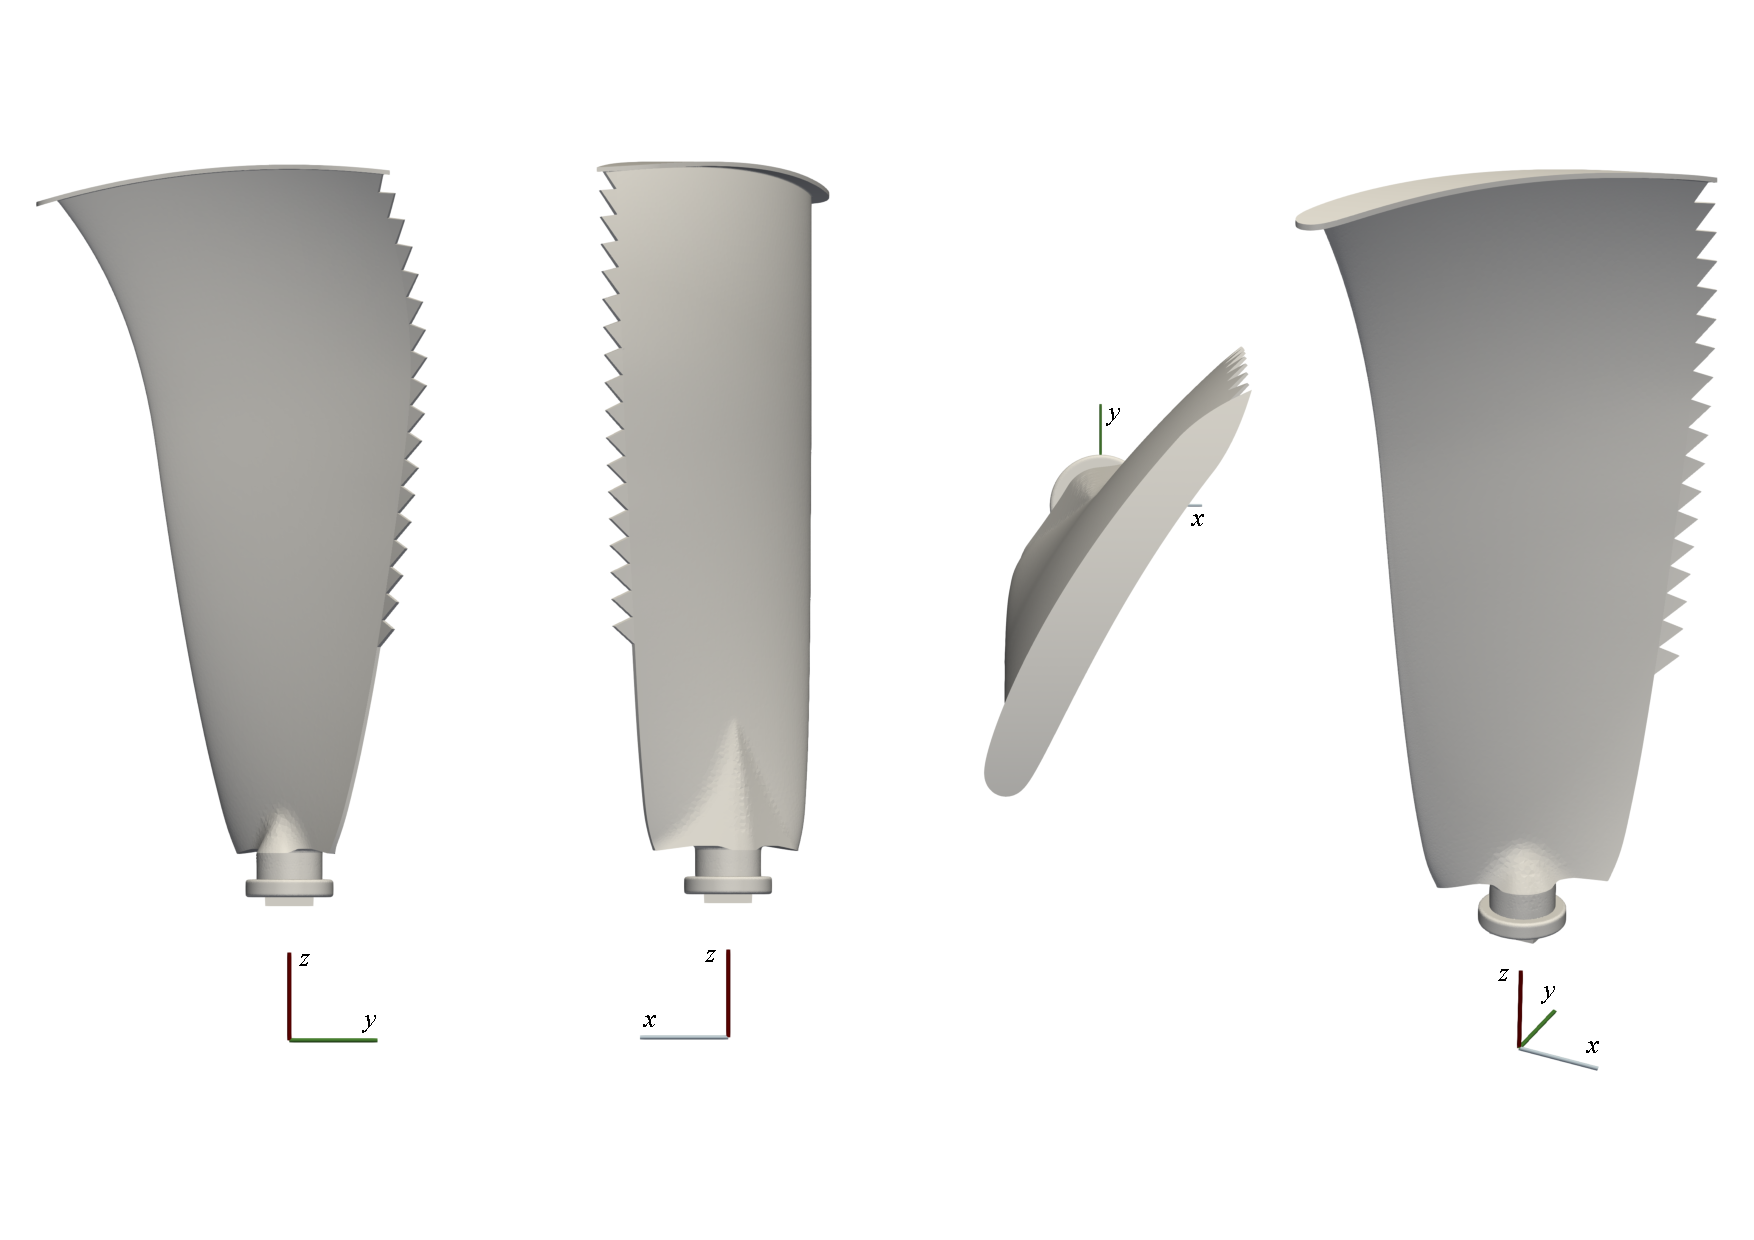
\includegraphics[width=\textwidth]{figures/turbine_blade_geometry.pdf} 
   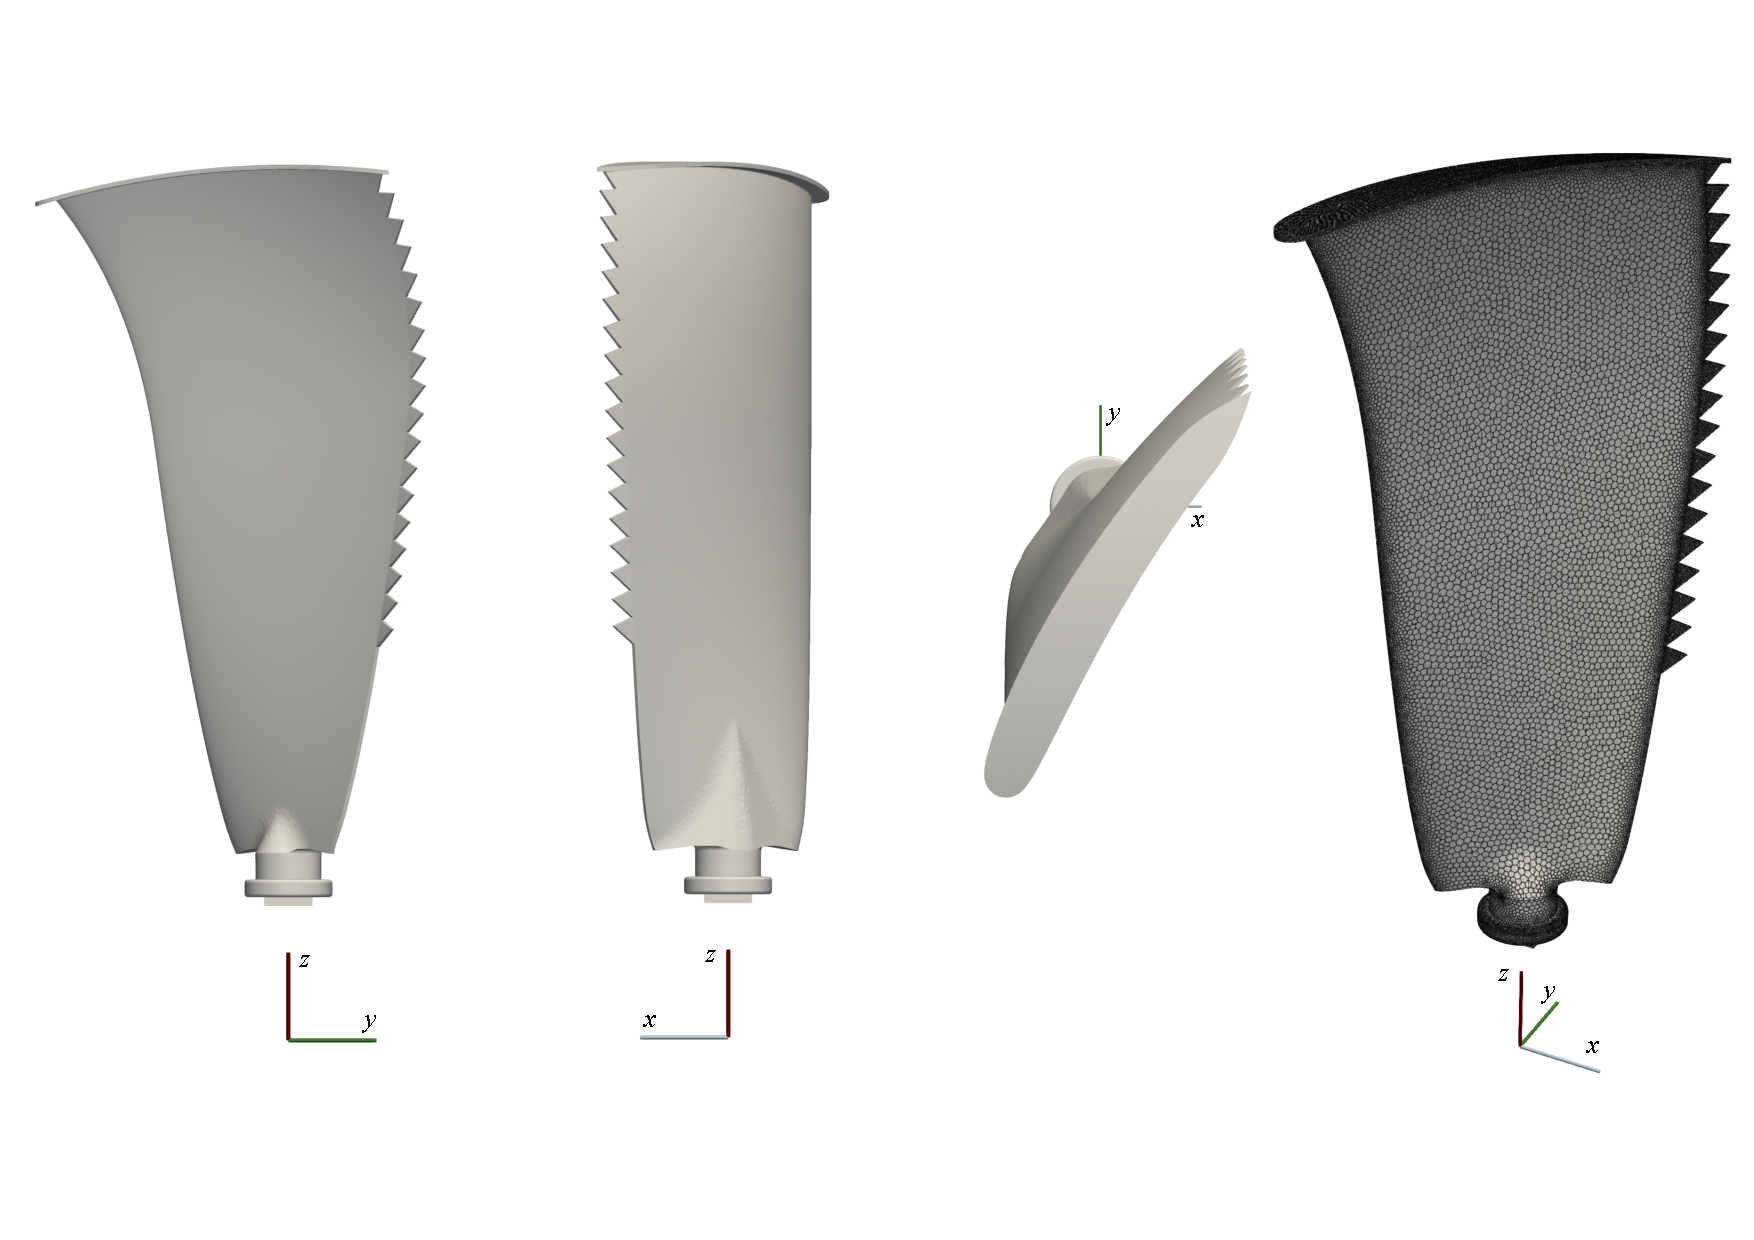
\includegraphics[width=\textwidth]{figures/turbine_blade_geometry_mesh.pdf} 
   \caption{Axial turbine blade case geometry}
   \label{fig:turbine_blade}
\end{figure}

The prediction displacement magnitude distribution (left image in Figure \ref{fig:turbine_blade_disp_sigmaEq}) is consistent with a cantilever with the largest deflection occurring at the distal free-end of the turbine.
The equivalent (von Mises) stress distribution (right image in Figure \ref{fig:turbine_blade_disp_sigmaEq}) shows the peak stresses to occur near the blade root and leading and trailing edges, with concentrations near the trailing edge vortex generators \hl{correct name?}.
\begin{figure}[htbp]
   \centering
   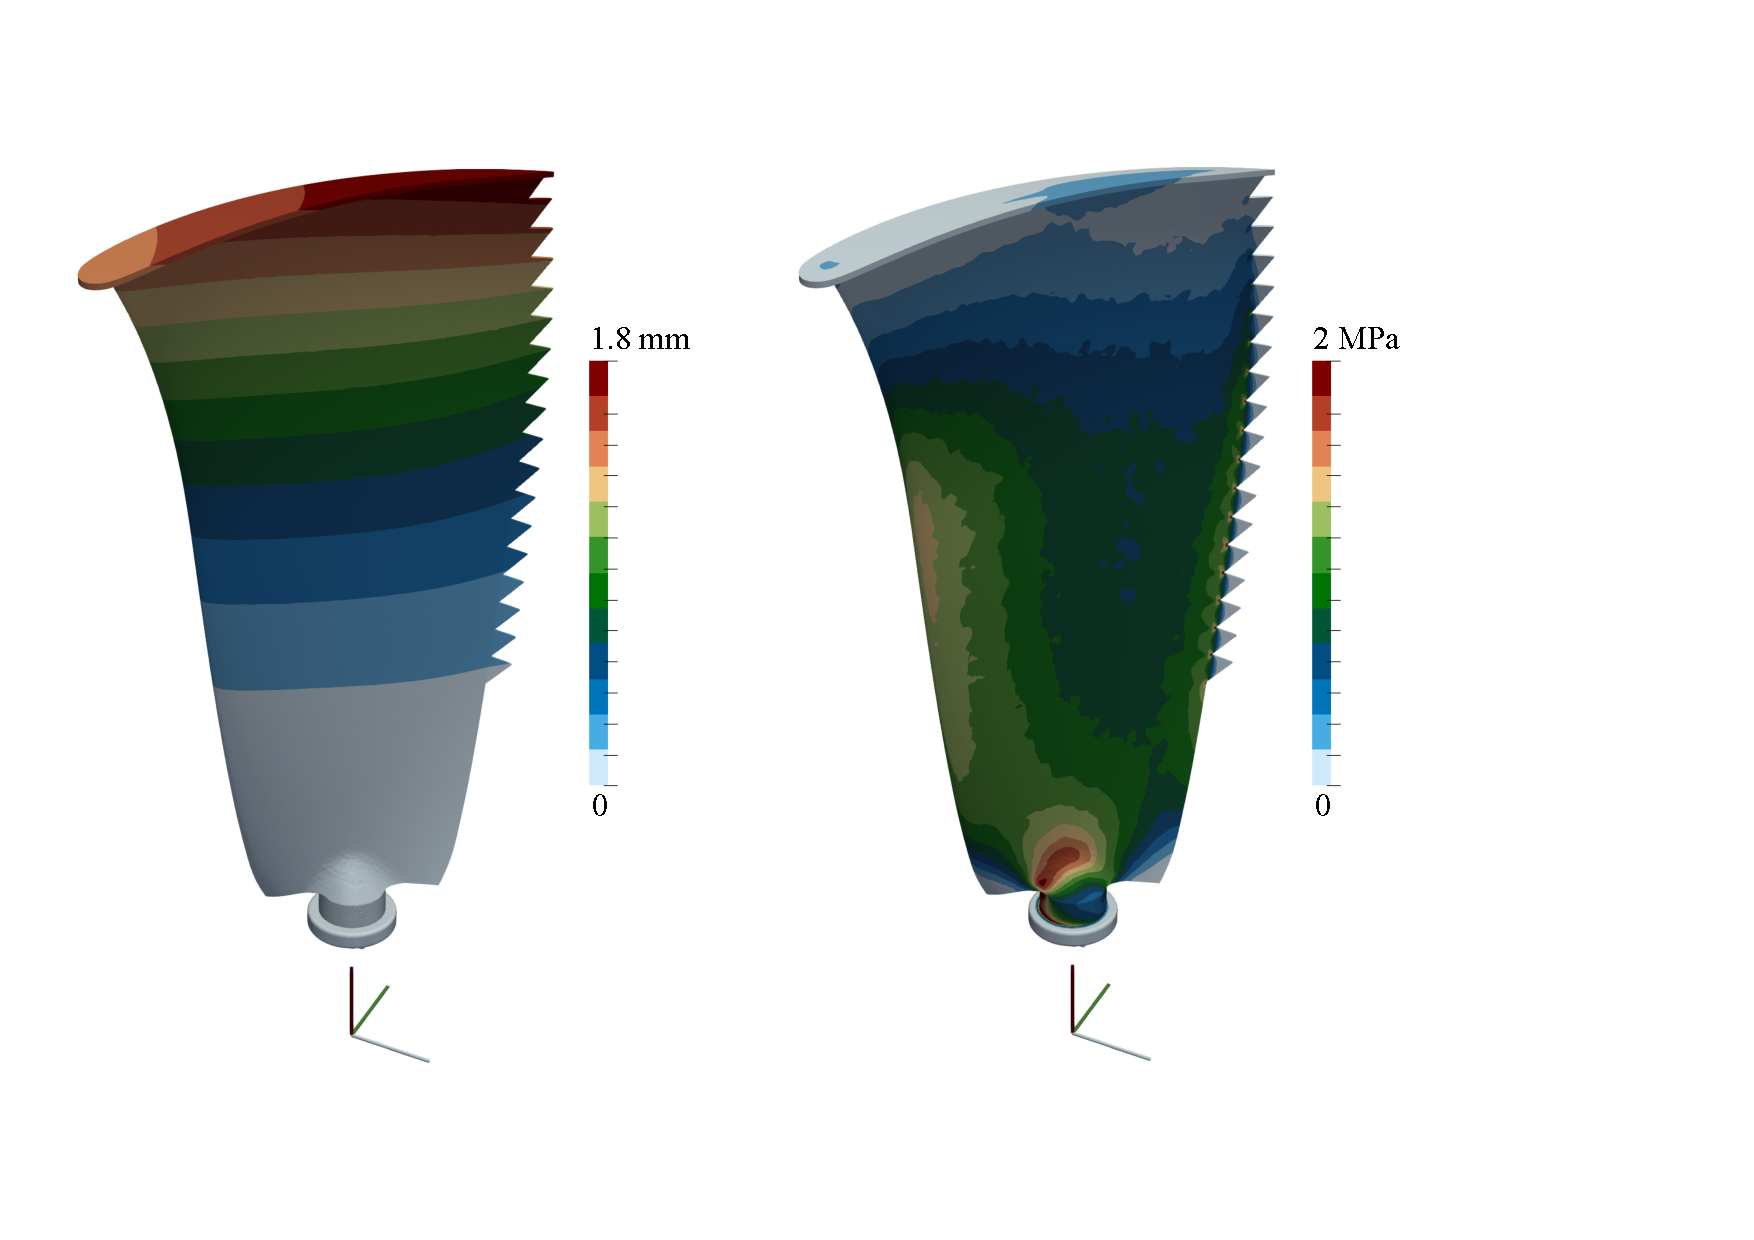
\includegraphics[width=0.8\textwidth]{figures/turbine_blade_disp_sigmaEq.pdf} 
   \caption{Axial turbine blade displacement magnitude and equivalent stress distributions \hl{non-smooth stress contours => indicative of low order of accuracy}}
   \label{fig:turbine_blade_disp_sigmaEq}
\end{figure}



\paragraph{Case 8: Elastic plate behind a rigid cylinder}
\citet{Turek2006} proposed this well-known fluid-solid interaction benchmark case as an extension of the classic flow around a cylinder in a channel problem \cite{Ferziger2002}.
The \texttt{FSI3} variant of the case examined here (Figure \ref{fig:hronTurek-mesh}) consists of a horizontal channel (0.41 m in height, 2.5 m in length) with a rigid cylinder of radius 0.05 m, where the cylinder centre is 0.2 m from the bottom and inlet (left) boundaries.
A parabolic velocity is prescribed at the inlet velocity with a mean value of 2 m/s.
A St.\ Venant-Kirchhoff hyperelastic plate ($E = 5.6$ MPa, $\nu = 0.4$) of 0.35 m in length and 0.02 m in height is attached to the right-hand side of the rigid cylinder.
The fluid model is assumed to be isothermal, incompressible, and laminar and adopts the segregated PIMPLE solution algorithm.
The fluid's kinematic viscosity is 0.001 m$^2$/s and density is 1000 kg/m$^3$, while the solid's density is $10\,000$ kg/m$^3$.
The interface- quasi-Newton with inverse Jacobian from a least-squares model coupling approach \cite{Degroote2009} is employed for the fluid-solid interaction coupling.
The fluid-solid interface residual is reduced by four orders of magnitude within each time step.
Further details of the fluid-solid interaction procedure are found in \citet{Tukovic2018a}.
%\begin{figure}[htbp]
%   \centering
%%	\subfigure[Geometry (taken from \citet{Tukovic2018a})]
%%	{
%	   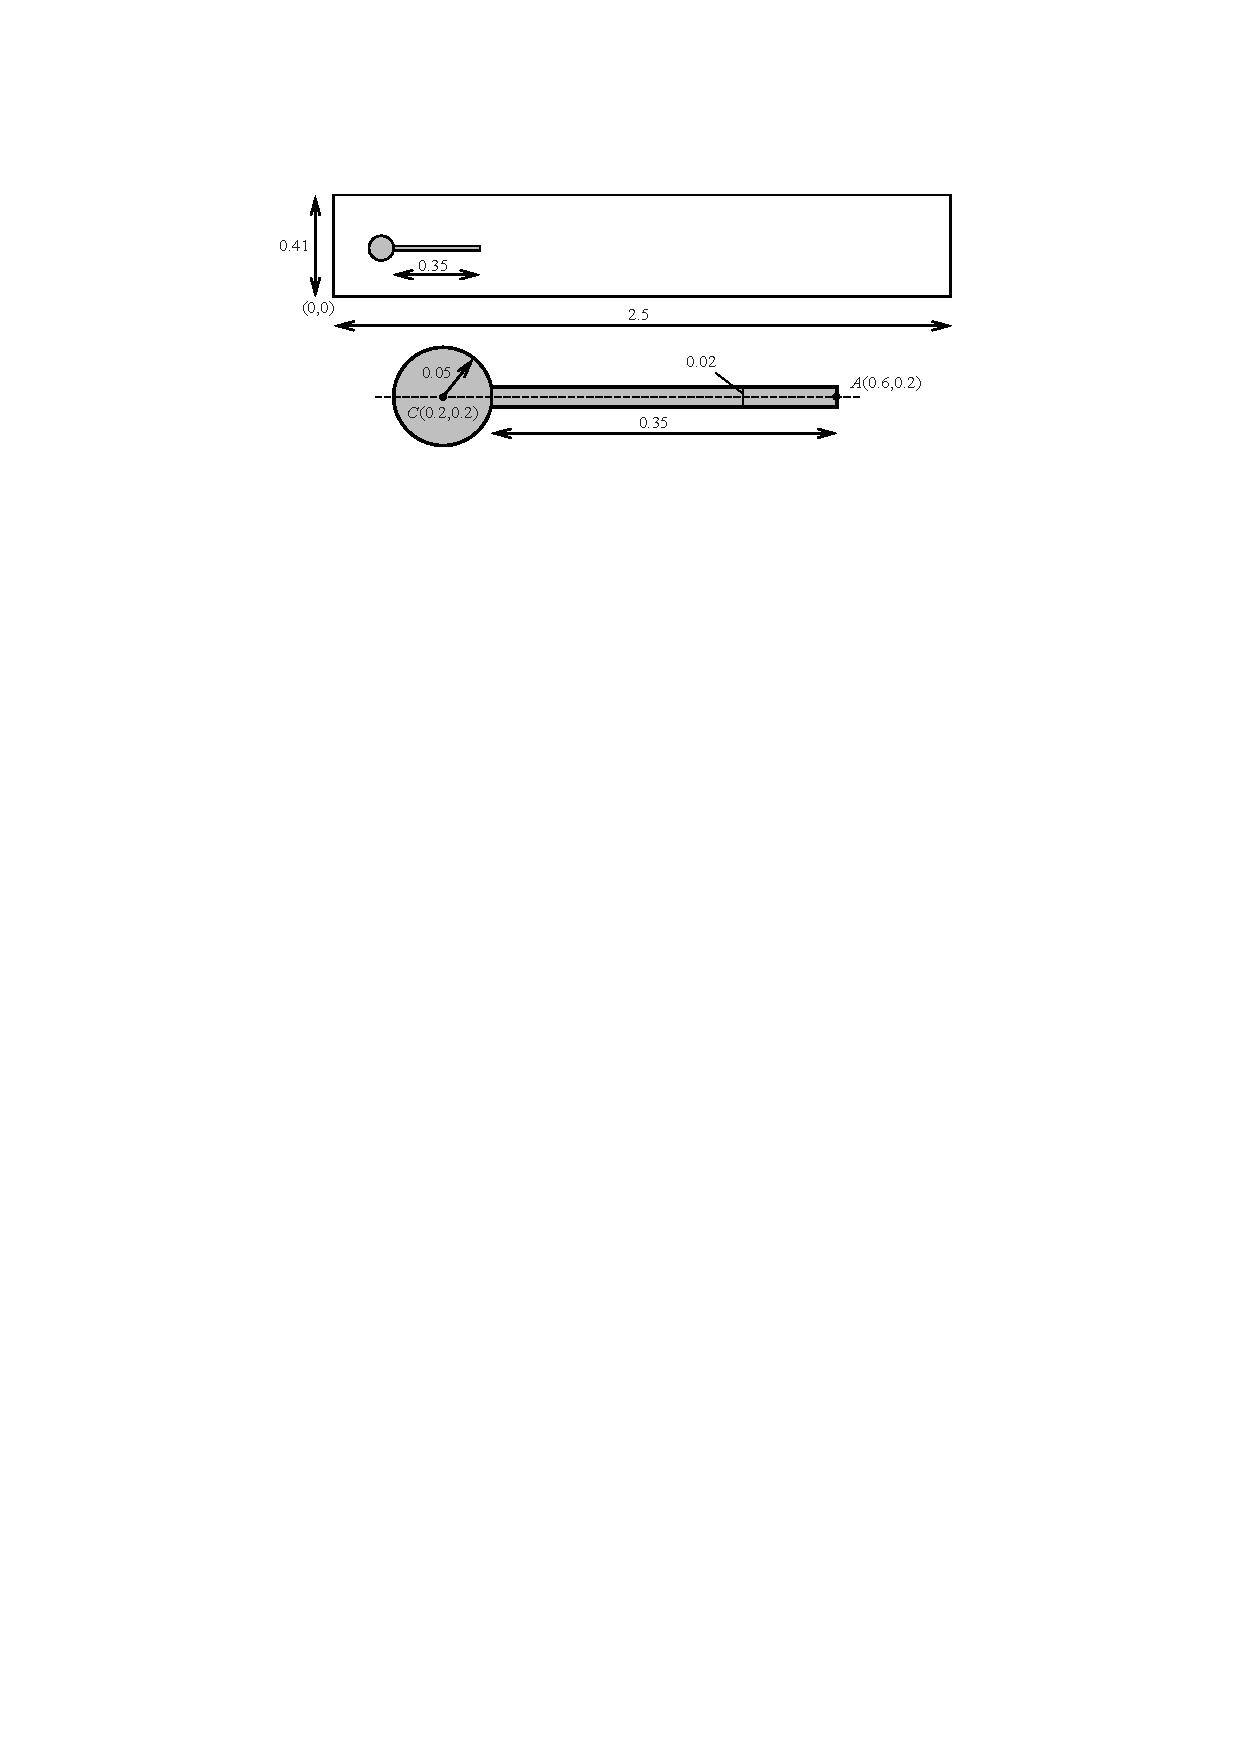
\includegraphics[width=0.7\textwidth]{figures/hronTurek-geometry} 
%%   	}
%   \caption{Elastic plate behind a rigid cylinder case geometry and mesh}
%   \label{fig:hronTurek-geometry}
%\end{figure}
Three successively refined quadrilateral meshes are employed:
The fluid region meshes have $1\,252$, $5\,008$, and $20\,032$ cells, while the solid region meshes have 156,  624 and $2\,496$ cells.
The total simulation time is 20 s, and the time-step size is 0.5 ms. 
\begin{figure}[htbp]
   \centering
	\subfigure[Mesh containing $5\,336$ cells in the fluid region and 630 cells in the solid region, where a closeup of the plate is shown in the right]
	{
   		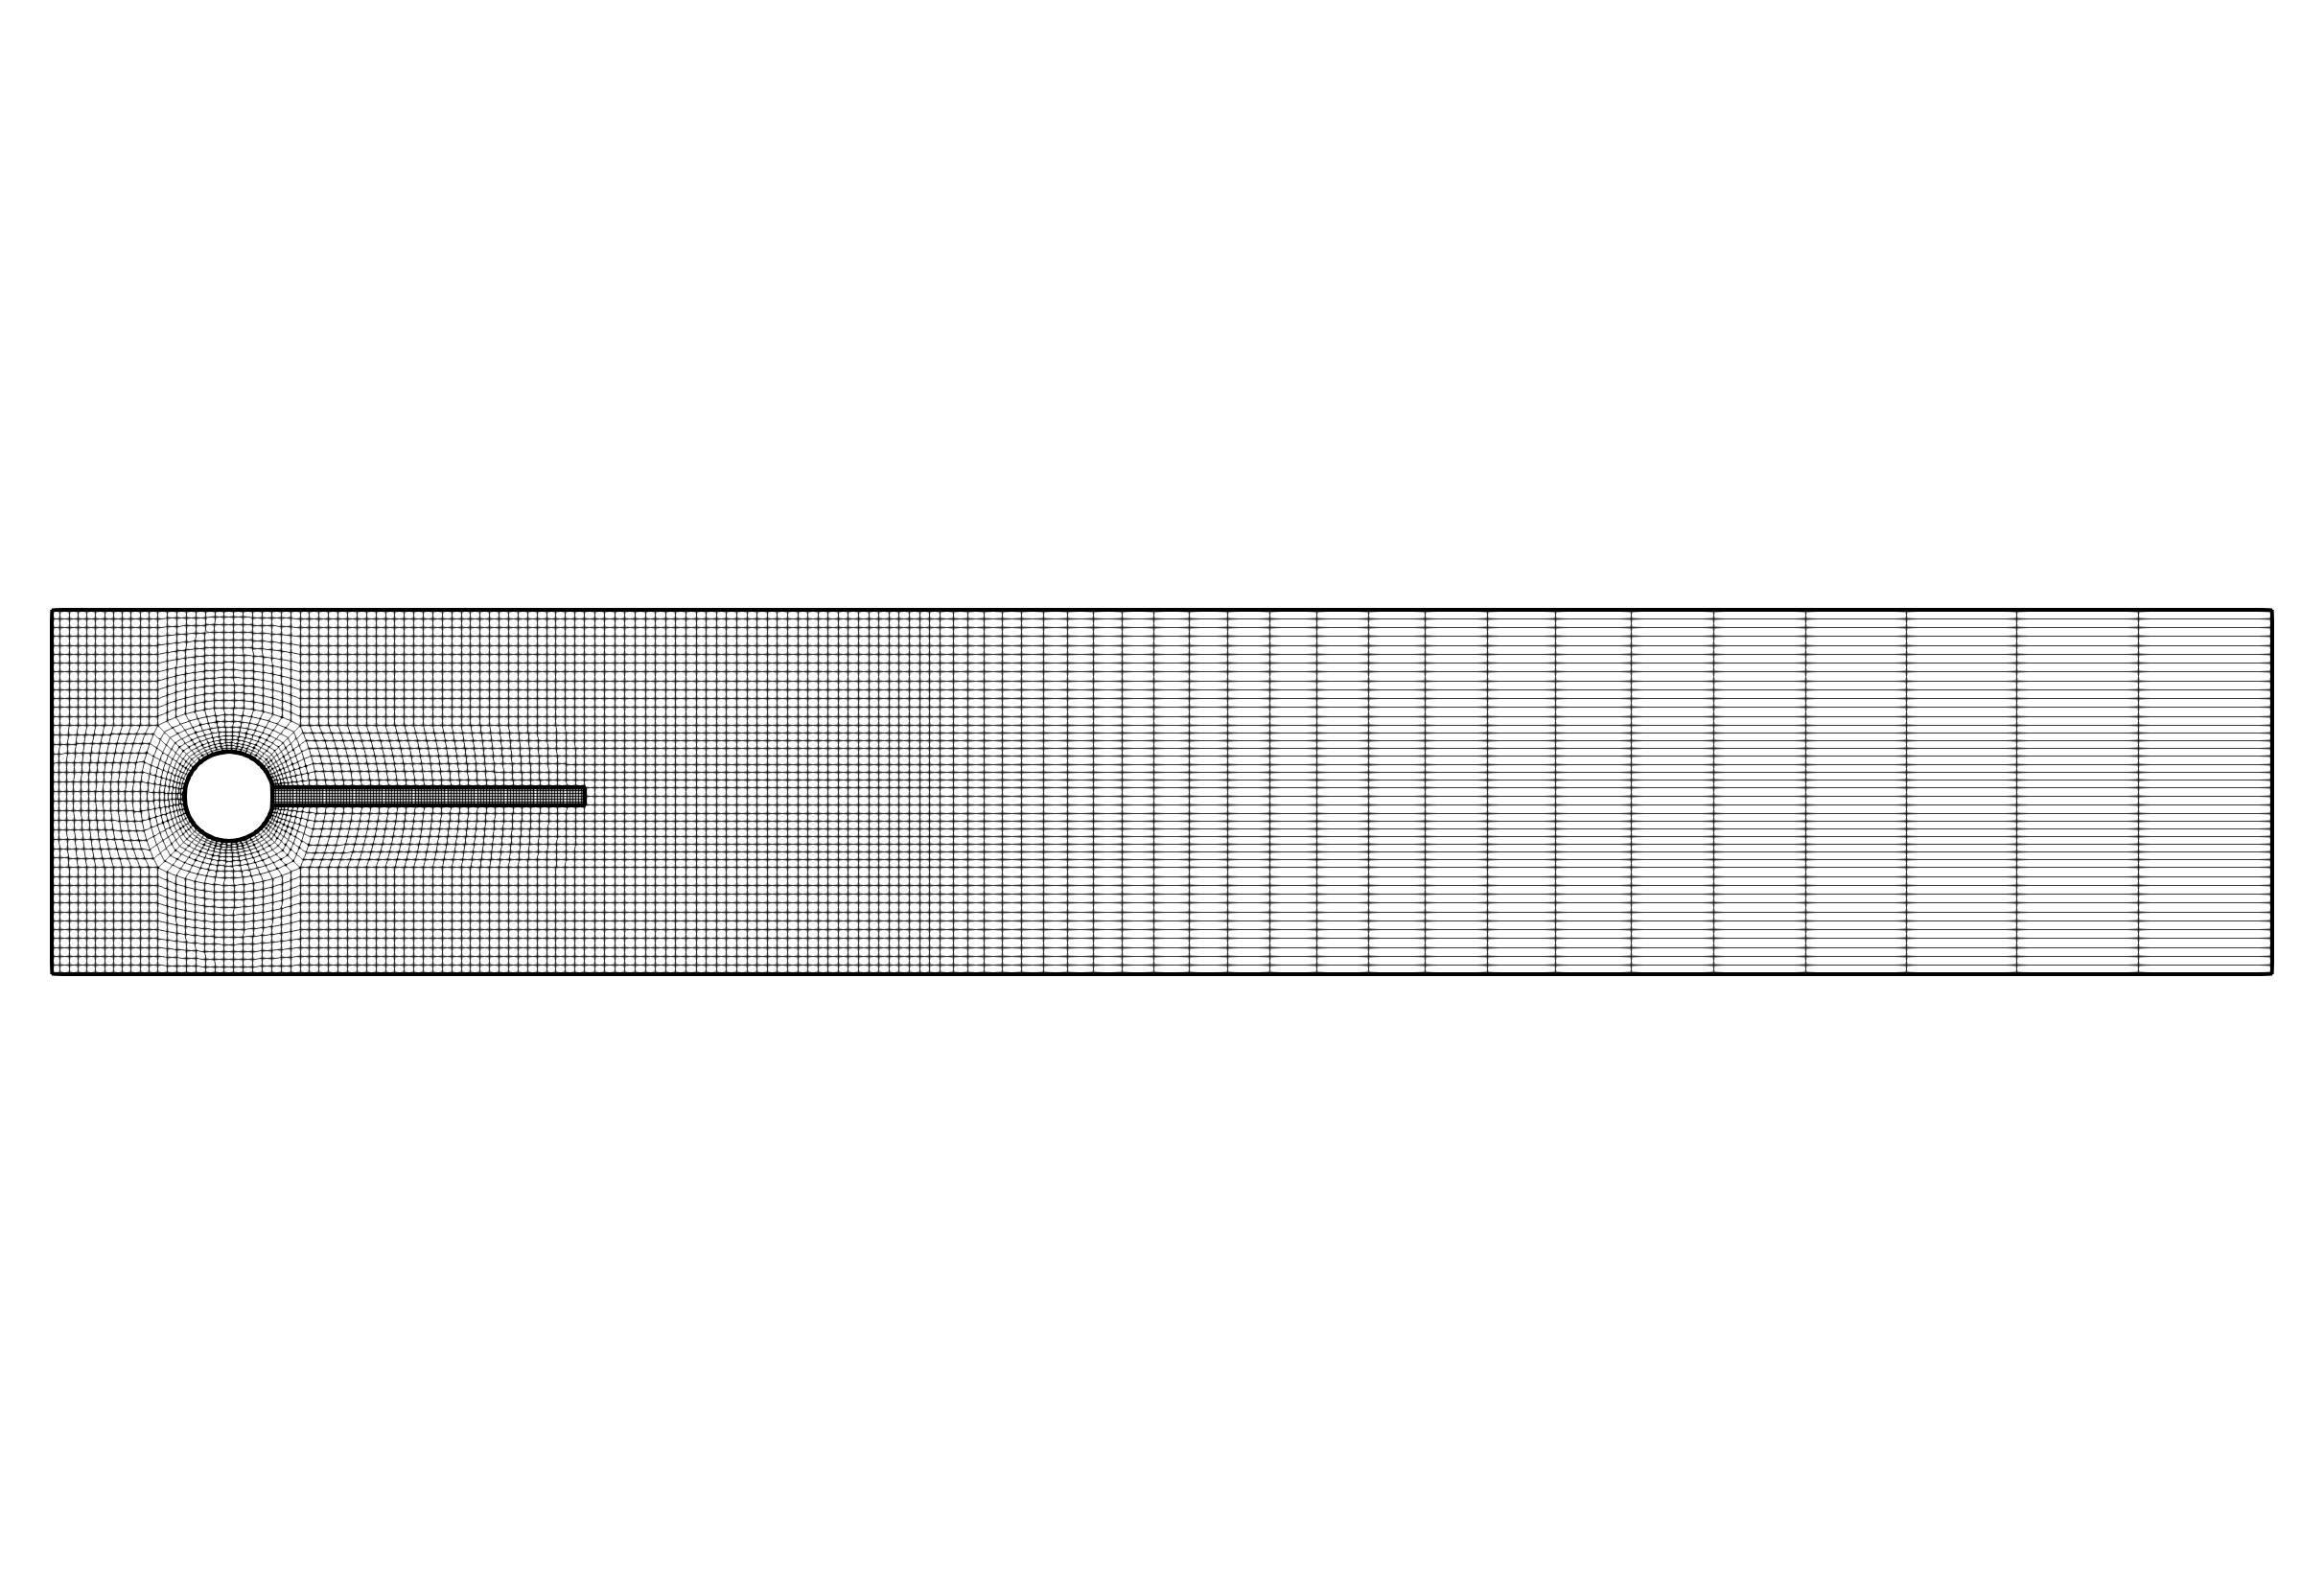
\includegraphics[width=0.7\textwidth]{figures/hronTurek-mesh}
	}
	\subfigure[Close-up of the mesh around the plate]
	{
   		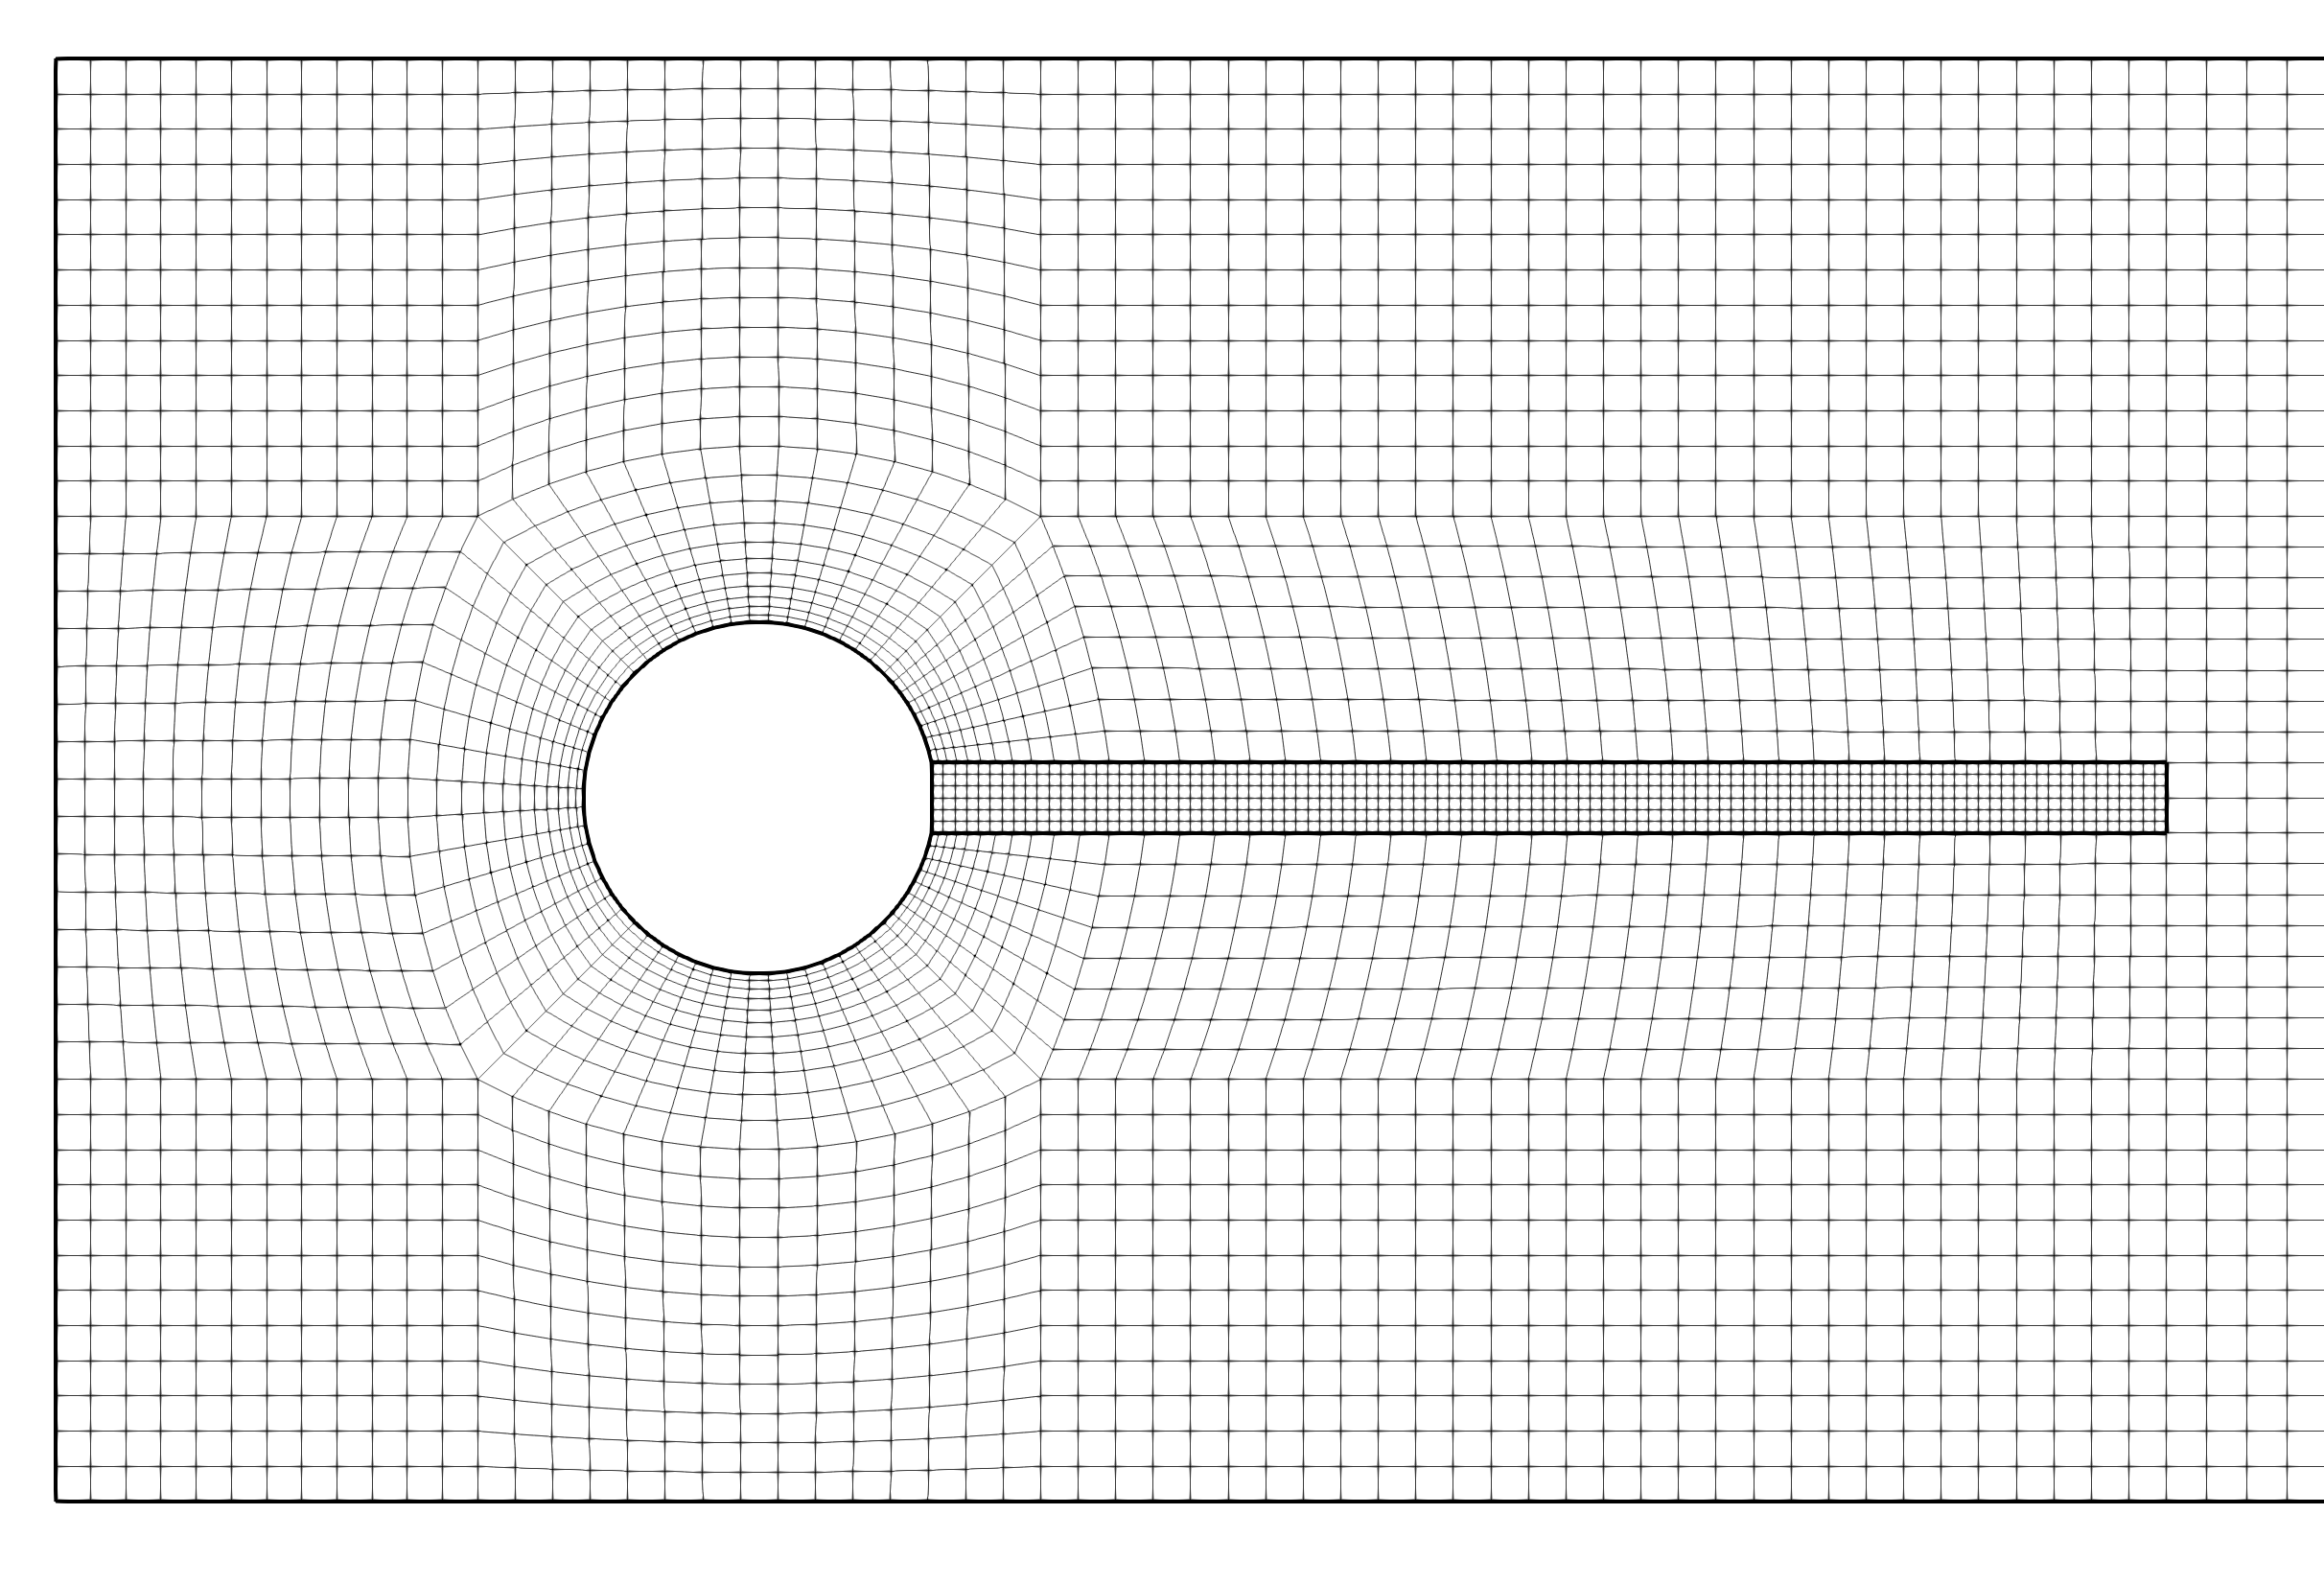
\includegraphics[width=0.4\textwidth]{figures/hronTurek-mesh-zoom}  
   	}
   \caption{Elastic plate behind a rigid cylinder case geometry and mesh}
   \label{fig:hronTurek-mesh}
\end{figure}

Figure \ref{fig:hronTurek-results} shows the velocity field in the fluid region and displacement magnitude in the solid region at $t = 4.42$ s, corresponding to a peak in the vertical displacement of the plate free-end oscillation.
The fluid is seen to accelerate as it passes the cylinder, with regular vortices being thrown off the plate, causing it to oscillate.
\begin{figure}[htbp]
   \centering
	   \includegraphics[width=\textwidth]{figures/hronTurek-results} 
%	\subfigure[Velocity field in the fluid region and displacement magnitude in the solid region at $t = 4.42$ s]
%	{
%	   \includegraphics[width=0.8\textwidth]{figures/hronTurek-results} 
%   	}
%	\subfigure[Vertical displacement of the end of the plate vs time]
%	{
%   		\includegraphics[width=0.3\textwidth]{figures/placeholder}  
%   	}
   \caption{Elastic plate behind a rigid cylinder case results at $t = 20$ s for the mesh with $20\,032$ cells in the fluid region and $2\,496$ in the solid region. The velocity magnitude is shown in the fluid region while the displacement magnitude is shown in the solid region.}
   \label{fig:hronTurek-results}
\end{figure}
The predicted mean, amplitude and frequency of the vertical and horizontal displacement of the end of the plate are compared with the results from \citet{Turek2006} in Table \ref{tab:hronTurekDisp}.
As directed in \citet{Turek2006}, the maximum and minimum values for the last period are used to calculate the mean and amplitude:
\begin{eqnarray}
	\text{mean} = \frac{1}{2}(\text{max} + \text{min}), \quad\quad
	\text{amplitude} = \frac{1}{2}(\text{max} - \text{min})
\end{eqnarray}
while the frequency is calculated as the inverse of the period.
\begin{table}[htb]
	\centering
		\begin{tabular}{lll}
			\hline
			Mesh (number of fluid and solid cells) & $u_x$ (in mm) & $u_y$ (in mm) \\
			\hline
			%  \hl{This data is taken as the average from 4-6 seconds: I am now running the case up to 20 seconds as per the benchmark}
%			1 ($1\,252$ + 156)  & $-0.1 \pm 0.01 \,[ 18.5 ]$ & $1.60 \pm 0.20 \,[ 5.5 ]$ \\
%			2 ($5\,008$ + 624)  & $-2.13 \pm 2.07 \,[ 11 ]$ & $2.00 \pm 28.84 \,[ 5.5 ]$ \\
%			3 ($20\,032$ + $2\,496$)  & $-2.62 \pm 2.46 \,[11]$ & $1.80 \pm 32.01 \,[ 5.5 ]$ \\
			% Data below is from the last cycle in the case run up to 20 s
			1 ($1\,252$ + 156)  & $ -0.1 \pm 0.001 \,[ 47.6 ]$ & $1.58 \pm 0.002 \,[ 5.88 ]$ \\
			2 ($5\,008$ + 624)  & $-2.16 \pm 2.00 \,[ 10.2 ]$ & $1.54 \pm 29.56 \,[ 5.6 ]$ \\
			3 ($20\,032$ + $2\,496$)  & $-2.51 \pm 2.37 \,[12.1]$ & $0.87 \pm 33.08 \,[ 5.6 ]$ \\
			\hline
			\citet{Turek2006} & $-2.69 \pm 2.53\,[10.9]$ & $1.48 \pm 34.38\,[5.3]$ \\
			\hline
		\end{tabular}
	\caption{Average predicted displacements (mean $\pm$ amplitude $[$frequency$]$) of the free end of the plate. Note that large-scale plate oscillations in mesh 1 (coarsest mesh) die out within the first 10 s.}
%	 \hl{Hron-Turek say to use the last cycle, but surely taking the average of cycles would be better for benchmarking...} \hl{e.g. the average of the mesh 3 cycle is slightly lower than the rest} \hl{we could also report the average}
		\label{tab:hronTurekDisp}
\end{table}


%%--------------------------------------------------------------------------------------------------------------------%%
\subsection{Robustness and Resource Requirements}
\label{sec:resource_requirements}
%%--------------------------------------------------------------------------------------------------------------------%%
This section compares the robustness and resource requirements of the Jacobian-free Newton-Krylov and segregated approaches on the cases presented in Section \ref{sec:accuracy}.
Specifically, cases where either approach diverges are examined, and the time and memory requirements are presented.
In some cases, time and memory requirements from finite element software Abaqus are given for reference.
Time and memory requirements are implementation and hardware-specific; nonetheless, it is insightful to see the relative performances of the Jacobian-free Newton-Krylov and segregated approaches on the same hardware and within the same implementation framework.
% where several mesh densities are examined.
%Time and memory requirements from the classic segregated approach are given for comparison, along with the requirements from commercial finite element software Abaqus (version XXX): \hl{ask Dylan to create the Abaqus results when we are happy the paper will not change}.
%The finite element approach uses a coupled solution algorithm and direct linear solver, where a Newton-Raphson method is used for resolving nonlinearities.
%\hl{Take care when comparing times between different hardware}

Table \ref{tab:times_memory} lists the wall clock times (time according to a clock on the wall, rounded to the nearest second) and maximum memory usage according to the GNU time utility.
All clock times and memory usage were generated using a Mac Studio with an M2 Ultra CPU on one CPU core, where the code was built with the Clang compiler.
%\hl{Present data for one hardware first, and give comparison after.}
Examination of multi-CPU-core parallelisation is left to Section \ref{sec:parallelisation}.
\begin{table}[!htb]
	\centering
		\begin{tabular}{ll|ll|ll}
			\hline
			\textbf{Case} & \textbf{Cell Count} & \multicolumn{2}{c|}{\textbf{JFNK}} & \multicolumn{2}{c}{\textbf{Segregated}} \\
			     &            & \textbf{Time} & \textbf{Memory} & \textbf{Time} & \textbf{Memory} \\
			     &            & (in s) & (in MB) & (in s) & (in MB) \\
			\hline 
			\textbf{MMS} & 384 & 0 & $78$ 				& 0 & 79 \\
			\emph{2-D, static,}	& $4\,374$ & 0 & $86$ 			& 0 & 94 \\
			\emph{linear elastic} & $41\,154$ & 1 & $195$  		& 2 & 181 \\
				&  $355\,914$ & 4 & $1\,063$ 		& 9 & $1\,289$ \\
				& $2\,958\,234$ & 41 & $6\,724$ 	& 92 & $6\,174$ \\
				& $24\,118\,074$ & 486 & $30\,606$ & $1\,732$ & $30\,601$ \\
			\hline
			\textbf{Elliptic} & 45 & 0 & $72$ & 0 & 76 \\
			\textbf{Plate} & 472 & 0 & $78$ & 0 & 81 \\
			\emph{3-D, static,} & $4\,140$ & 1 & $153$ & 8 & 124 \\
			\emph{linear elastic} & $34\,968$ & 7 & $754$ & 149 & 660 \\
				& $287\,280$ & 95 & $3\,943$ & $2\,694$ & $3\,661$ \\
				& $2\,438\,242$ & 988 & $21\,884$ &  &  running (increase snes-max-funcs)\\
			\hline
			\textbf{T-member} & 624& 0 & 84 					&  1 & 85 \\
			\emph{3-D, static,} & $4\,992$ & 1 & 127 				&  7 &  141 \\
			\emph{linear elastic} & $39\,936$ & 10 & 557			& 133 & 723  \\
				& $319\,488$ & 154 & $4\,024$ 				&  & running  \\
				& $2\,555\,904$ & $1\,751$ & $22\,814$ 			&  &  \\
			\hline
			\textbf{Ventricle} & $1\,620$ & 54 & 133 				& & running \\
			\emph{3-D, static,}& $12\,960$ & 576 & 553 			& & \\
			\emph{hyperelastic} & $103\,680$ & $8\,362$ & $3\,435$ 	& & \\
				& $829\,440$ & $150\,023$ & $11\,746$ 			& & \\
			\hline
			\textbf{Membrane i} & 9 & 0 & 77 	& 0 & 76 \\
			\emph{2-D, static,}& 36 & 0 & 77  	& 0 & 76 \\
			\emph{linear elastic}& 144 & 0 & 78  & 0 & 78 \\
				& 576 & 0 & 82 				& 1 & 84 \\
				& $2\,304$ & 0 & 94 			& 4 & 102 \\
				& $9\,216$ & 1 & 152 		& 33 & 186 \\
				& $36\,864$ & 2& 497 		& & running \\
				& $147\,456$ & 10& $1\,461$ 	& & \\
			\hline
			\textbf{Membrane ii} & 9 & x & x 	& 1 & 78 \\
			\emph{2-D, static,} & 36 & x & x 	& 2 & 78 \\
			\emph{hyperelastic} & 144 & x & x 	& 5 & 80 \\
				& 576 & x & x 			& 26 & 91 \\
				& $2\,304$ & x & x 		& & running \\
				& $9\,216$ & x & x 		& & \\
				& $36\,864$ & x & x 		& & \\
				& $147\,456$ & & $x$ 	& & \\
			\hline
			\textbf{Membrane iii} & 9 & x & x 		& 3 & 78 \\
			\emph{2-D, static,} & 36 & x & x 		& 6 & 79 \\
			\emph{hyperelastoplastic}& 144 & x & x	& 27 & 82 \\
				& 576 & x & x			& & running \\
				& $2\,304$ & x & x 		& & \\
				& $9\,216$ & x & x 		& & \\
				& $36\,864$ & x & x 		& & \\
				& $147\,456$ & & $x$ 	& & \\
			\hline
			\textbf{Cantilever} & $270$ & 11 & 85 		& & all diverged \\
			\emph{3-D, dynamic,} & $2\,160$ & 71 & 181 	& & \\
			\emph{hyperelastic}& $17\,280$ & 854 & 752 	& & \\
				& $138\,240$ & $11\,800$ & $5\,790$ 	& & \\
			\hline
			\textbf{Turbine} & $322\,161$ & $2\,386$ & x & & decide on meshes \\
			\emph{3-D, static,} & & & & & \\
			\emph{linear elastic} & & & & & \\
			\hline
			\textbf{FSI} & $1\,252$ + 156 & $4\,265$ & 743 				& $4\,820$ & 752 \\
			\emph{2-D, dynamic,}	& $5\,008$ + 624 & $33\,366$ & 788 	& $46\,328$ & 786 \\
			\emph{hyperelastic} & $20\,032$ + $2\,496$ & $154\,237$ & 729 	& & \\
			\hline
		\end{tabular}
	\caption{Execution times and maximum memory usage for Jacobian-free Newton-Krylov (JFNK) and segregated methods. Resource requirements are shown for the following cases: manufactured solution (MMS), XX }
	\label{tab:times_memory}
\end{table}

\hl{Comment on: Robustness, Time, Memory}
\hl{Comment on the effect of items in list at the start of this section}

\hl{Give details of relevant numerical settings, e.g. linear solver, preconditioner, Rhie-Chow scaling, globalisation strategy: where best to say this...}.

The trends shown in Table \ref{tab:times_memory} are common to all typical modern computer systems, however, the exact values depend on the particular details of the CPU, the memory configuration and the operating system.
To highlight the effect of hardware specification, Table \ref{tab:times_memory_spec2} lists the time and memory usage for a different system: \hl{e.g. Mac M2/M3 seem to give excellent performance vs Meluxina AMD EPYC cores}.
\hl{Describe the difference, e.g. 2-3 faster but same memory usage}
\hl{Additional comments/insights, e.g. time trends are the same for both systems}
\hl{We could even include multiple systems here, e.g. Mac Studio vs Meluxina AMD vs Zagreb Intel workstation vs Intel i9/i7}
\begin{table}[htb]
	\centering
		\begin{tabular}{lllll}
			\hline
			Hardware & Case & Number of Cells & Time (in s) & Memory (in MB) \\
			\hline 
			Mac Studio, M2 Ultra & Spherical cavity & 1,234 & 345 & 1,234  \\
			Mac Studio, M2 Ultra & Spherical cavity & 12,345 & 345 & 1,234  \\
			Mac Studio, M2 Ultra & Spherical cavity & 123,456 & 345 & 1,234  \\
			Meluxina, AMD EPYC & Spherical cavity & 1,234 & 345 & 1,234  \\
			Meluxina, AMD EPYC & Spherical cavity & 12,345 & 345 & 1,234  \\
			Meluxina, AMD EPYC & Spherical cavity & 123,456 & 345 & 1,234  \\
			\hline
		\end{tabular}
	\caption{Execution times and maximum memory usage for \hl{Hardware Spec 2}}
	\label{tab:times_memory_spec2}
\end{table}


\hl{Mention cases that diverge using one or both approaches: JFNK -> plastic; seg -> ventricle}


%%--------------------------------------------------------------------------------------------------------------------%%
\subsection{Effect of Mesh Type}
%%--------------------------------------------------------------------------------------------------------------------%%
To highlight the effect of mesh type on the performance of the proposed Jacobian-free Newton-Krylov approach, case \hl{X} is re-examined using several mesh types:
(i) structured hexahedral; (ii) structured tetrahedral; (iii) unstructured tetehrahedral; and (iv) unstructured poyhedral.
%Pick one case and show its timings and memory for tet (Gmsh), hex and poly (Gmsh + polyDualMesh).
The hexahedral and tetahedral meshes have been generated using the Gmsh utility \citep{geuzaine2009gmsh} and the polyhedral mesh has been created by converting a tetrahedral mesh using the OpenFOAM \texttt{polyDualMesh} utility.

Table \ref{tab:mesh_types} lists the execution times and total number of linear solver iterations for the different mesh types and densities.
\hl{Comment on the results: e.g. fastest, slowest, most/least iterations, etc}
\hl{Provide insights, if any: e.g. why is one faster or slower}
\hl{Conclusion: mesh type does or does not affect the performance.}
\begin{table}[htb]
	\centering
		\begin{tabular}{llll}
			\hline
			Mesh Type & Number of Cells & Time (in s) & Linear Solver Iterations  \\
			\hline 
			Structured hexahedral & 1,234 & 345 & 1,234  \\
			Structured hexahedral & 12,345 & 345 & 1,234  \\
			Structured hexahedral & 123,456 & 345 & 1,234  \\
			Structured tetrahedral & 1,234 & 345 & 1,234  \\
			Structured tetrahedral & 12,345 & 345 & 1,234  \\
			Structured tetrahedral & 123,456 & 345 & 1,234  \\
			Unstructured tetrahedral & 1,234 & 345 & 1,234  \\
			Unstructured tetrahedral & 12,345 & 345 & 1,234  \\
			Unstructured tetrahedral & 123,456 & 345 & 1,234  \\
			Unstructured polyhedral & 1,234 & 345 & 1,234  \\
			Unstructured polyhedral & 12,345 & 345 & 1,234  \\
			Unstructured polyhedral & 123,456 & 345 & 1,234  \\
			\hline
		\end{tabular}
	\caption{Execution times on Case \hl{X} for different mesh types}
	\label{tab:mesh_types}
\end{table}


%%--------------------------------------------------------------------------------------------------------------------%%
\subsection{Effect of the Preconditioner Choice}
%%--------------------------------------------------------------------------------------------------------------------%%
A critical factor contributing to the performance of Jacobian-free Newton Krylov methods is the formulation of the linear solver preconditioner and related linear solver settings.
In this section, three choices of preconditioner are compared:
\begin{itemize}
	\item \textbf{LU} - A LU decomposition direct solver \hl{Is this MUMPS? To be checked}. A direct solver is expected to be the more robust but suffer from excessive time and memory requirements for larger numbers of unknowns.
	\item \textbf{ILU(N)} - Incomplete LU decomposition with $N$ fill-in. ILU(N) is expected to have lower memory requirements but at the expense of robustness. Additionally, as the system of unknowns becomes larger, the number of ILU(N) iterations is expected to increase. As the fill-in factor $N$ is increased, the performance of ILU(N) approaches that of the LU direct solver.
	\item \textbf{Algebraic multigrid} - The HYPRE Boomerang parallelised multigrid preconditioner. Multigrid approaches have the potential to offer superior performance than other methods for larger problems, with near linear scaling of time and memory requirement.
\end{itemize}

An additional consideration when selecting a preconditioner is its ability to scale in parallel as the number of CPU cores increases.
From this perspective, the iterative approaches (ILU(N) and multigrid) are expected to show better parallel scaling than direct methods (LU).
Analysis of this point is left to Section \ref{sec:parallelisation}.

Table \ref{tab:preconditioner} presents the execution times and memory requirements for cases \hl{X, Y and Z} for different mesh densities.
\hl{Comment on the results: e.g. fastest, slowest, most/least iterations, etc}
\hl{Provide insights, if any: e.g. why is one faster or slower}
\hl{Conclusion: which preconditioner if 'best' for which situation: probably LU is best for 'small' cases and multigrid for 'large' cases}
\begin{table}[htb]
	\centering
		\begin{tabular}{lllll}
			\hline
			Case & Number of Cells & Preconditioner & Time (in s) & Memory (in MB)  \\
			\hline 
			Case X & 1,234 & LU & 345 & 1,234  \\
			Case X & 12,345 & LU & 345 & 1,234  \\
			Case X & 123,456 & LU & 345 & 1,234  \\
			Case X & 1,234 & ILU(0) & 345 & 1,234  \\
			Case X & 12,345 & ILU(0) & 345 & 1,234  \\
			Case X & 123,456 & ILU(0) & 345 & 1,234  \\
			Case X & 1,234 & Multigrid & 345 & 1,234  \\
			Case X & 12,345 & Multigrid & 345 & 1,234  \\
			Case X & 123,456 & Multigrid & 345 & 1,234  \\
			Case Y & 1,234 & LU & 345 & 1,234  \\
			Case Z & 1,234 & LU & 345 & 1,234  \\
			\hline
		\end{tabular}
	\caption{Execution times and maximum memory usage for different preconditioners on varying cases and mesh densities \hl{Try other value of N for ILU?}}
	\label{tab:preconditioner}
\end{table}


\hl{Other linear solver settings: mention these but no need for analyses}

In GMRES, we must choose the value of the "restarts" parameter; the default in PETSc of 30 does not always seem good enough (I have been setting it to 100). We could show its affect on one case. I think the optimal choice is linked with the choice of preconditioner (a better preconditioner means we can use a small restart value) so maybe we include this with the "preconditioner choices" section.
\hl{I suggest we do not add an analysis of this: instead we can just mention it}

This can also be considered a linear solver setting. For segregated, we always use a relative tolerance of 0.1, but initial tests for JFNK show that 0.1 is too loose and 1e-3 seems better, although maybe there is no difference with using 1e-6.
\hl{I suggest we do not add an analysis of this: instead we can just mention it}



%%--------------------------------------------------------------------------------------------------------------------%%
\subsection{Effect of Rhie-Chow Stabilisation}
%%--------------------------------------------------------------------------------------------------------------------%%
This section highlights a key effect in the performance of the proposed Jacobian-free Newton Krylov method: the choice of the global scaling factor $\alpha$ in the Rhie-Chow stabilisation (Equation \ref{eq:RhieChow}).
Without this (or a similar) stabilisation term, zero-energy oscillations, such as checkerboarding, may appear in the solution fields.
As the amount of stabilisation is increased (increasing $\alpha$), these numerical modes are quelled and the solution is stabilisation; however, at some point, further increases in amount of stabilisation reduce the accuracy of the discretisation due to oversmoothing.
Consequently, a good choice of the stabilisation global scaling factor $\alpha$ is one which is sufficiently high to quell oscillations but not higher.
This challenge is related to the discretisation and hence is common to all solution algorithms, including segregated and Jacobian-free Newton Krylov methods.
Nonetheless, the amount of stabilisation can affect the convergence of the linear solver in Jacobian-free Newton Krylov methods, for example, as examined by \citet{Nishikawa} for a \hl{XXX} Euler flow finite volume formulation.

Table \ref{tab:rhie_chow} presents the execution times and total number of linear solver iterations for the case \hl{XX} for $\alpha = \left[ 0.01, 0.1, 1 \right]$ for several mesh densities.
\hl{Comment on the results: e.g. fastest, slowest, most/least iterations, if any cases diverged or needed a higher 'restarts' value, etc}
\hl{Provide insights, if any: e.g. why is one faster or slower}
\begin{table}[htb]
	\centering
		\begin{tabular}{lllll}
			\hline
			Case & Number of Cells & $\alpha$ & Time (in s) & Linear Solver Iterations  \\
			\hline 
			Idealised Ventricle & 1,234 & 0.01 & 345 & 1,234  \\
			Idealised Ventricle & 12,345 & 0.1 & 345 & 1,234  \\
			Idealised Ventricle & 123,456 & 1.0 & 345 & 1,234  \\
			Axial Turbine & 1,234 & 0.01 & diverged & diverged  \\
			Axial Turbine & 12,345 & 0.1 & 345 & 1,234  \\
			Axial Turbine & 123,456 & 1.0 & 345 & 1,234  \\
			\hline
		\end{tabular}
	\caption{Execution times and total number linear solver iterations for different values of the Rhie-Chow stabilisation factor $\alpha$}
	\label{tab:rhie_chow}
\end{table}

Figure \ref{fig:rhie_chow} shows a comparison of the stress \hl{(or displacement)} along the line \hl{XXX -> we need to show the effect on accuracy for different values of alpha}
\begin{figure}[htbp]
   \centering
%   \includegraphics[width=0.2\textwidth]{figures/rhie_chow.pdf} 
   \includegraphics[width=0.2\textwidth]{figures/placeholder.pdf} 
   \caption{Stress predictions along the line \hl{XXX} for the \hl{YYY} case using different values of the Rhie-Chow stabilisation factor $\alpha$}
   \label{fig:rhie_chow}
\end{figure}


%%--------------------------------------------------------------------------------------------------------------------%%
\subsection{Effect of Globalisation Strategies}
%%--------------------------------------------------------------------------------------------------------------------%%
\hl{We already have many section so it may be better to just mention this rather than providing an analysis}
%As a by the way, I think the default line search in PETSc may not be the best one for JFNK.



%%--------------------------------------------------------------------------------------------------------------------%%
\subsection{Parallelisation}
\label{sec:parallelisation}
%%--------------------------------------------------------------------------------------------------------------------%%
In this final analysis, the multi-CPU-core parallel scaling performance of the proposed Jacobian-free Newton Krylov method is examined.
Two types of parallel scaling analyses are performed \cite{Knoll2004}:
\begin{itemize}
	\item Strong scaling study: Strong scaling measures how the execution time of a fixed problem size (fixed number of cells) decreases as the number of CPU cores increases.
	Good strong scaling indicates that an application effectively utilises additional CPU cores without significant overhead.
	In contrast, poor strong scaling suggests that adding more cores does not significantly reduce the execution time, often due to increased communication or synchronisation overhead.

	\item Weak scaling study: Weak scaling measures how the execution time changes as the problem size (the number of cells) and the number of CPU cores increase proportionally, where the problem size per CPU core remains (approximately) constant.
	Good weak scaling indicates that the application can efficiently manage larger workloads with more cores without a significant increase in execution time.
	Poor weak scaling implies that the application struggles to maintain performance as the problem size and core count increase.
\end{itemize}

The results from the strong scaling study are shown in Figure \ref{fig:parallelisation_strong}.
The speedup $S$ is defined as $S = \sfrac{t_1}{t_p}$, where $t_1$ is the clock time on one CPU core and $t_p$ is the clock time on $P$ CPU cores.
In the ideal case, the speedup should double when the number of cores is doubled.
In reality, inter-CPU-core communication reduces the parallel scaling efficiency below the ideal.
\hl{Comment on the results: e.g. fastest, slowest, most/least iterations, best/worst scaling}
\hl{Provide insights, if any: e.g. why is one faster or slower}
\begin{figure}[htbp]
	\centering
	\subfigure[Clock times vs number of CPU cores]
	{
		\label{fig:parallel_strong_times}
%		\includegraphics[width=0.2\textwidth]{./figures/parallel_strong_times.pdf}
   		\includegraphics[width=0.2\textwidth]{figures/placeholder.pdf} 
   	}
	\subfigure[Speedup $S$ vs number of CPU cores]
	{
		\label{fig:parallel_strong_speedup}
%		\includegraphics[width=0.2\textwidth]{./figures/parallel_strong_speedup.pdf}
   		\includegraphics[width=0.2\textwidth]{figures/placeholder.pdf} 
   	}
	\caption{Strong parallel scaling study comparing the performance of three preconditioning strategies: a LU direct solver, and ILU(N) and multigrid iterative solvers}
	\label{fig:parallelisation_strong}
\end{figure}

The weak scaling results are shown in Figure \ref{fig:parallelisation_weak}.
The weak scaling efficiency $\eta_w$ is defined as $\eta_w = \sfrac{t^[w]_1}{t^[w]_p}$, where $t^[w]_1$ is the clock time on one CPU core and $t^[w]_p$ is the clock time on $P$ CPU cores where the problem size per CPU core is constant.
In the ideal case, the efficiency should be unity, but inter-CPU-core communication reduces it.
\hl{Comment on the results: e.g. fastest, slowest, most/least iterations, best/worst scaling}
\hl{Provide insights, if any: e.g. why is one faster or slower}
\begin{figure}[htbp]
	\centering
	\subfigure[Clock times vs number of CPU cores]
	{
		\label{fig:parallel_weak_times}
%		\includegraphics[width=0.2\textwidth]{./figures/parallel_weak_times.pdf}
   		\includegraphics[width=0.2\textwidth]{figures/placeholder.pdf} 
   	}
	\subfigure[Weak scaling efficiency $\eta_w$ vs number of CPU cores]
	{
		\label{fig:parallel_weak_speedup}
%		\includegraphics[width=0.2\textwidth]{./figures/parallel_weak_efficiency.pdf}
   		\includegraphics[width=0.2\textwidth]{figures/placeholder.pdf} 
   	}
	\caption{Weak parallel scaling study comparing the performance of three preconditioning strategies: a LU direct solver, and ILU(N) and multigrid iterative solvers}
	\label{fig:parallelisation_weak}
\end{figure}

%Comments from \cite{Knoll2004}:
%"The first is a scalable implementation, in the sense that time per iteration is reduced in inverse proportion to the number of processors (strong scaling), or that time per iteration is constant as problem size and processor number are scaled proportionally (weak scaling). The second is good per processor performance on contemporary cache-based microprocessors. The third is algorithmic scalability, in the sense that the number of iterations to convergence does not grow with increased numbers of processors (or problem size). The third factor arises because the requirement of a scalable implementation generally forces parameterized changes in the algorithm as the number of processors grows. If the convergence is allowed to degrade, however, the overall execution is not scalable, and this must be countered algorithmically."


%%%%%%%%%%%%%%%%%%%%%%%%%%%%%%%%%%%%%%%%%%%%%%%%%%%%%%%%%%%%%%%%%%
\section{Conclusions} \label{sec:conclusion}
%%%%%%%%%%%%%%%%%%%%%%%%%%%%%%%%%%%%%%%%%%%%%%%%%%%%%%%%%%%%%%%%%%
In the current work, a Jacobian-free Newton-Krylov solution algorithm has been proposed for solid mechanics problems discretised using the cell-centred finite volume method.
A compact-stencil discretisation of the diffusion term is proposed as the preconditioner matrix, allowing a straightforward extension of existing segregated solution frameworks.
The key findings of the work are:
\begin{itemize}
	\item Main results
	\item Main important choices
	\item How it compares to segregated methods and FE (Abaqus)
\end{itemize}



%%%%%%%%%%%%%%%%%%%%%%%%%%%%%%%%%%%%%%%%%%%%%%%%%%%%%%%%%%%%%%%%%%
\backmatter

%%%%%%%%%%%%%%%%%%%%%%%%%%%%%%%%%%%%%%%%%%%%%%%%%%%%%%%%%%%%%%%%%%
\bmhead{Acknowledgments}
%%%%%%%%%%%%%%%%%%%%%%%%%%%%%%%%%%%%%%%%%%%%%%%%%%%%%%%%%%%%%%%%%%
This project has received funding from the European Research Council (ERC) under the European Union’s Horizon 2020 research and innovation programme (Grant Agreement No. 101088740).
Financial support is gratefully acknowledged from the Irish Research Council through the Laureate programme, grant number IRCLA/2017/45, from Bekaert through the University Technology Centre (UTC phases I and II) at UCD (www.ucd.ie/bekaert), from I-Form, funded by Science Foundation Ireland (SFI) Grant Numbers 16/RC/3872 and {RC2302\_2}, co-funded under European Regional Development Fund and by I-Form industry partners, and from NexSys, funded by SFI Grant Number 21/SPP/3756.
Additionally, the authors wish to acknowledge the DJEI/DES/SFI/HEA Irish Centre for High-End Computing (ICHEC) for the provision of computational facilities and support (www.ichec.ie), and part of this work has been carried out using the UCD ResearchIT Sonic cluster which was funded by UCD IT Services and the UCD Research Office.
\hl{Ivan/Zeljko: add any additional acknowledgements here}



\newpage

\begin{appendices}

%%%%%%%%%%%%%%%%%%%%%%%%%%%%%%%%%%%%%%%%%%%%%%%%%%%%%%%%%%%%%%%%%%
\section{Truncation Error Analysis of the Rhie-Chow Stabilisation Term}
\label{app:RhieChow}
%%%%%%%%%%%%%%%%%%%%%%%%%%%%%%%%%%%%%%%%%%%%%%%%%%%%%%%%%%%%%%%%%%

\hl{Add this for 1-D}


%%%%%%%%%%%%%%%%%%%%%%%%%%%%%%%%%%%%%%%%%%%%%%%%%%%%%%%%%%%%%%%%%%
\section{Body Force for the Method of Manufactured Solutions Case} \label{app:mms}
%%%%%%%%%%%%%%%%%%%%%%%%%%%%%%%%%%%%%%%%%%%%%%%%%%%%%%%%%%%%%%%%%%
The body force for the manufactured solution case is
\begin{align}
\bb{f}_b = 
    \begin{pmatrix}
    \lambda
    \left[
        8 a_y \pi^2 \cos(4\pi x) \cos(2\pi y) \sin(\pi z) \right. \\
        \quad + 4 a_z \pi^2 \cos(4\pi x) \cos(\pi z) \sin(2\pi y) \\
        \quad \left. - 16 a_x \pi^2 \sin(4\pi x) \sin(2\pi y) \sin(\pi z)
    \right] \\
    + \mu
    \left[
        8 a_y \pi^2 \cos(4\pi x) \cos(2\pi y) \sin(\pi z) \right. \\
        \quad + 4 a_z \pi^2 \cos(4\pi x) \cos(\pi z) \sin(2\pi y) \\
        \quad \left. - 5 a_x \pi^2 \sin(4\pi x) \sin(2\pi y) \sin(\pi z)
    \right] \\
    - 32 a_x \mu_ \pi^2 \sin(4\pi x) \sin(2\pi y) \sin(\pi z) \\
    \\
    \lambda
    \left[
        8 a_x \pi^2 \cos(4\pi x) \cos(2\pi y) \sin(\pi z) \right. \\
        \quad + 2 a_z \pi^2 \cos(2\pi y) \cos(\pi z) \sin(4\pi x) \\
        \quad \left. - 4 a_y \pi^2 \sin(4\pi x) \sin(2\pi y) \sin(\pi z)
    \right] \\
    + \mu
    \left[
        8 a_x \pi^2 \cos(4\pi x) \cos(2\pi y) \sin(\pi z) \right. \\
        \quad + 2 a_z \pi^2 \cos(2\pi y) \cos(\pi z) \sin(4\pi x) \\
        \quad \left. - 17 a_y \pi^2 \sin(4\pi x) \sin(2\pi y) \sin(\pi z)
    \right] \\
    - 8 a_y \mu_ \pi^2 \sin(4\pi x) \sin(2\pi y) \sin(\pi z) \\
    \\
    \lambda
    \left[
        4 a_x \pi^2 \cos(4\pi x) \cos(\pi z) \sin(2\pi y) \right. \\
        \quad + 2 a_y \pi^2 \cos(2\pi y) \cos(\pi z) \sin(4\pi x) \\
        \quad \left. - a_z \pi^2 \sin(4\pi x) \sin(2\pi y) \sin(\pi z)
    \right] \\
    + \mu
    \left[
        4 a_x \pi^2 \cos(4\pi x) \cos(\pi z) \sin(2\pi y) \right. \\
        \quad + 2 a_y \pi^2 \cos(2\pi y) \cos(\pi z) \sin(4\pi x) \\
        \quad \left. - 20 a_z \pi^2 \sin(4\pi x) \sin(2\pi y) \sin(\pi z)
    \right] \\
    - 2 a_z \mu_ \pi^2 \sin(4\pi x) \sin(2\pi y) \sin(\pi z)
    \end{pmatrix}
\end{align}
%\begin{eqnarray}
%\bb{f}_b =
%	\begin{pmatrix}
%	\lambda
%	\left[
%	    8 a_y \pi^2 \cos(4\pi x) \cos(2\pi y) \sin(\pi z)
%	  + 4 a_z \pi^2 \cos(4\pi x) \cos(\pi z) \sin(2\pi y)
%	  - 16 a_x \pi^2 \sin(4\pi x) \sin(2\pi y) \sin(\pi z)
%	\right]
%	+ \mu
%	\left[
%	    8 a_y \pi^2 \cos(4\pi x) \cos(2\pi y) \sin(\pi z)
%	  + 4 a_z \pi^2 \cos(4\pi x) \cos(\pi z) \sin(2\pi y)
%	  - 5 a_x \pi^2 \sin(4\pi x) \sin(2\pi y) \sin(\pi z)
%	\right]
%	- 32 a_x \mu_ \pi^2 \sin(4\pi x) \sin(2\pi y) \sin(\pi z) \\
%	\lambda
%	\left[
%	    8 a_x \pi^2 \cos(4\pi x) \cos(2\pi y) \sin(\pi z)
%	  + 2 a_z \pi^2 \cos(2\pi y) \cos(\pi z) \sin(4\pi x)
%	  - 4 a_y \pi^2 \sin(4\pi x) \sin(2\pi y) \sin(\pi z)
%	\right]
%	+ \mu
%	\left[
%	    8 a_x \pi^2 \cos(4\pi x) \cos(2\pi y) \sin(\pi z)
%	  + 2 a_z \pi^2 \cos(2\pi y) \cos(\pi z) \sin(4\pi x)
%	  - 17 a_y \pi^2 \sin(4\pi x) \sin(2\pi y) \sin(\pi z)
%	\right]
%	- 8 a_y \mu_ \pi^2 \sin(4\pi x) \sin(2\pi y) \sin(\pi z) \\
%	\lambda
%	\left[
%	    4 a_x \pi^2 \cos(4\pi x) \cos(\pi z) \sin(2\pi y)
%	  + 2 a_y \pi^2 \cos(2\pi y) \cos(\pi z) \sin(4\pi x)
%	  - a_z \pi^2 \sin(4\pi x) \sin(2\pi y) \sin(\pi z)
%	\right]
%	+ \mu
%	\left[
%	    4 a_x \pi^2 \cos(4\pi x) \cos(\pi z) \sin(2\pi y)
%	  + 2 a_y \pi^2 \cos(2\pi y) \cos(\pi z) \sin(4\pi x)
%	  - 20 a_z \pi^2 \sin(4\pi x) \sin(2\pi y) \sin(\pi z)
%	\right]
%	- 2 a_z \mu_ \pi^2 \sin(4\pi x) \sin(2\pi y) \sin(\pi z)
%	\end{pmatrix}
%\end{eqnarray}
where $\mu$ and $\lambda$ are the first and second Lam\'{e} parameters, respectively.


%%%%%%%%%%%%%%%%%%%%%%%%%%%%%%%%%%%%%%%%%%%%%%%%%%%%%%%%%%%%%%%%%%
\section{Analytical Expressions for the Stress and Displacement Distributions around a Spherical Cavity under Uniaxial Tensions} \label{app:sphericalCavity}
%%%%%%%%%%%%%%%%%%%%%%%%%%%%%%%%%%%%%%%%%%%%%%%%%%%%%%%%%%%%%%%%%%
The analytical expressions for the stress distributions around the cavity, first derived by \citet{Southwell1926}, are
\begin{eqnarray}
	\sigma_{rr} &=&
		\frac{T}{14 - 10\nu} \frac{a^3}{R^3}
		\left[ 9 - 15\nu - 12 \frac{a^2}{R^2}  - \frac{r^2}{R^2} \left( 72 - 15\nu - 105 \frac{a^2}{R^2} \right) + 15 \frac{r^4}{R^4} \left( 5 - 7 \frac{a^2}{R^2} \right) \right], \\
	\sigma_{\theta\theta} &=&
		\frac{T}{14 - 10\nu} \frac{a^3}{R^3}
		\left[ 9 - 15\nu - 12 \frac{a^2}{R^2}  - 15 \frac{r^2}{R^2} \left( 1 - 2\nu - \frac{a^2}{R^2} \right) \right], \\
	\sigma_{zz} &=&
		T \left[ 1 - \frac{1}{14 - 10\nu} \frac{a^3}{R^3} \left\{ 38 - 10\nu - 24 \frac{a^2}{R^2} 
		- \frac{r^2}{R^2} \left( 117 - 15\nu - 120 \frac{a^2}{R^2} \right)
		+ 15 \frac{r^4}{R^4} \left( 5 - 7 \frac{a^2}{R^2} \right) \right\} \right], \notag \\
		\\
	\sigma_{zr} &=&
	\frac{T}{14 - 10\nu} \frac{a^3 z r}{R^5}
	\left[ -3(19 - 5\nu) + 60 \frac{a^2}{R^2} + 15 \frac{r^2}{R^2} \left( 5 - 7 \frac{a^2}{R^2} \right)  \right].
\end{eqnarray}
where $a$ is the hole radius, $T$ is the distant stress applied in the $z$ direction, $\nu$ is the Poisson's ratio, $r^2 = x^2 + y^2$ is the cylinderical radial coordinate, $R^2 = r^2 + z^2$ is the spherical radial coodinate, and $x$, $y$, $z$ are the Cartesian coordinates.

The displacement distributions were later derived by \citet{Goodier1933}:
\begin{eqnarray}
u_r &=& -\frac{A}{r^2} - \frac{3B}{r^4} + \left[ \frac{5-4\nu}{1-2\nu} \frac{C}{r^2}-9\frac{B}{r^4} \right]\cos (2\theta),\\
u_{\theta} &=& - \left[ \frac{2C}{r^2} + 6\frac{B}{r^4}  \right]\sin(2\theta),
\end{eqnarray}
where the constants $A$, $B$ and $C$ are defined as follows:
\begin{equation}
\frac{A}{a^3} = -\frac{T}{8\mu}\frac{13-10\nu}{7-5\nu}, \qquad
\frac{B}{a^5} = -\frac{T}{8\mu}\frac{1}{7-5\nu}, \qquad
\frac{C}{a^3} = -\frac{T}{8\mu}\frac{5(1-2\nu)}{7-5\nu}.
\end{equation}
and $\mu$ is the shear modulus.


\end{appendices}


\bibliography{bibliography}% common bib file


\end{document}
